\documentclass[10pt,twocolumn,letterpaper]{article}
%\usepackage[review]{cvpr}
%\usepackage[final]{cvpr}
\usepackage[pagenumbers]{cvpr} % To force page numbers, e.g. for an arXiv version


\usepackage[utf8]{inputenc} % allow utf-8 input
\usepackage{url}            % simple URL typesetting
\usepackage{amsfonts}       % blackboard math symbols
\usepackage{nicefrac}       % compact symbols for 1/2, etc.
\usepackage{graphicx}
\usepackage{wrapfig}

% Include other packages here, before hyperref.
\usepackage{graphicx}
\usepackage{amsmath}
\usepackage{amssymb}
\usepackage{booktabs}
\usepackage{placeins}
\usepackage{tabularx}
\usepackage{multirow}
\usepackage{makecell}


%
% --- inline annotations
%
\usepackage[dvipsnames]{xcolor}
\newcommand{\red}[1]{{\color{red}#1}}
\newcommand{\todo}[1]{{\color{red}#1}}
\newcommand{\TODO}[1]{\textbf{\color{red}[TODO: #1]}}
% --- disable by uncommenting  
% \renewcommand{\TODO}[1]{}
% \renewcommand{\todo}[1]{#1}

% It is strongly recommended to use hyperref, especially for the review version.
% hyperref with option pagebackref eases the reviewers' job.
% Please disable hyperref *only* if you encounter grave issues, e.g. with the
% file validation for the camera-ready version.
%
% If you comment hyperref and then uncomment it, you should delete
% ReviewTempalte.aux before re-running LaTeX.
% (Or just hit 'q' on the first LaTeX run, let it finish, and you
%  should be clear).
\definecolor{cvprblue}{rgb}{0.21,0.49,0.74}
\usepackage[pagebackref,breaklinks,colorlinks,citecolor=cvprblue]{hyperref}

\def\paperID{16555} % *** Enter the Paper ID here
\def\confName{CVPR}
\def\confYear{2024}

\def\confName{ar$\xi$iv}
\def\confYear{2023}


%\title{GmmMatch: Enhancing Semi-Supervised Learning with a Generative Gaussian Mixture Model Final Layer}
%\title{The Use of a Generative Gaussian Mixture Model Final Layer For Enhancing Deep Semi-Supervised Learning}
%\title{Enhancing Deep Semi-Supervised Learning via a Generative Gaussian Mixture Model Final Layer}
%\title{Enhancing Semi-Supervised Learning with a Generative Gaussian Mixture Model Final Layer}
%\title{Training a final activation layer with the method of moments, and its application to semi-supervised learning.}
%\title{A Method of Moments Embedding Constraint for Generative Final Layers}
\title{A Method of Moments Embedding Constraint and its Application to Semi-Supervised Learning}

\author{Michael Majurski\\
	Information Technology Lab, NIST\\
	University of Maryland, Baltimore County\\
	%	100 Bureau Dr. Gaithersburg MD, 20899\\
	{\tt\small michael.majurski@nist.gov}
	% For a paper whose authors are all at the same institution,
	% omit the following lines up until the closing ``}''.
% Additional authors and addresses can be added with ``\and'',
% just like the second author.
% To save space, use either the email address or home page, not both
\and
Sumeet Menon\\
University of Maryland, Baltimore County\\
{\tt\small sumeet1@umbc.edu}
\and
Parniyan Farvardin\\
University of Miami\\
{\tt\small pxf291@miami.edu}
\and
David Chapman\\
University of Miami\\
{\tt\small dchapman@cs.miami.edu}
}



\begin{document}
\maketitle


\begin{abstract}
Discriminative deep learning models with a linear+softmax final layer have a problem: the latent space only predicts the conditional probabilities $p(y|x)$ but not the full joint distribution $p(y,x)$, which necessitates a generative approach.
The conditional probability cannot detect outliers, causing outlier sensitivity in softmax networks.
This exacerbates model over-confidence impacting many problems: from hallucinations, to confounding biases, and dependence on large datasets.
We introduce a novel embedding constraint based on the Method of Moments (MoM).
We investigate the use of polynomial moments ranging from 1st through 4th order hyper-covariance matrices.
Furthermore, we use this embedding constraint to train an Axis-Aligned Gaussian Mixture Model (AAGMM) final layer, which learns not only the conditional, but also the joint distribution of the latent space.
We apply this method to the domain of semi-supervised image classification by extending FixMatch with our technique.
We find our MoM constraint with the AAGMM layer is able to match the reported FixMatch accuracy, while also modeling the joint distribution, thereby reducing outlier sensitivity.
Future work explores potential applications for this layer and embedding constraint, and how/why this MoM technique can overcome theoretical limitations of other existing methods including the approximate KL-divergence constraint of variational autoencoders.
Code is available at: \url{https://github.com/*******} % \url{https://github.com/mmajurski/ssl-gmm}
\end{abstract}


\section{Introduction}

\begin{figure}[ht]
	\centering
	
	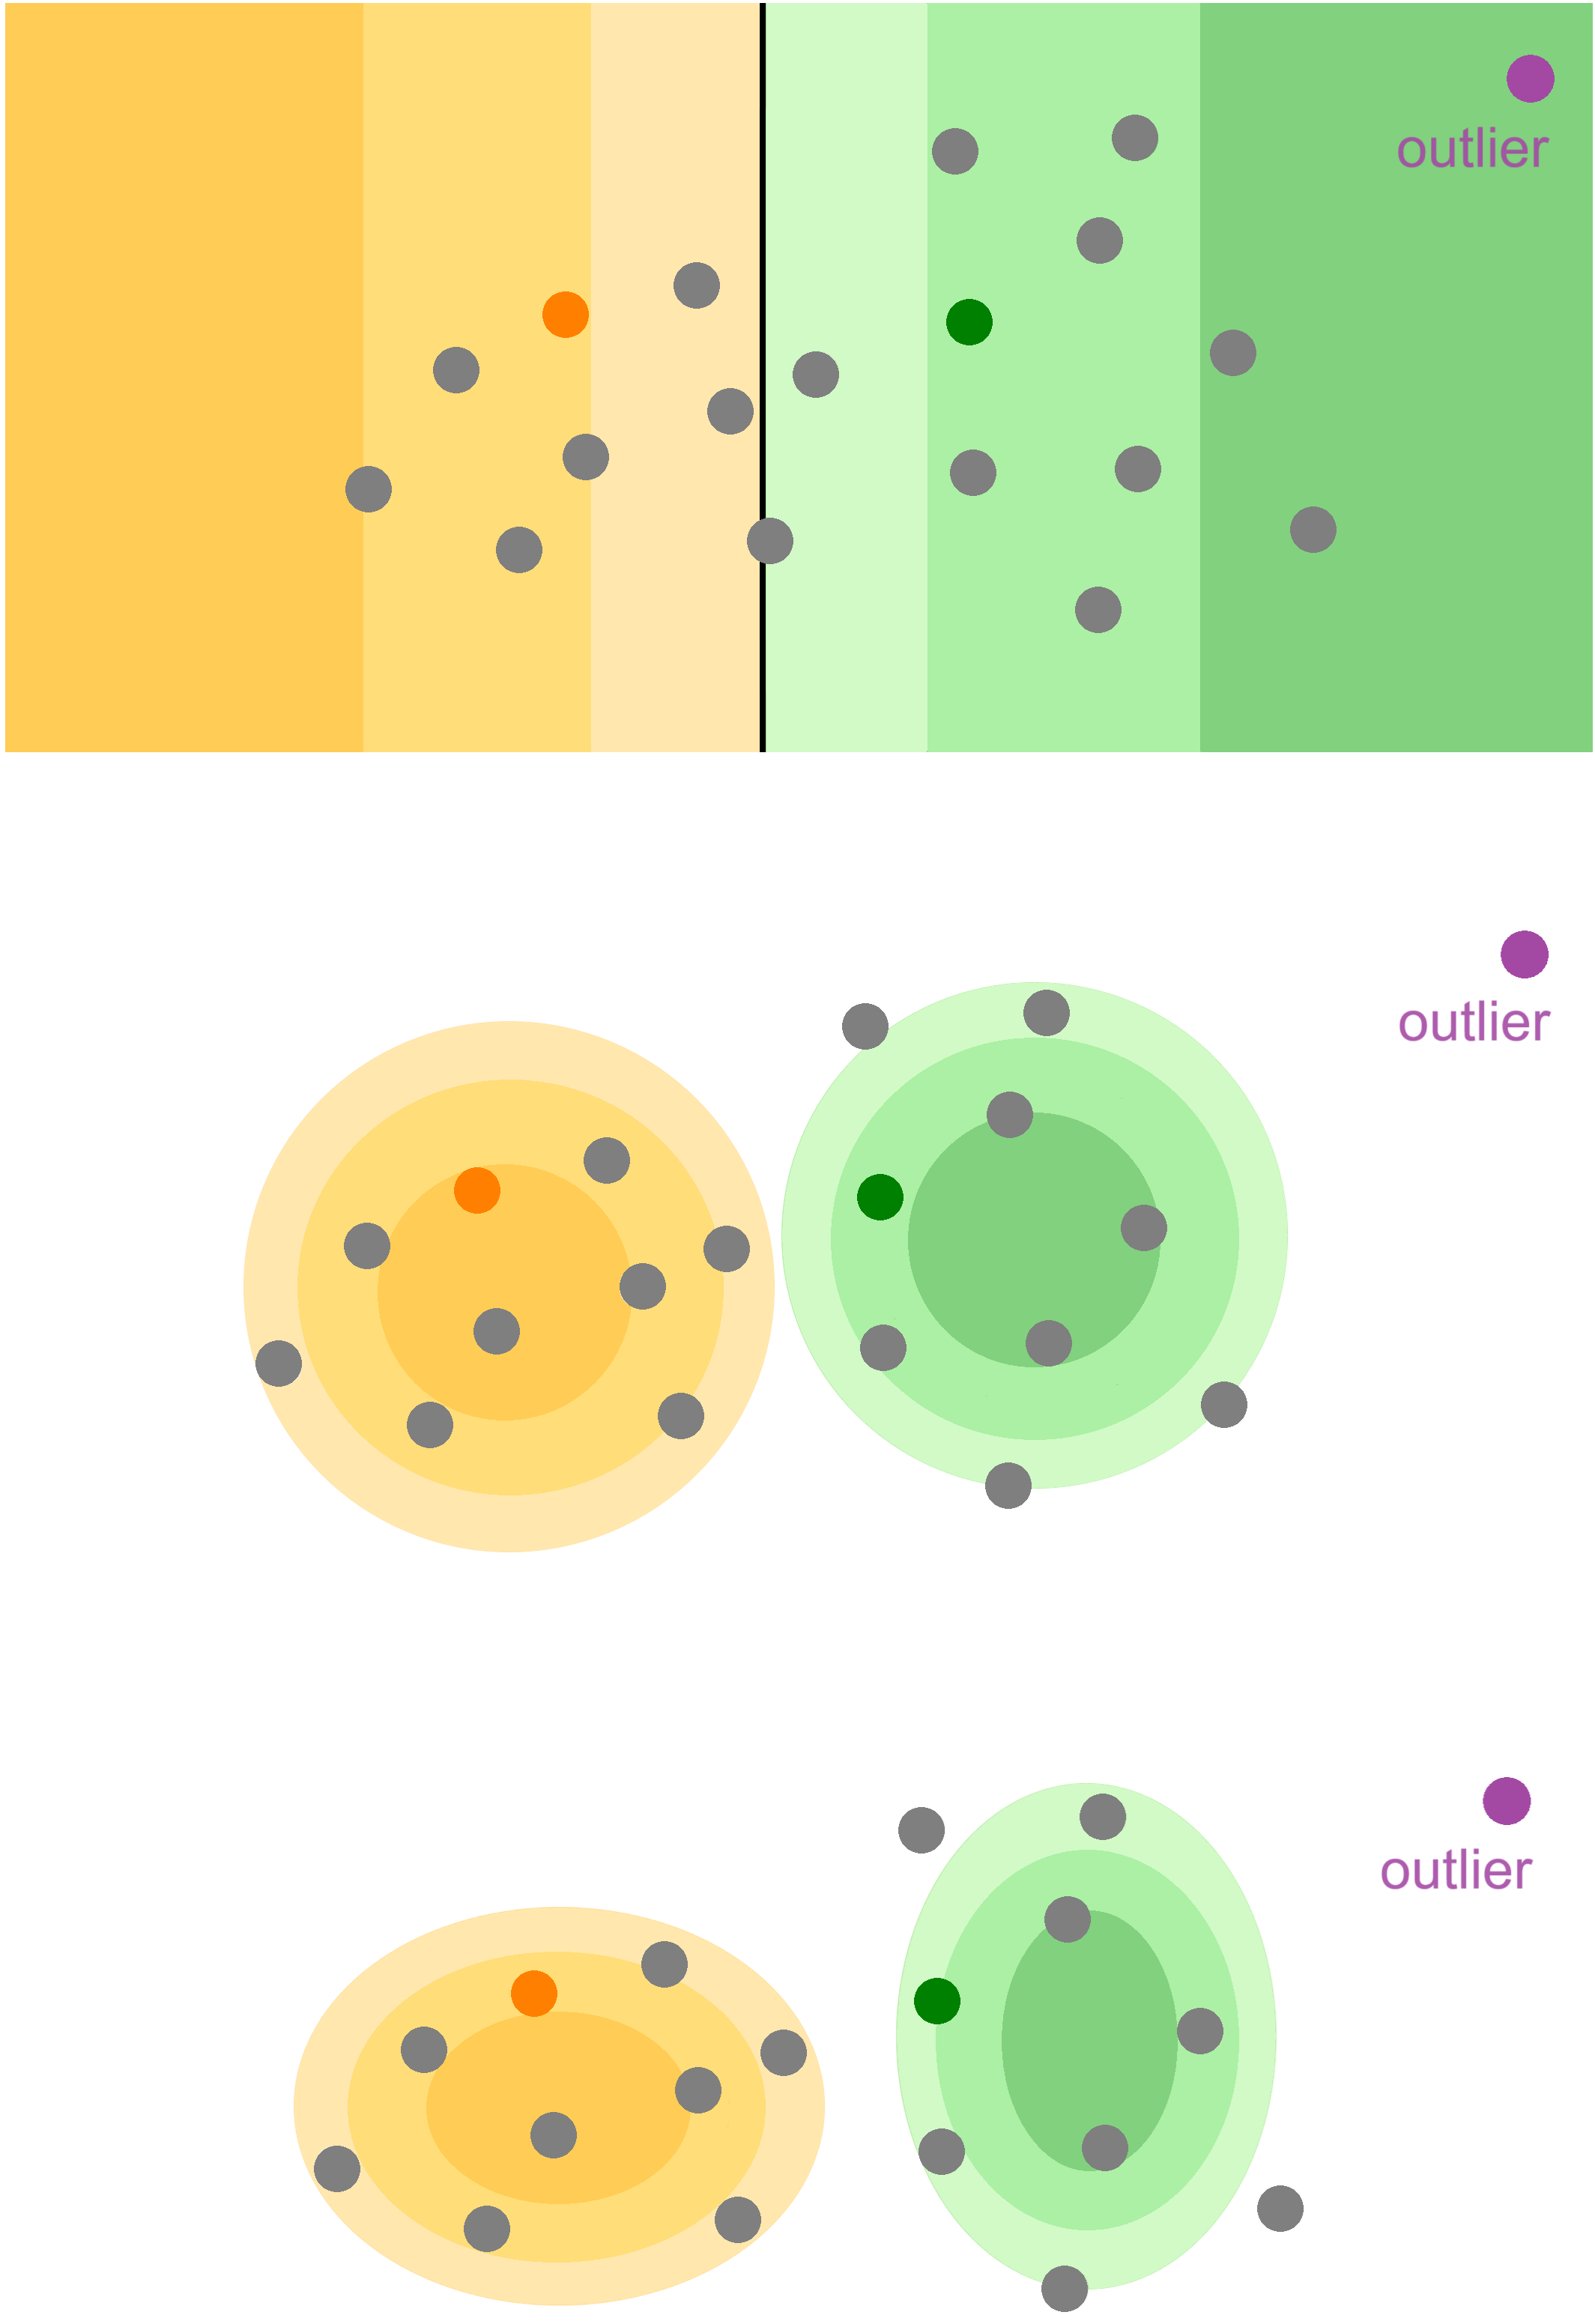
\includegraphics[width=0.75\linewidth]{figures/illustration.png}
	\caption{Schematic of the outlier problem, and how generative modeling of the joint probability can improve the situation.  Prediction with (top) fully-superivsed softmax (middle) semi-supervised KMeans and (bottom) semi-supervised AAGMM.} 
	\label{fig:schema}
\end{figure}

\begin{figure*}[ht]
	\centering
	\begin{subfigure}[t]{.24\textwidth}
		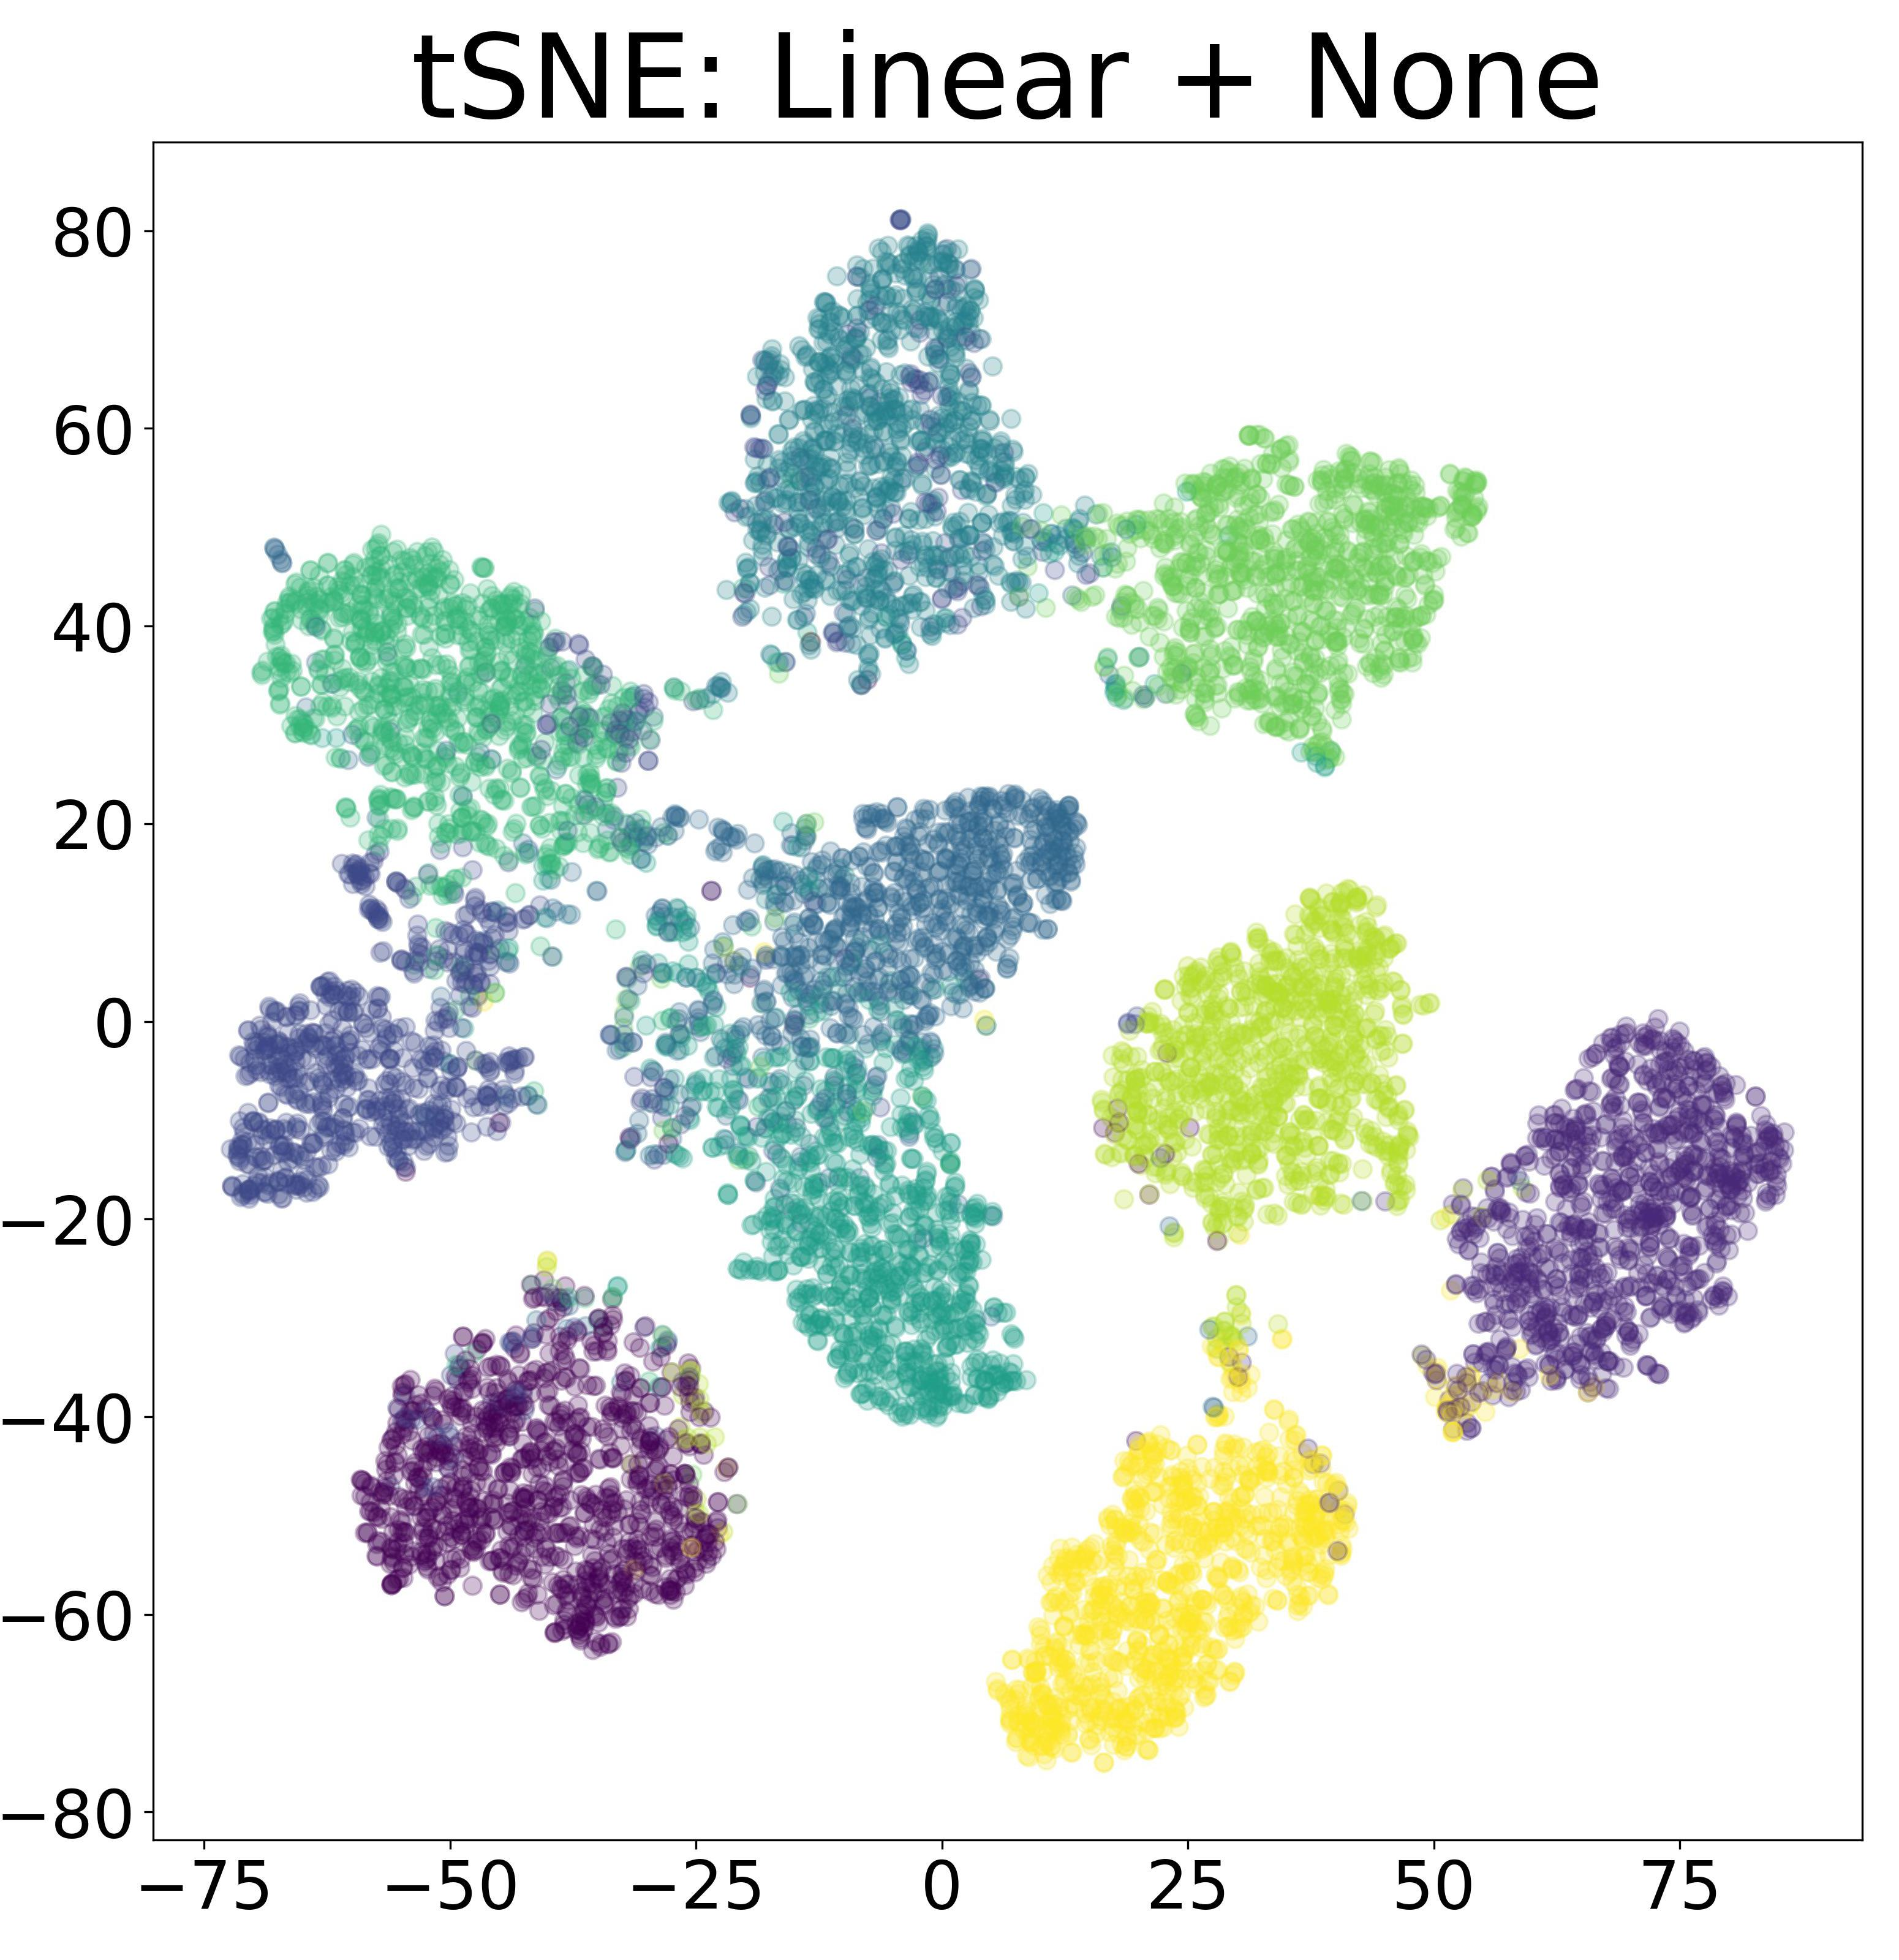
\includegraphics[width=\textwidth]{figures/id-00000001-tsne.jpg}
		\subcaption{}
	\end{subfigure}
	\begin{subfigure}[t]{.24\textwidth}
		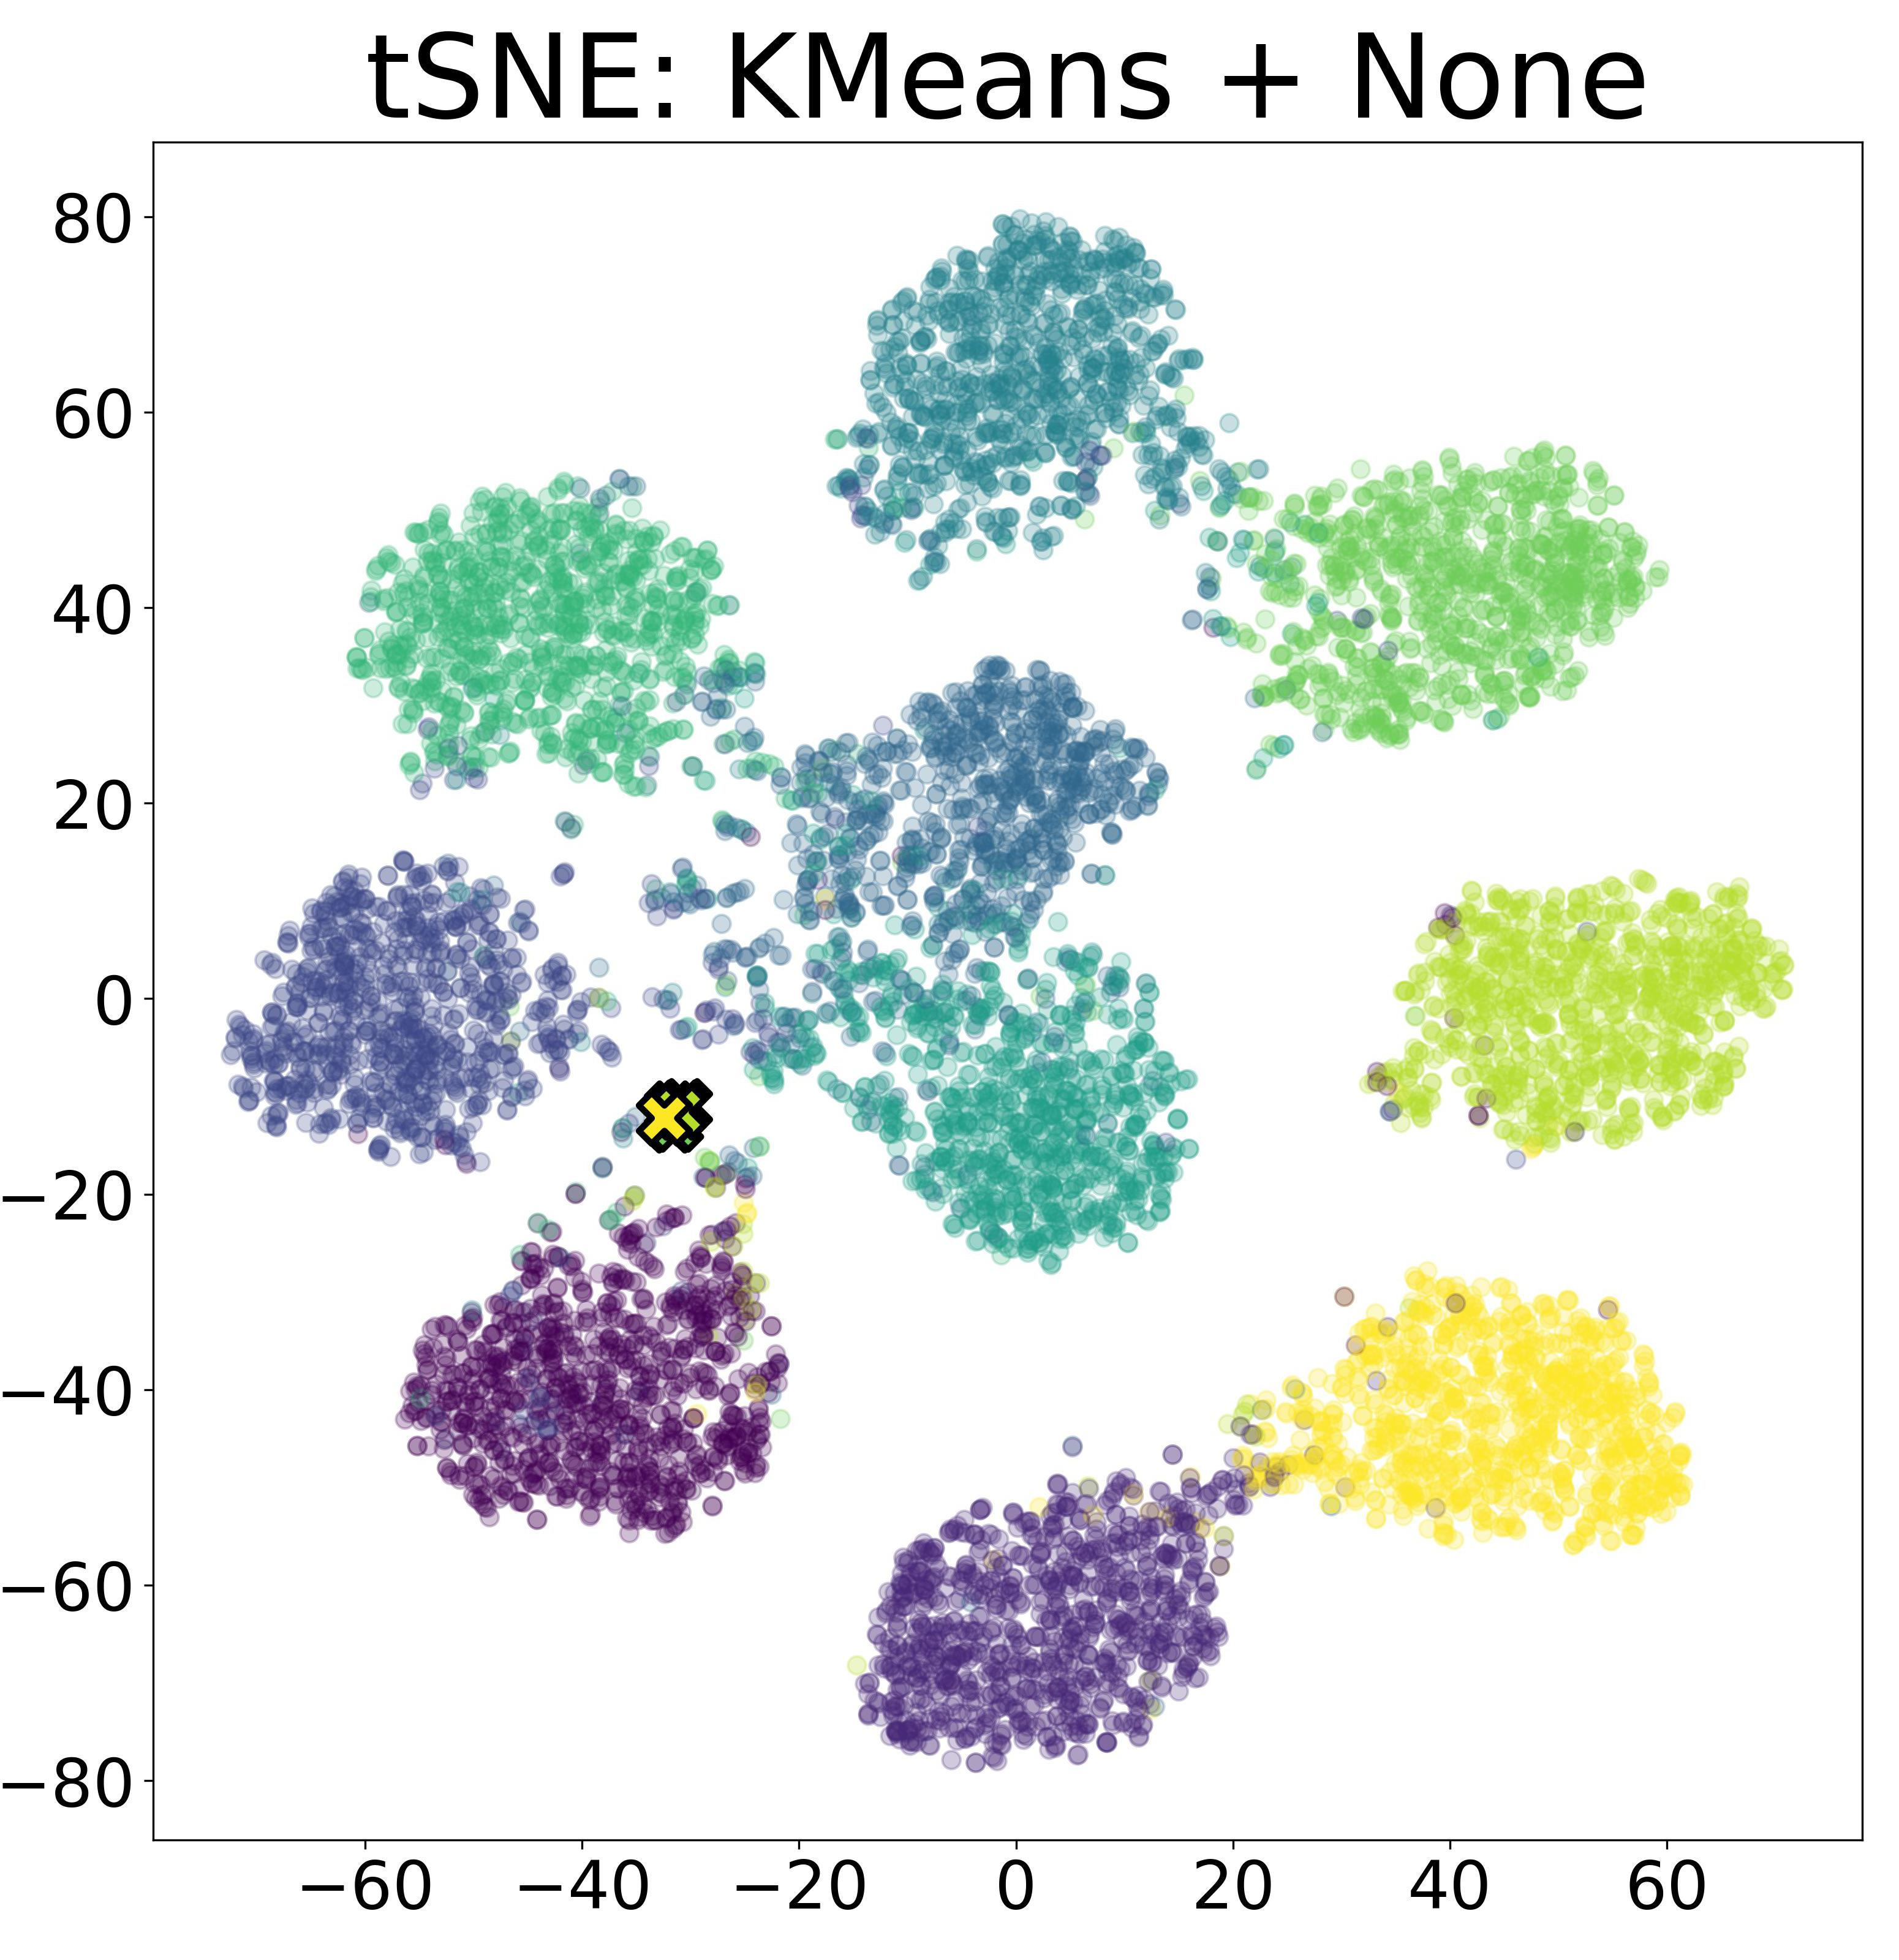
\includegraphics[width=\textwidth]{figures/id-00000013-tsne.jpg}
		\subcaption{}
	\end{subfigure}
	\begin{subfigure}[t]{.24\textwidth}
		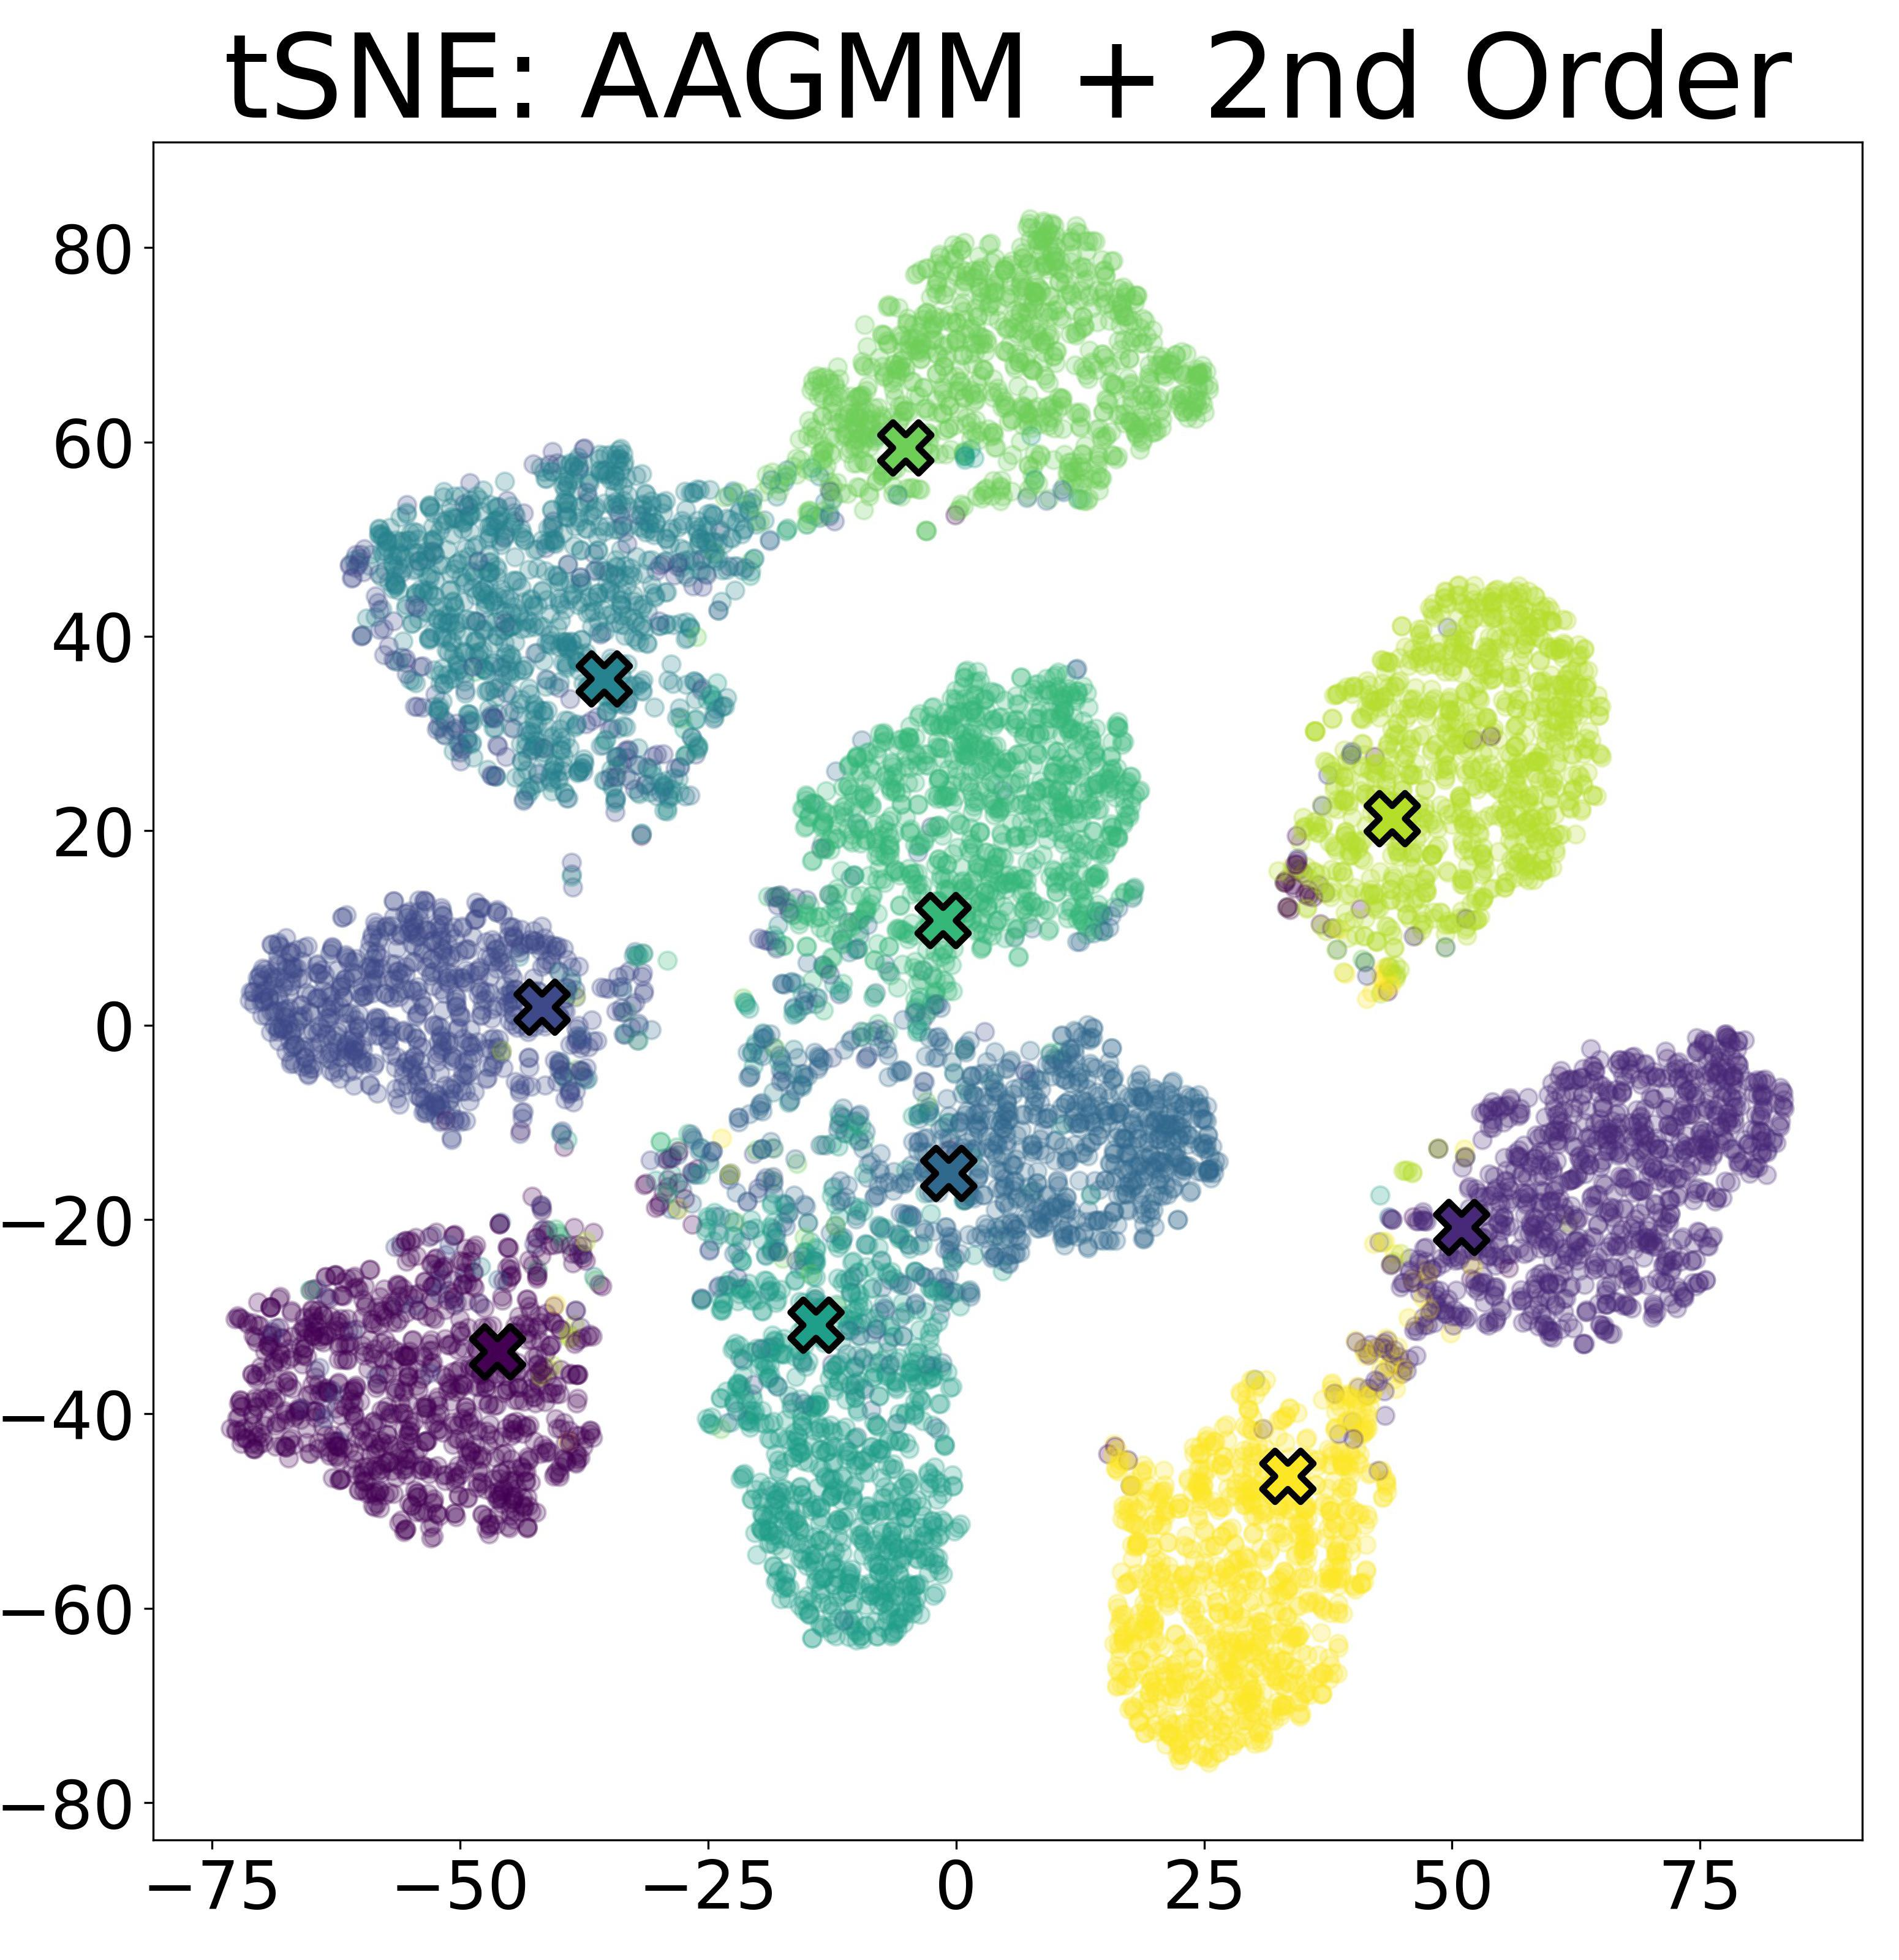
\includegraphics[width=\textwidth]{figures/id-00000054-tsne.jpg}
		\subcaption{}
	\end{subfigure}
	\begin{subfigure}[t]{.24\textwidth}
		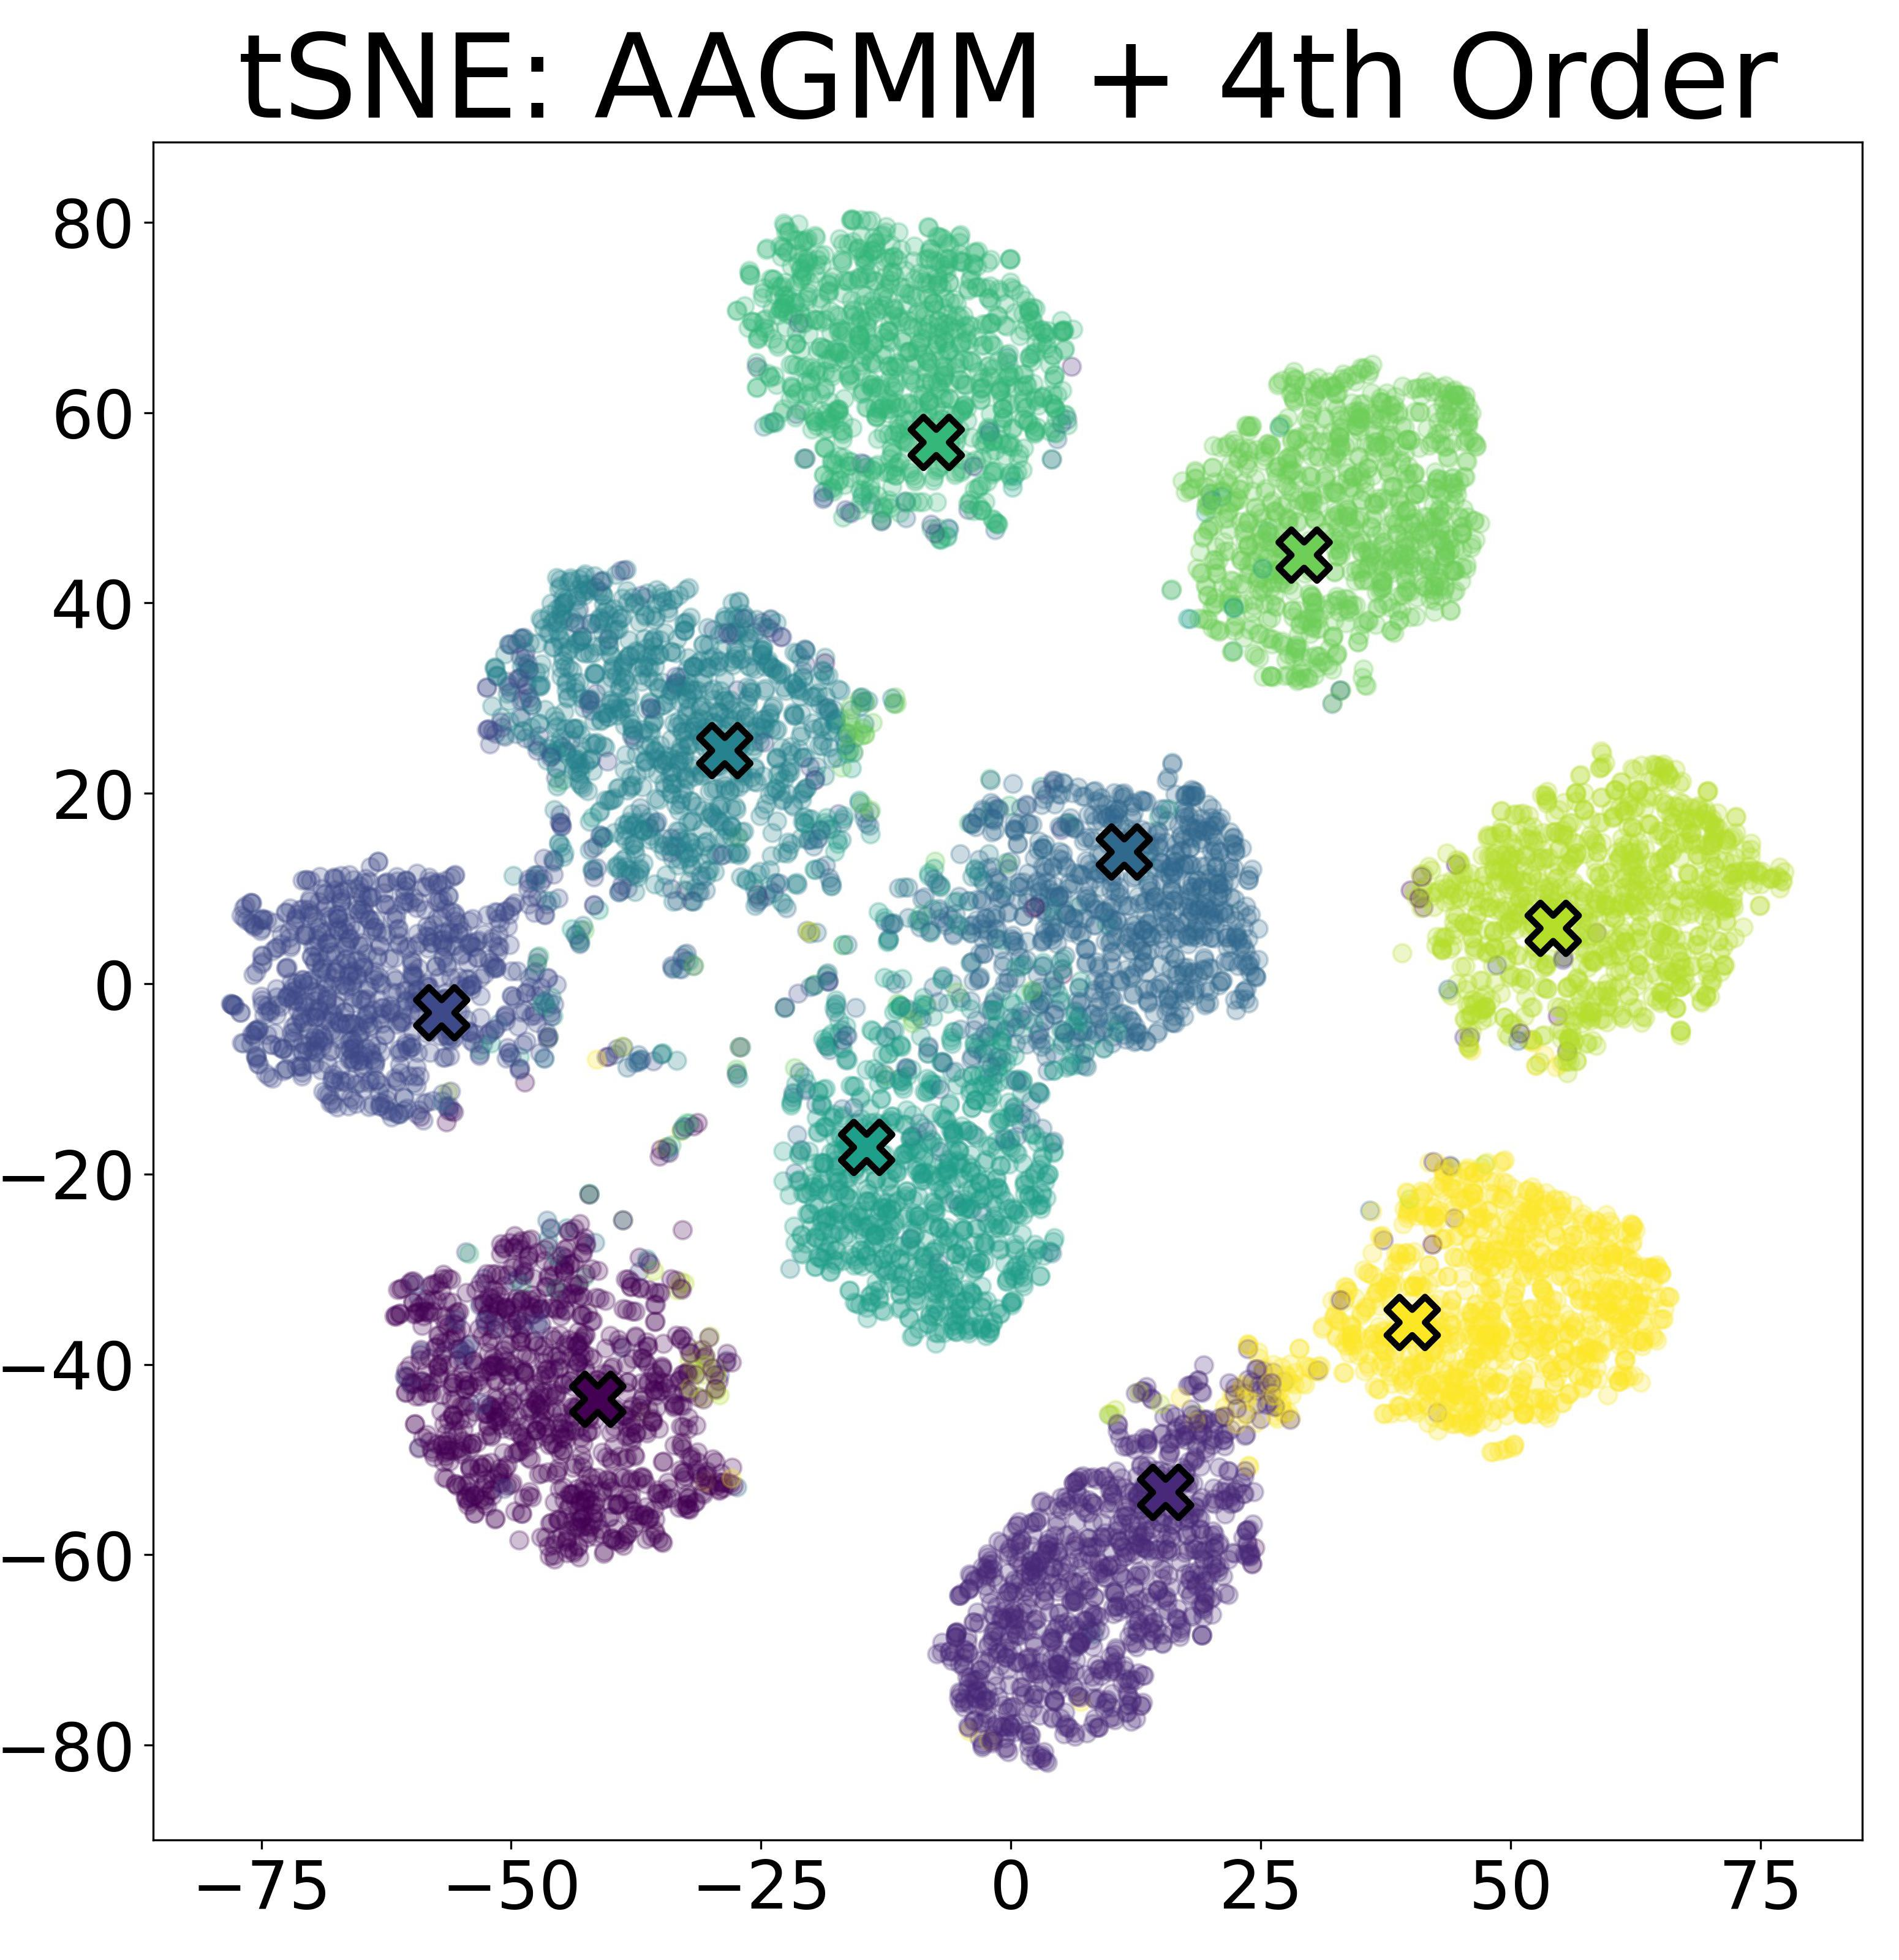
\includegraphics[width=\textwidth]{figures/id-00000021-tsne.jpg}
		\subcaption{}
	\end{subfigure}
	%	\subfloat{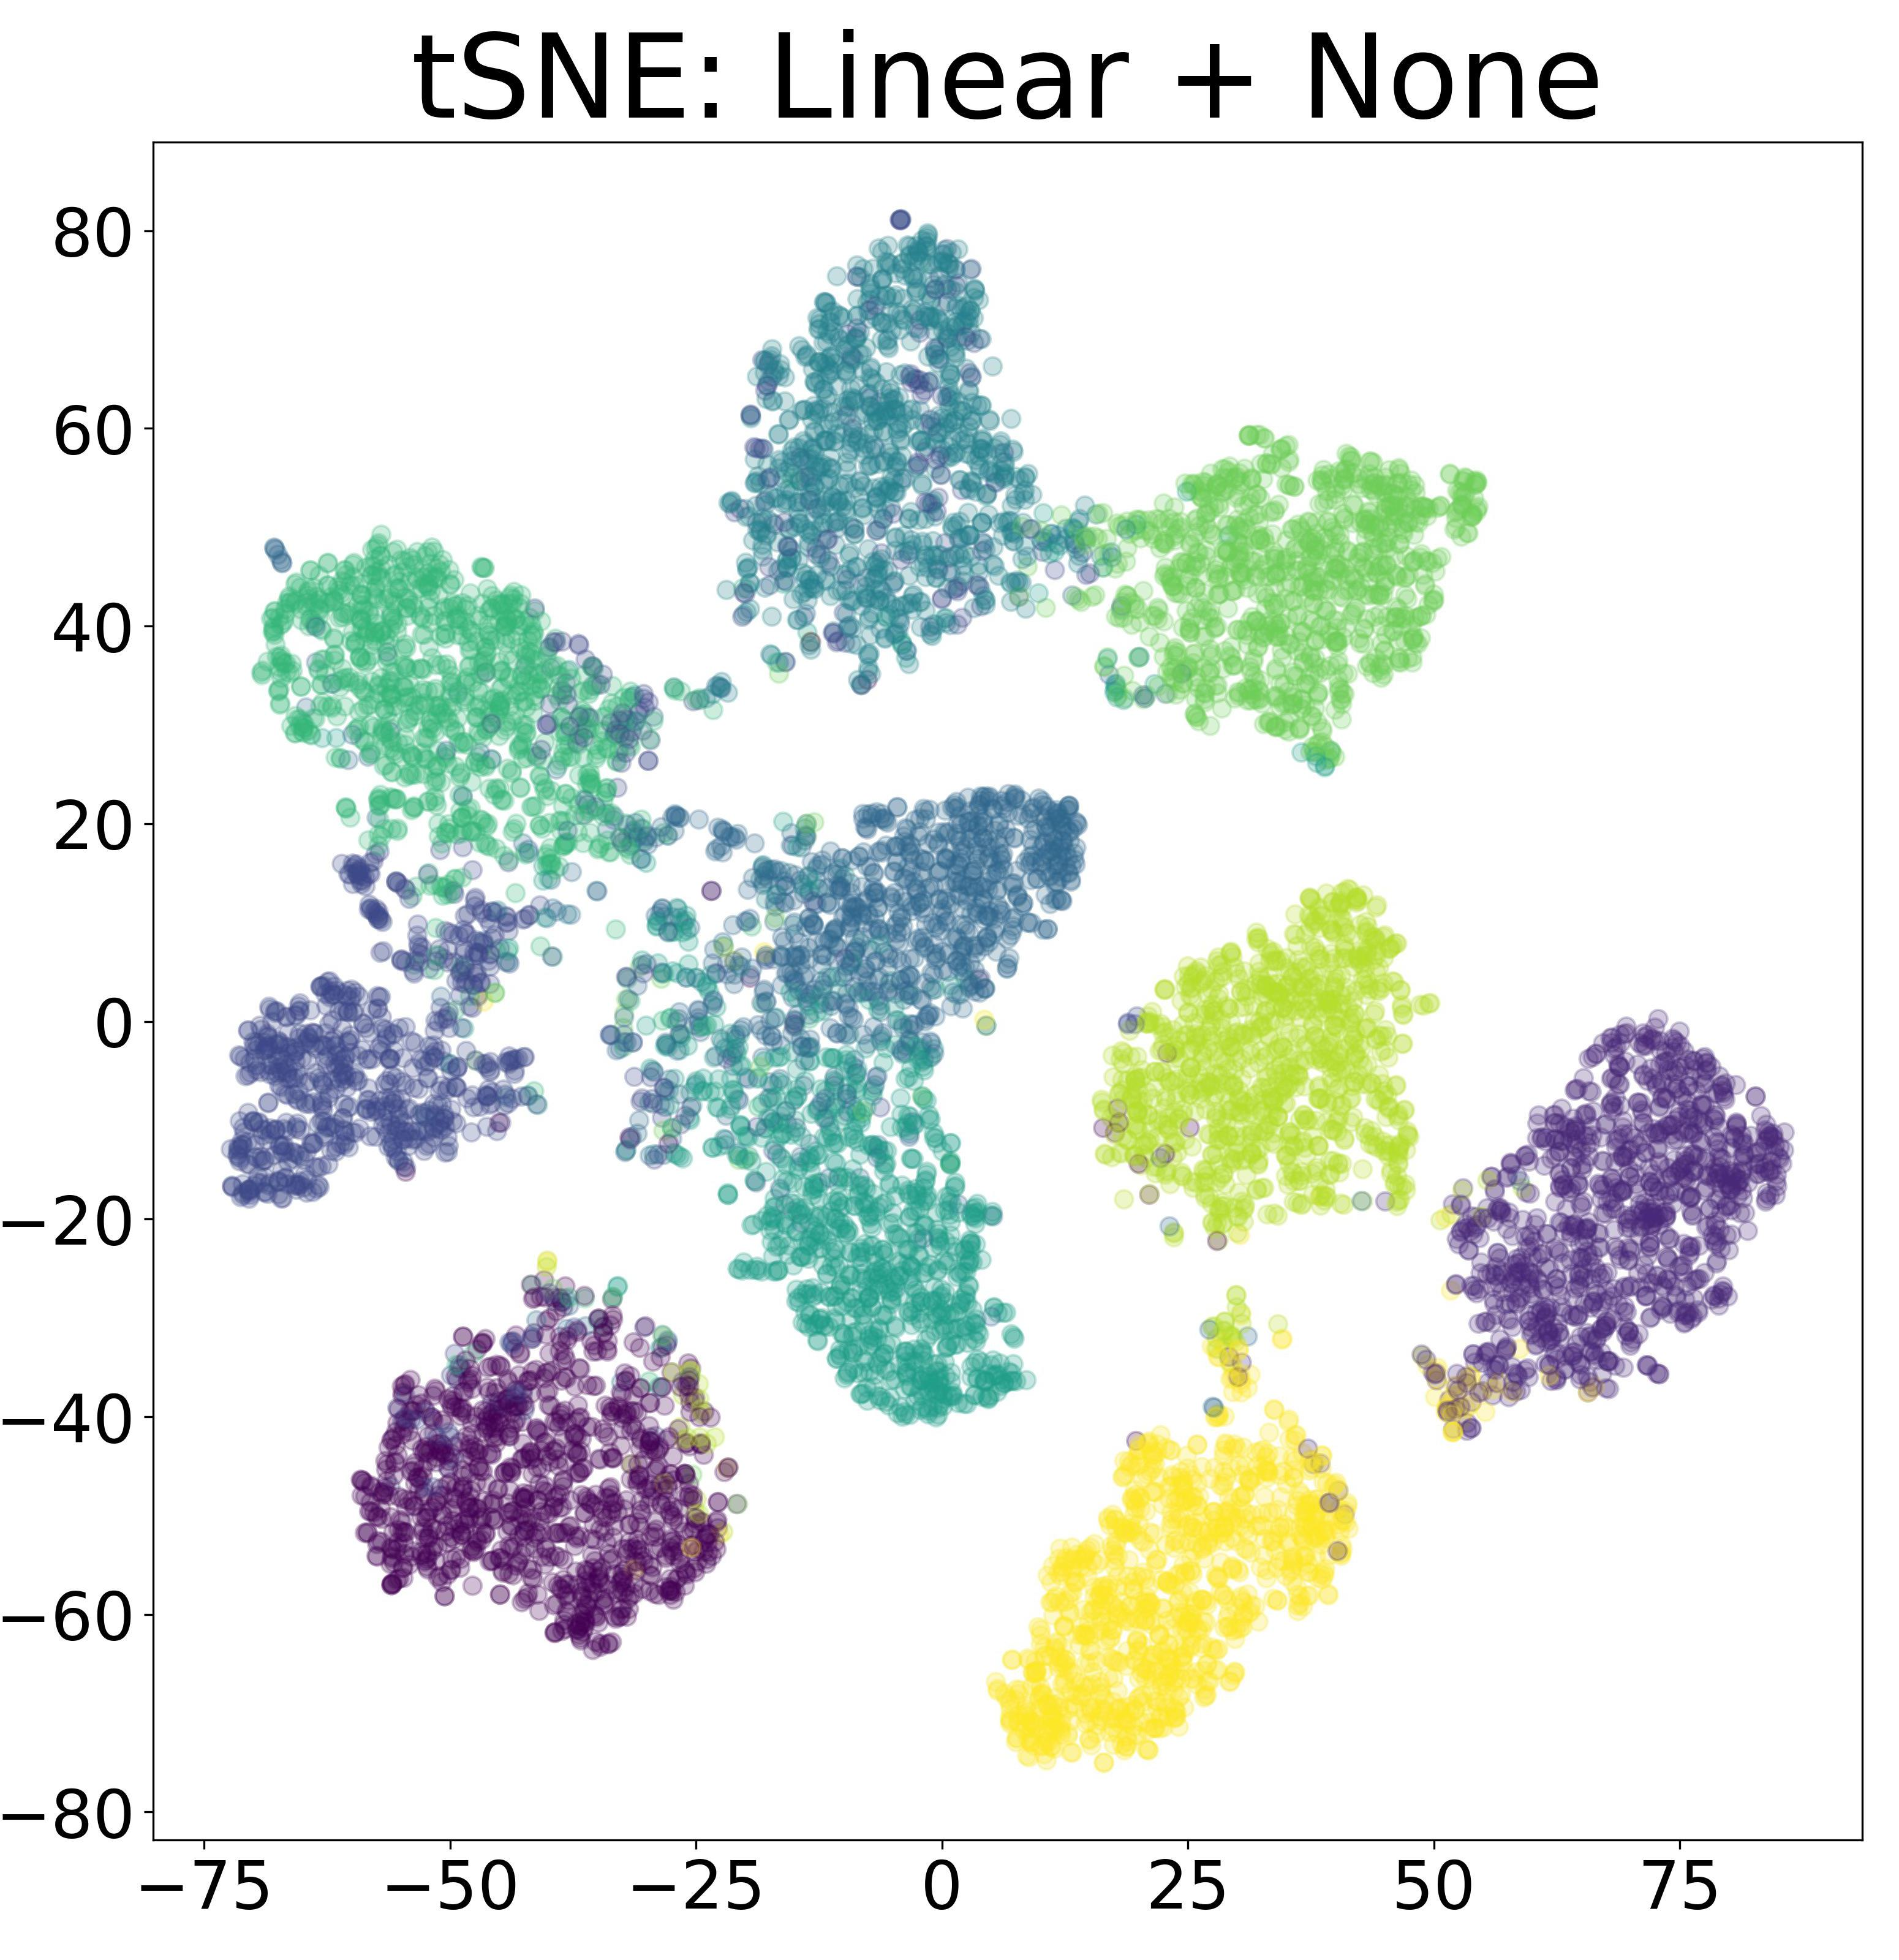
\includegraphics[width=.25\textwidth]{figures/id-00000001-tsne.jpg}}
	%	\subfloat{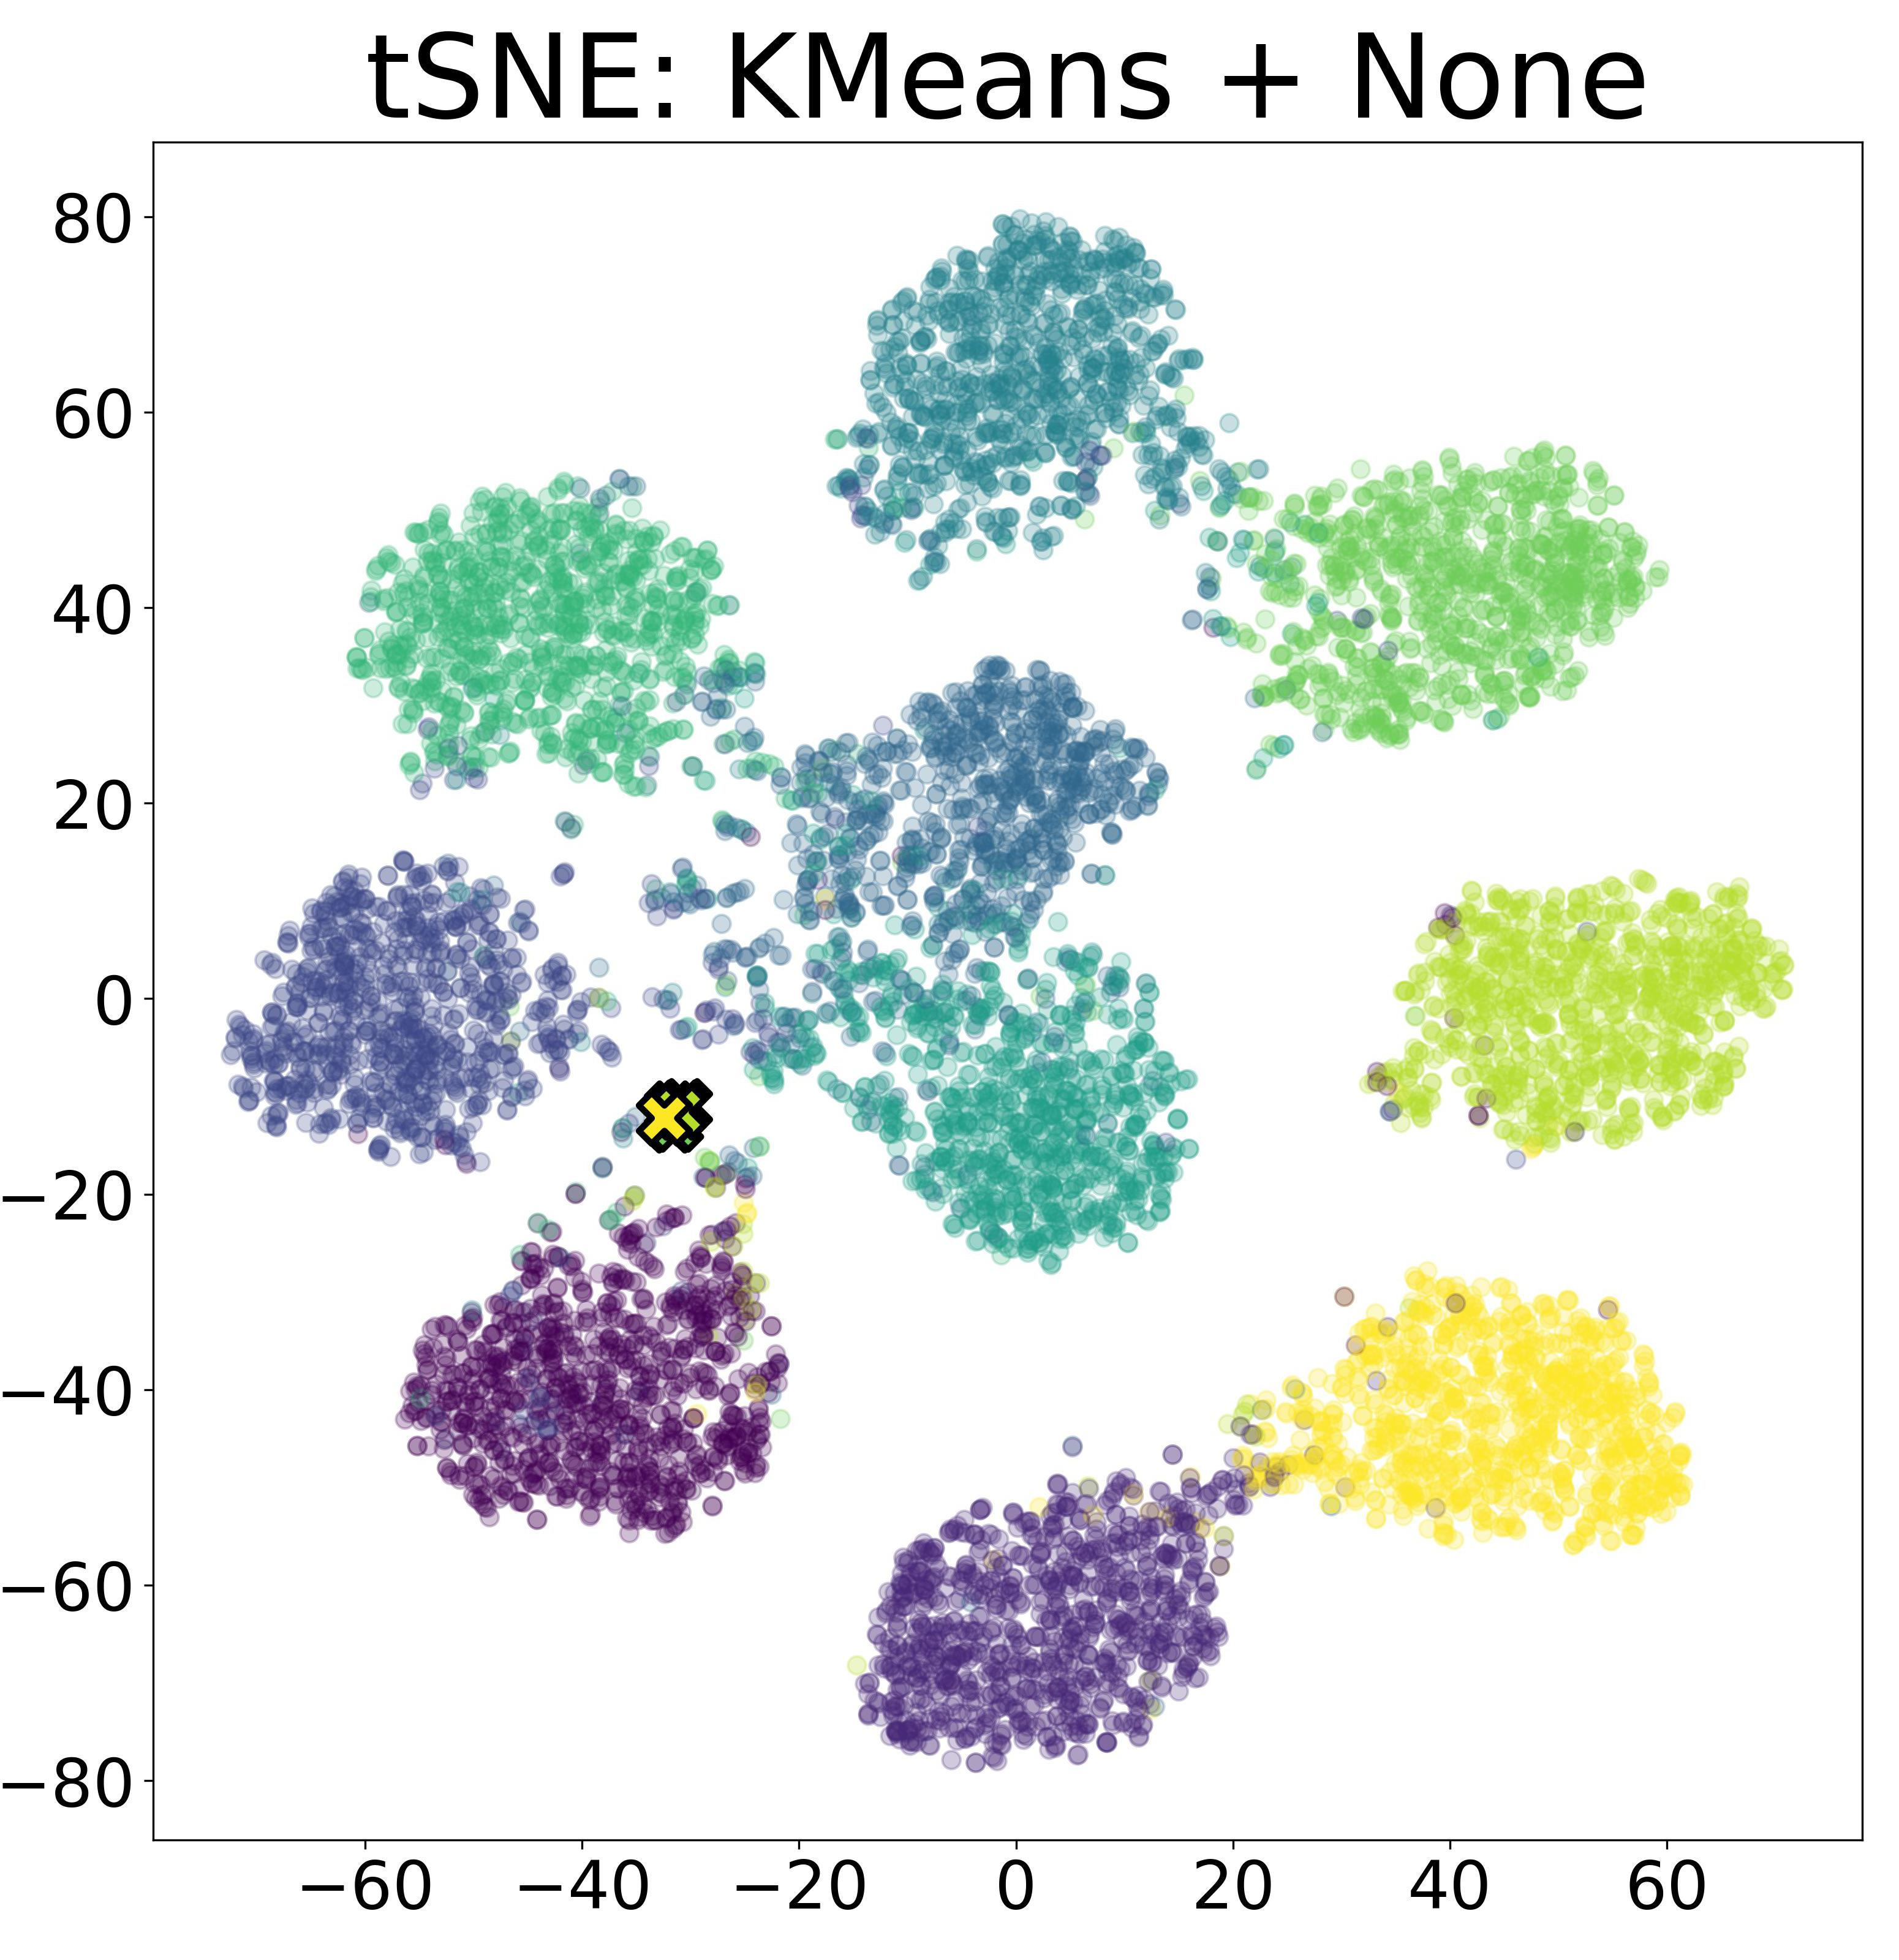
\includegraphics[width=.25\textwidth]{figures/id-00000013-tsne.jpg}}
	%	\subfloat{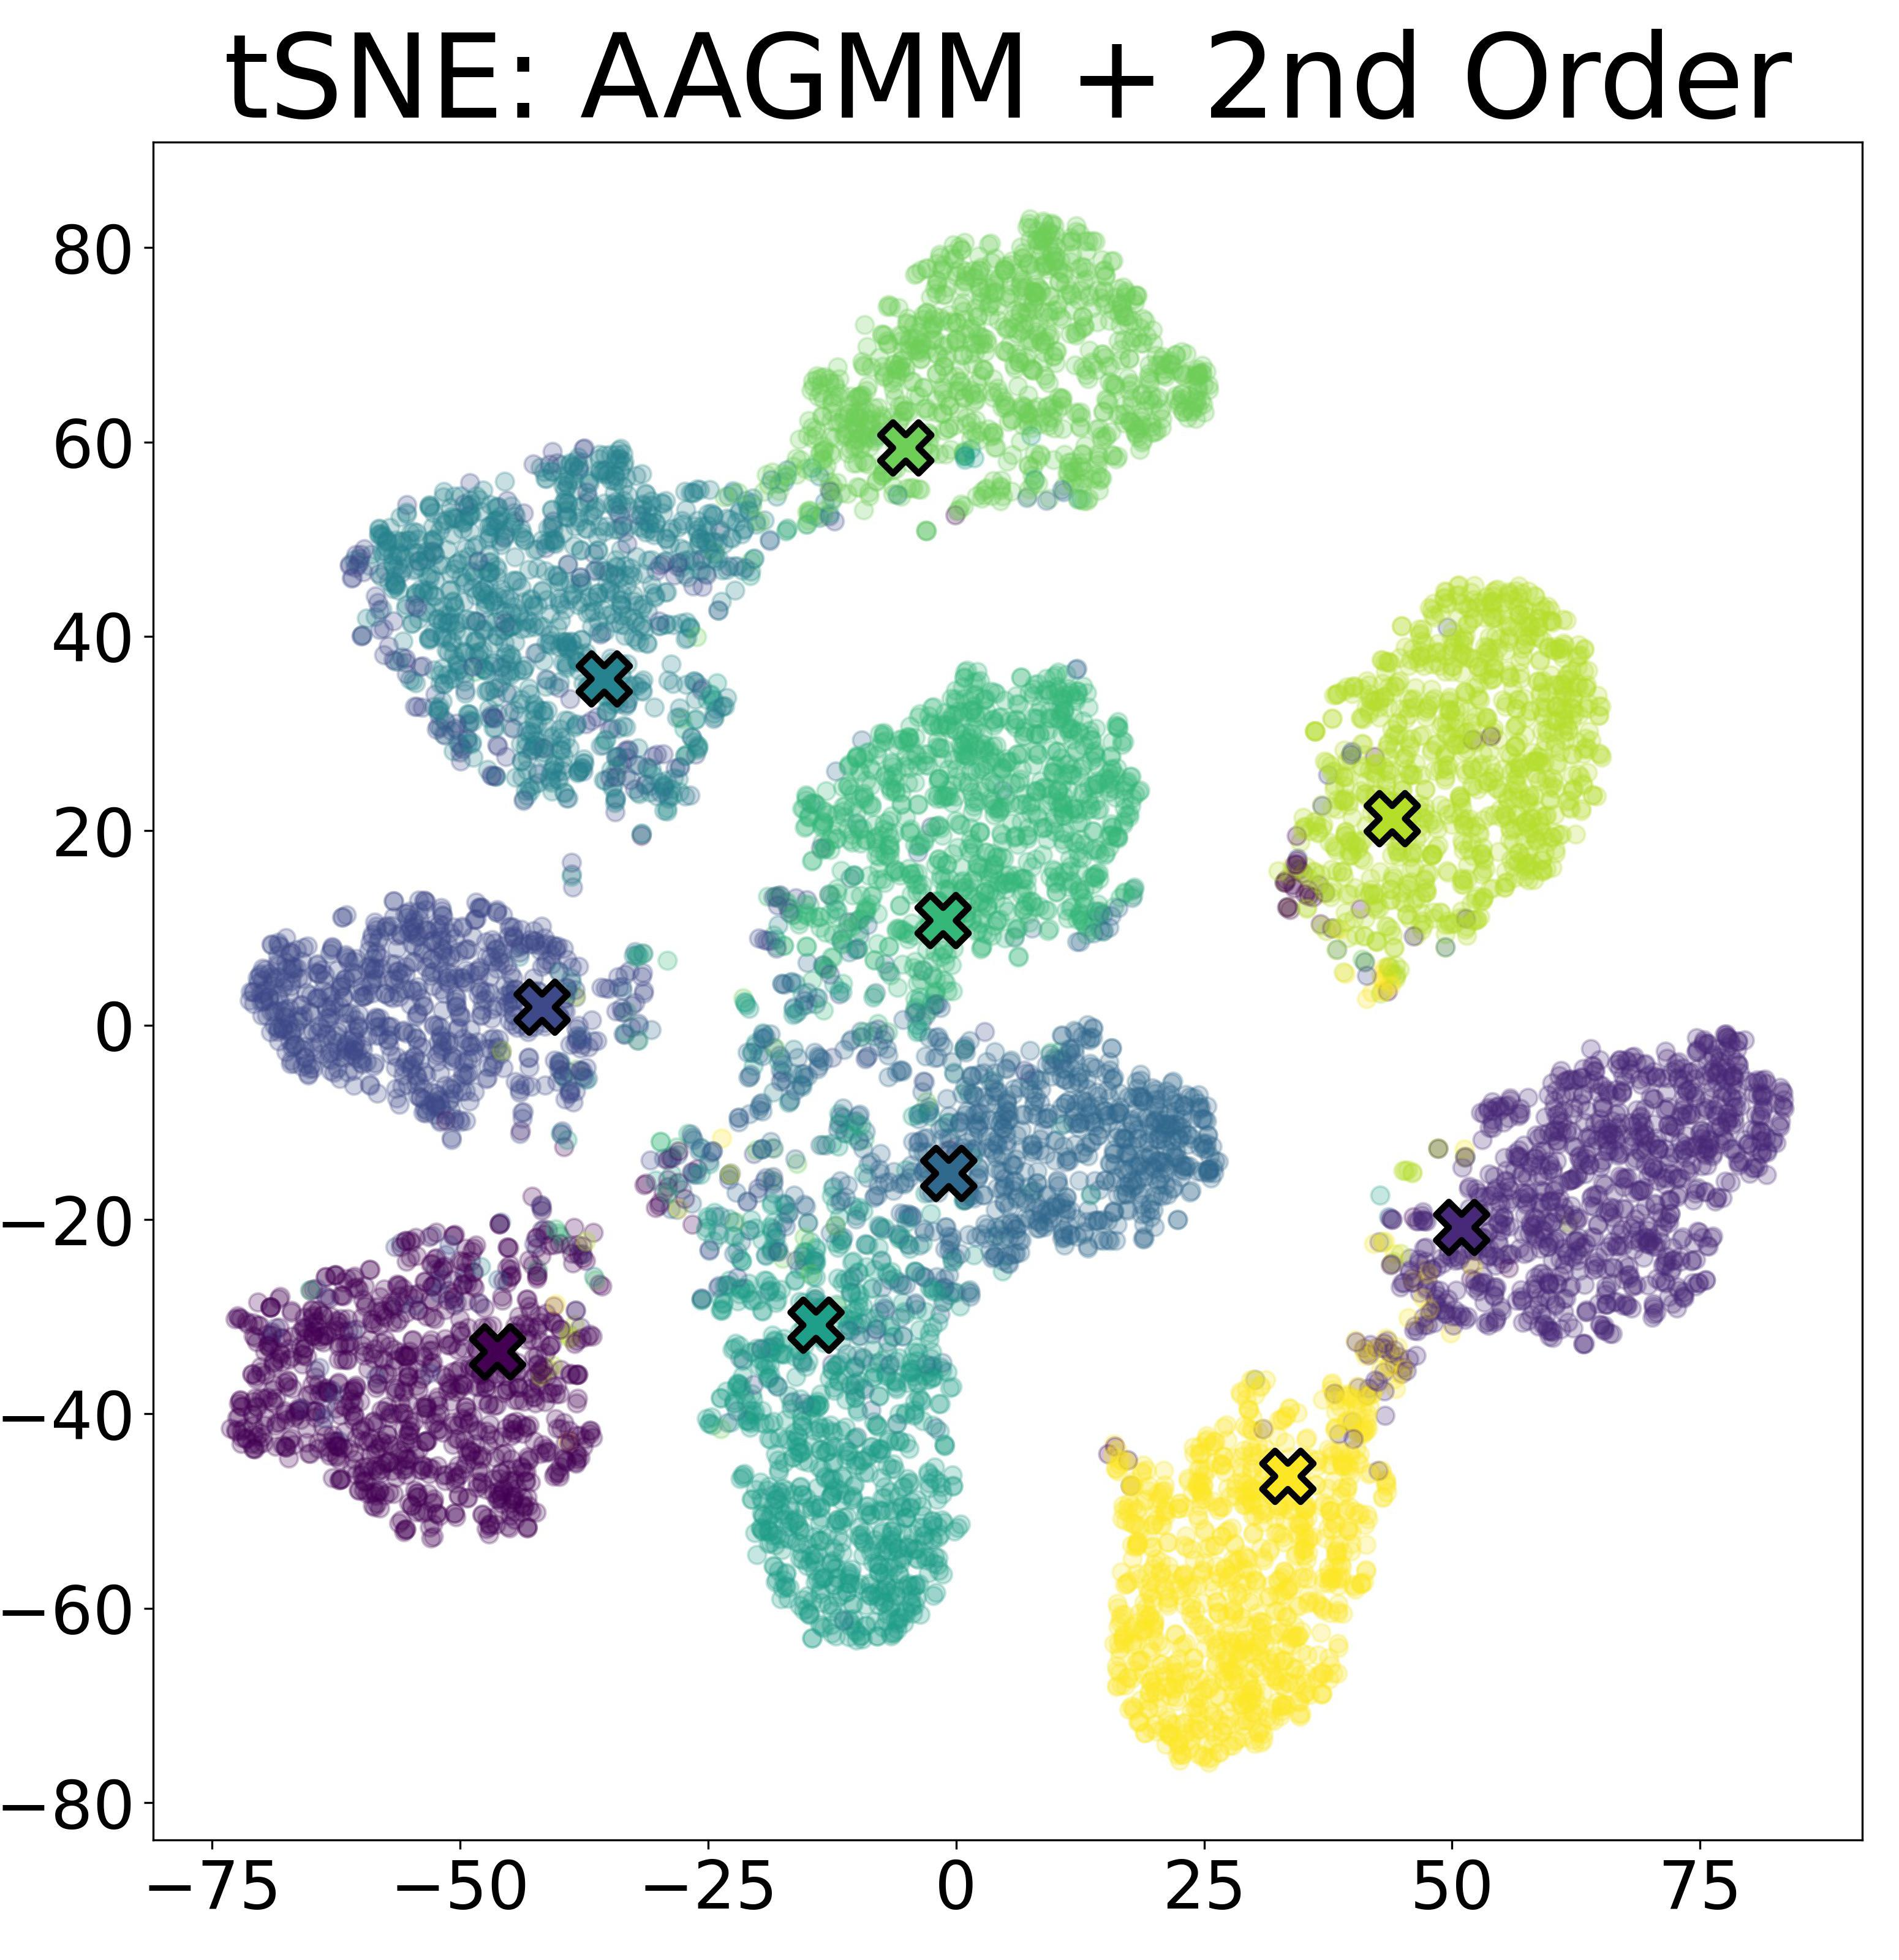
\includegraphics[width=.25\textwidth]{figures/id-00000054-tsne.jpg}}
	%	\subfloat{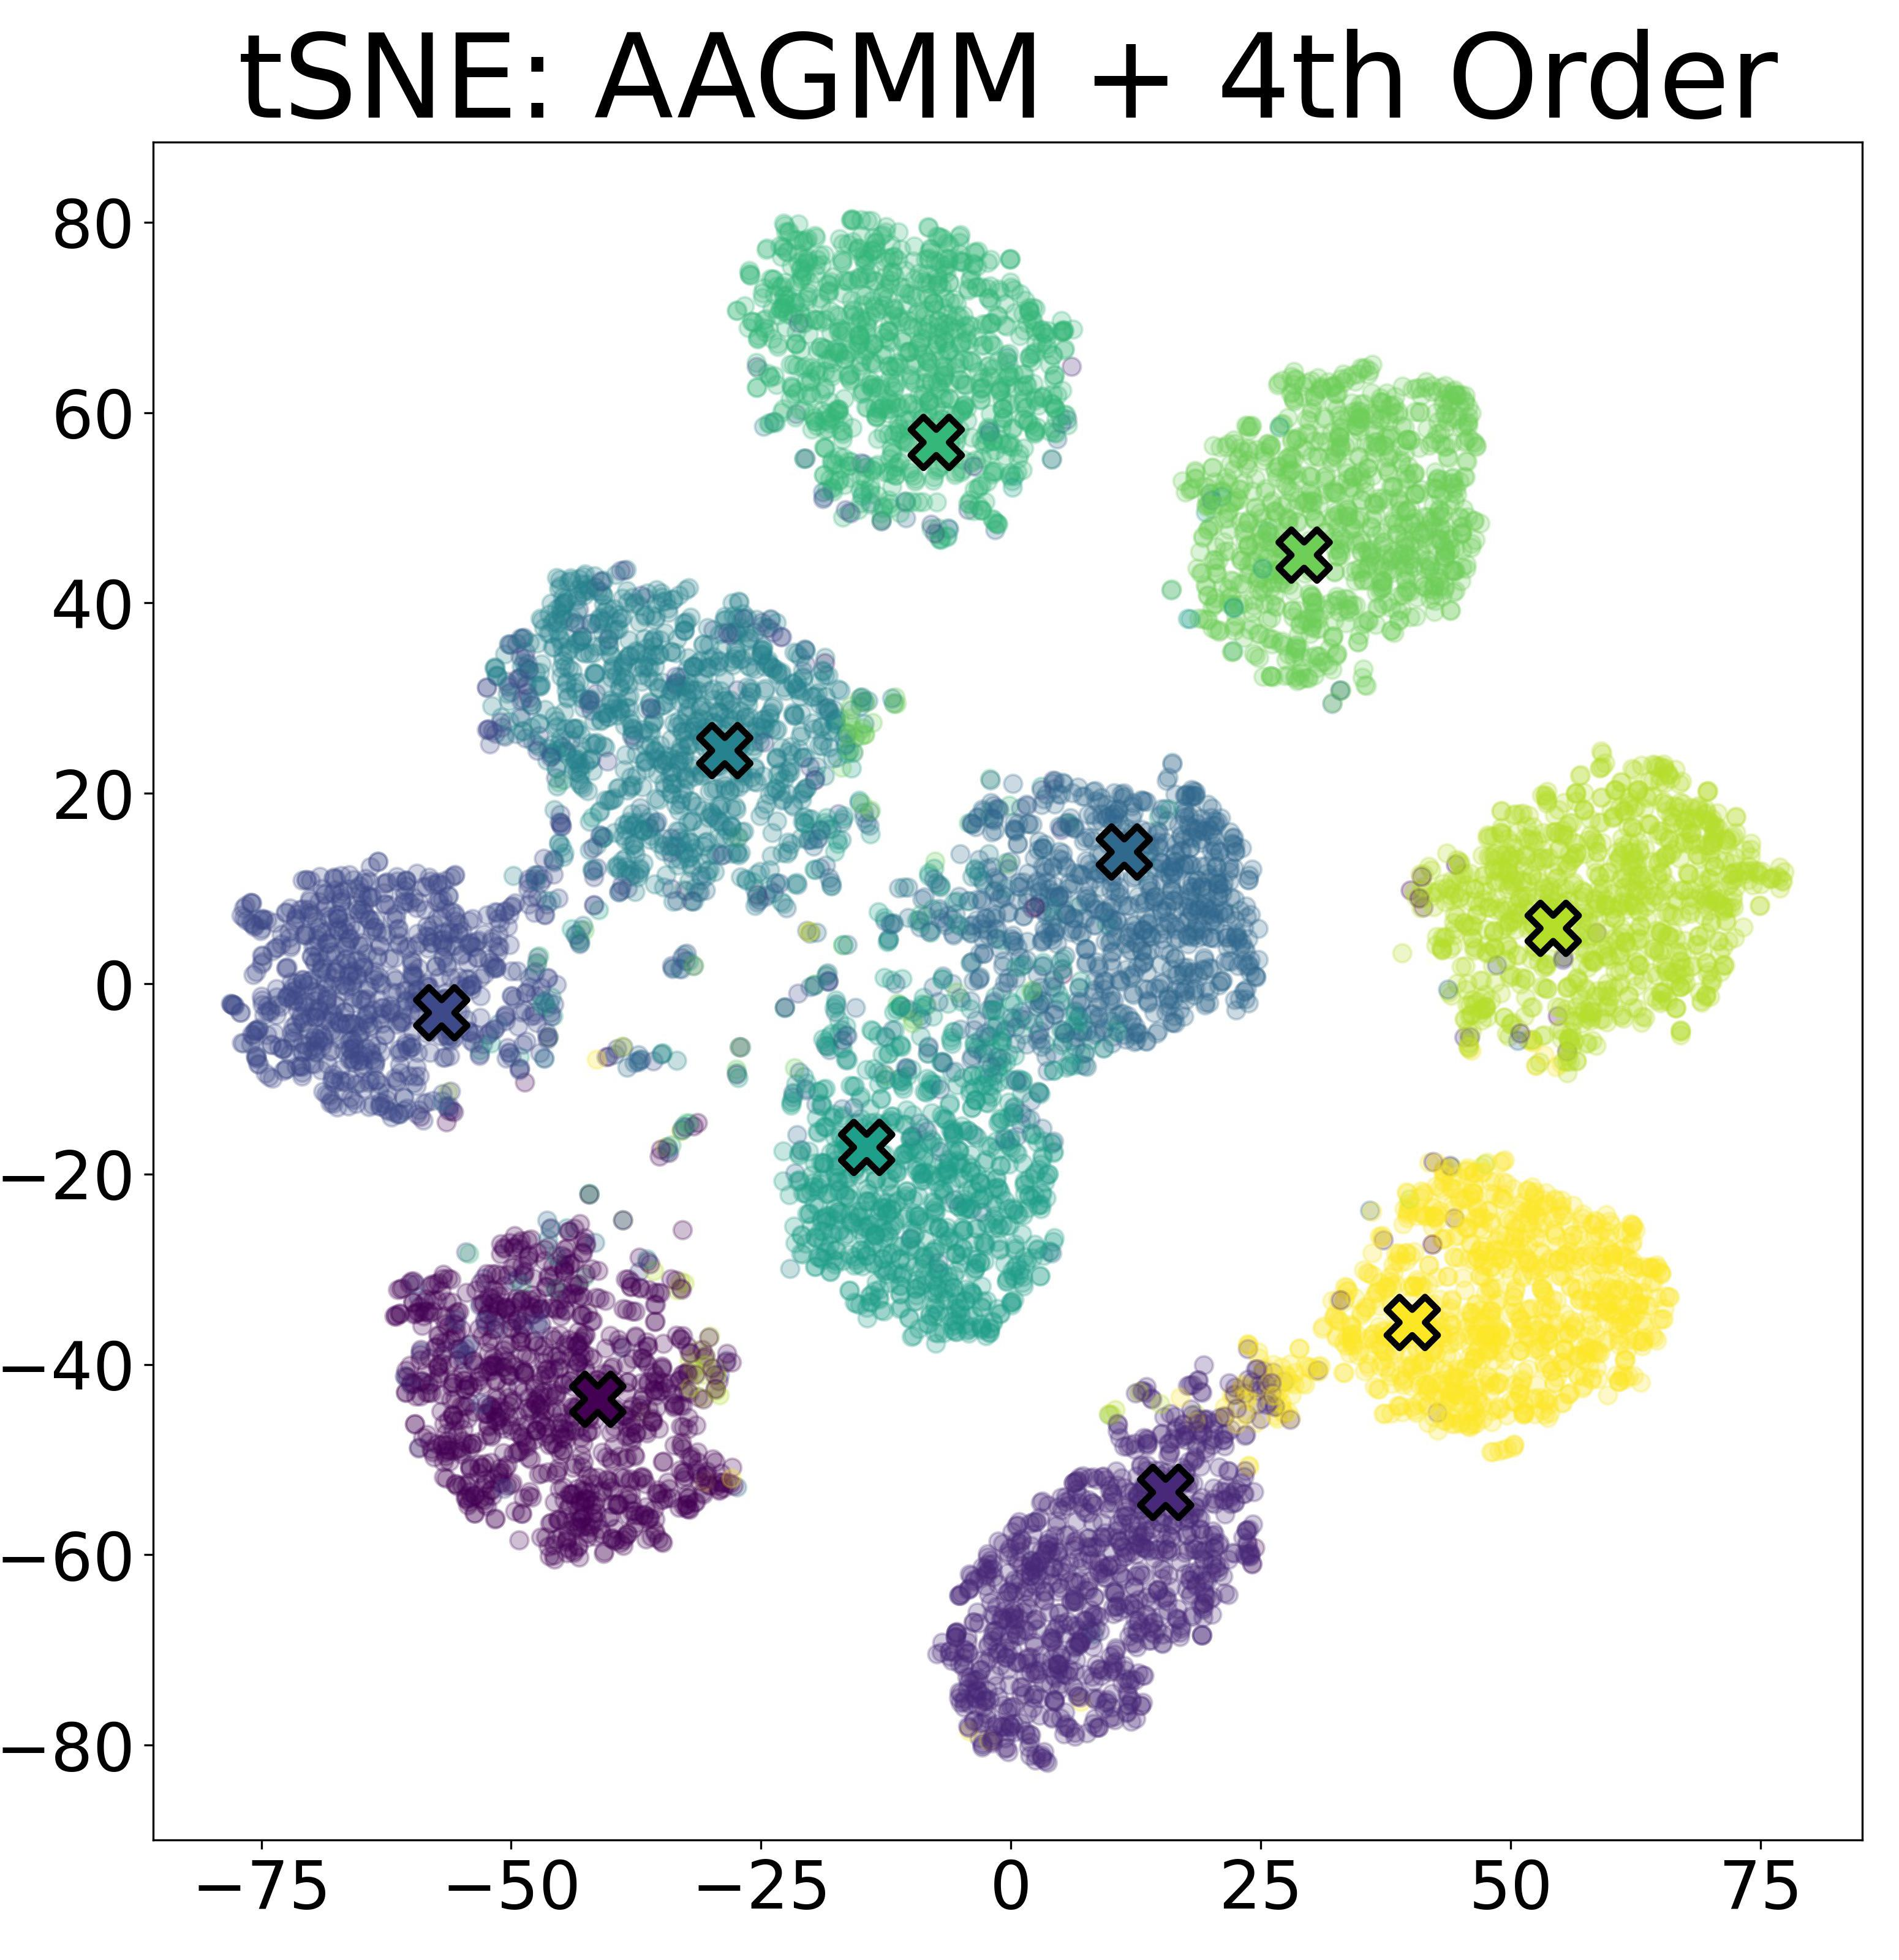
\includegraphics[width=.25\textwidth]{figures/id-00000021-tsne.jpg}}
	\caption{t-SNE\cite{tsne} plot of the latent embedding space for various final layers with different MoM embedding constraints.} 
	\label{fig:cifar10tsne}
\end{figure*}

The majority of deep classifiers rely on a softmax final activation layer which predicts the conditional probability $p(y|x)$.
When that layer receives input $x$, the model predicts a soft psuedo-distribution of labels $y$ which argmax can convert into a hard label.
If $x$ is far from the decision boundary, then by definition, softmax assigns a prediction $y$ with high confidence.
This works well for inlier samples, well represented by the training distribution.
However, when presented with an outlier $x$, it is likely $x$ will be far from the decision boundary (Figure \ref{fig:schema}, top).
Therefore softmax perceptrons, by definition, over-confidently hallucinate when given unexpected inputs \cite{wei2022mitigating}. 
Most deep classifiers use softmax without a safety net and thereby over-confidently predict $y$.
Ideally, when input $x$ is far from the decision boundary and training exemplars, the model should not be confident about the output class label $y$.

Replacing softmax with a generative method that models the joint probability $p(y,x)$ can improve the capability of deep classifiers. 
Models using a final layer capable of learning the joint probability $p(y,x)$ can infer the conditional $p(y|x)$.
More importantly, such a layer can also infer the prior probability $p(x)$.
Thus, if $x$ is an unexpected input, then such layer can flag the input as a low-probability outlier, rather than confidently predicting a label.

Prior work has explored generative modeling for image classification \cite{li2019disentangled,kingma2013auto,kingma2019introduction}.
Open questions remain of how to best train and utilize generative modeling within a deep learning context.
The naive approach of minimizing cross entropy between $y$ and $y\_pred$ will not work.
Figure \ref{fig:cifar10tsne} (b) shows t-SNE plots for semi-supervised CIFAR-10 \cite{cifar10} image classification which illustrate why the naive approach will not work as intended. 
The t-SNE\cite{tsne} plot of "KMeans + None" shows the latent space of a $93\%$ accurate CIFAR-10 classification model. 
However, the explicitly modeled cluster centers (shown as X's) do not align with the underlying data.
While that model has acceptable predictive performance, it does not accurately learn and represent the underlying training data.
To construct a robust model, one cannot simply fit a decision boundary.
The model needs to learn the full joint distribution of the latent space. 
Figure \ref{fig:cifar10tsne} (d) demonstrates that with our proposed AAGMM final layer with 4th order MoM embedding constraints, the exact same model can achieve comparable (if not better) accuracy, but with the added benefit of modeling the underlying data clusters in the latent space.


We apply this work to the domain of Semi-Supervised Learning (SSL), because over-confident label predictions can cause confounding issues with pseudo-labeling methods \cite{arazo2020pseudo}.
%This is equivalent to improving the accuracy of class inlier determination.
%As such SSL is an excellent application to test generative final activation layers which model the joint probability $p(y,x)$, thereby enabling estimation of both the conditional $p(y|x)$ and prior $p(x)$ probabilities. 
%as pseudo-labeling methods are sensitive to outliers.
SSL leverages an abundance of unlabeled data to improve deep learning based model performance under limited training data regimes \cite{zhu2022introduction,li2019safe,hady2013semi}.
%Image classification has become a playground for exploring novel SSL ideas, of which there are several flavors.
Contrastive learning methods leverage the intuition that similar instances should be close in the representation space, while different instances are farther apart \cite{yang2022class,li2021comatch}.
Consistency regularization borrows the intuition that modified views of the same instance should have similar representations and predictions \cite{sohn2020fixmatch,lee2022contrastive,zhang2021flexmatch,kim2022conmatch}.
Pseudo-labeling methods like FixMatch \cite{sohn2020fixmatch} leverage the ideas of consistency regularization.
This work contributes:

\begin{enumerate}
	\item A novel Method of Moments (MoM) based embedding constraint that enables the model to not only learn the decision boundary but also the latent joint distribution. 
	Moreover, this constraint ensures that each latent cluster exhibits a well-behaved Gaussian shape.
	\item A replacement of the final linear+softmax final activation layer of the neural network with either an axis-aligned differentiable Gaussian Mixture Model (AAGMM) or an equal variance version named KMeans trained via back propagation, both of which have explicit modeling of class cluster centroids. 
	%\item A demonstration of the latent embedding space response to various constraints on how it should be structured by adding penalties if the per-class clustering does not conform to between 0 and 4 of the first Gaussian moments being identity/zero %\cite{pearson1936method}.
	\item A visualization of the latent embedding space, showing how it responds to the incorporation of generative final activation layers with and without MoM based embedding constraints.
\end{enumerate}

%This paper explores the impacts of replacing the final linear layer of a network with a generative model and embedding space constraints.
%This combination demonstrates improvements in final model accuracy when using pseudo-labeling methods where very few annotations are available.
We apply this methodology to the task of semi-supervised CIFAR-10 image classification with 40 and 250 training labels \cite{cifar10}. 
%) and CIFAR-100 (400 and 2500 label) benchmarks \cite{cifar10}. 
%Additionally, we explore the impact high level prescriptive constraints on the embedding space have on the resulting trained model. 
The embedding constraint penalties are applied to all unlabeled data and not just the valid pseudo-labels.  
As such our method fits the latent joint distribution across all of the unlabeled data points, an improvement on baseline pseudo-labeling methods (like FixMatch \cite{sohn2020fixmatch}) which only fit the conditional distribution to the high confidence pseudo-labels while removing low confidence pseudo-labels.


\section{Related Work}

% TODO compare our method to lee2022contrastive which uses explicit cluster centers, and draws both the valid and non valid PL to the cluster center, just like we do, we just don't have a contrastive element like they do

SSL has shown great progress in learning high quality models, in some cases matching fully supervised performance for a number of benchmarks \cite{zhang2021flexmatch}.
The goal of SSL is to produce a trained model of equivalent accuracy to fully supervised training, with vastly reduced data annotation requirements.
Doing so relies on accurately characterizing inlier vs outlier unlabeled samples.

\subsection{Pseudo-Labeling}
Self-training was among the initial approaches employed in the context of SSL to annotate unlabeled images. 
This technique involves the initial training of a classifier with a limited set of labeled samples and incorporates pseudo-labels into the gradient descent process, exceeding a predefined threshold \cite{yarowsky1995unsupervised, mcclosky2006reranking, olivier2006semi,zhai2019s4l,livieris2019predicting,rosenberg2005semi,menon2020deep}. 
A closely related method to self-training is co-training, where a given dataset is represented as two distinct feature sets \cite{blum1998combining}. 
These independent sample sets are subsequently trained separately using two distinct models, and the sample predictions surpassing predetermined thresholds are utilized in the final model training process \cite{blum1998combining,prakash2014survey}.
A notably advanced approach to pseudo-labeling is the Mean Teacher algorithm \cite{tarvainen2017mean}, which leverages exponential moving averages of model parameters to acquire a notably more stable target prediction. 
This refinement has a substantial impact on enhancing the convergence of the algorithm.

Several papers have attempted to enhance the quality of pseudo-labels to either improve the final model accuracy, improve the rate of convergence, or avoid confirmation bias \cite{arazo2020pseudo}.
Rizve et al. \cite{rizve2021defense} explores how uncertainty aware pseudo-label selection/filtering can be used to reduce the label noise.
Incorrect pseudo-labels can be viewed as a network calibration issue \cite{rizve2021defense} where better network logit calibration might improve results \cite{Xing2020DistanceBased}.
Improvements to the pseudo-labeling process have been demonstrated by imposing curriculum \cite{zhang2021flexmatch} or by including a class-aware contrastive term \cite{yang2022class}.
Leveraging the concept of explicit class cluster centers for conditioning semantic similarity improves final model accuracy \cite{zheng2022simmatch}.
Additionally, improvements have been found in extended purely clustering based methods like DINO \cite{caron2021emerging} into semi-supervised methods \cite{fini2023semi}.

\subsection{Consistency Regularization}

Consistency regularization operates on the premise that when augmenting an unlabeled sample, its label should remain consistent. 
This approach implicitly enforces a smoothness assumption, promoting coherence between unlabeled samples and their basic augmentations \cite{xie2020unsupervised}. 
In other words, the model should be able to predict the unlabeled sample $x$ exactly the same way it predicts the class for $Augmented(x)$ \cite{berthelot2019mixmatch,sohn2020fixmatch,berthelot2019remixmatch,mustafa2020transformation}. 
In addition to evaluating image-wise augmentations, recent research has demonstrated that incorporating class-wise and instance-based consistencies yields superior performance outcomes \cite{zheng2022simmatch,li2021comatch}. 
Similarly, using consistencies between the predictions and low-dimensional embeddings from the unlabeled image strong and weak augmentations in a graph based setup demonstrates improvement over class-wise and instance-based consistencies \cite{zheng2023simmatchv2}.
Finally, pseudo-labeling filtering based on consistence between strongly augmented views, gaussian filtering and embedding based nearest neighbor filtering shows convergence improvement \cite{kim2022conmatch,menon2022semisupervised}.

\subsection{Latent Embedding Constraints}

A notable latent embedding constraint  that is related yet substantially different from our approach is the Evidence Lower Bound (ELBO).
ELBO approximates a latent sample with a variational distribution and constrains the KL-divergence between the variational distribution and a target shape which is typically a multivariate standard normal distribution \cite{kingma2013auto}. 
The main drawback of this approach is that the true KL-divergence is intractable to calculate.  
As such the posterior must take on a simplified form. 
Most practical implementations use a diagonal posterior which can only penalize simple differences in shape such as mean and standard deviation.  
Arbitrarily complex posteriors are nevertheless possible using the method of Normalizing flows, which provides an iterative framework based on change of variables although this method is quite involved \cite{rezende2015variational,kingma2016improved,caterini2021variational}.  
Our MoM constraint is relatively simple but can also penalize complex differences in shape by constraining 2nd, 3rd, and 4th order hyper-covariance matrices, although we do so by comparing the moments directly.  
This greatly simplifies implementation as we do not need to explicitly construct a posterior distribution.

Another notable embedding constraint is the Maximum Mean Discrepancy (MMD), also known as the two-sample test \cite{gretton2007kernel}.  
MMD was used in the Generative Moment Matching Network \cite{li2015generative} and has since been used extensively for the problem of domain adaptation \cite{WANG2018135,Wang2023rethinking}, in order to constrain the latent projections of the source and target distributions to follow the same distribution.  
MMD is a moment-matching constraint based on the kernel trick, and can therefore constrain any difference in shape between two samples including very high order moments. 
Due to the kernel trick requiring proper inner products, MMD can only be used to constrain one sample to another sample.  
It cannot directly constrain sample statistics to population statistics, although it is possible to approximate populations numerically via monte-carlo sampling \cite{zhao2019infovae}.  
Like MMD, our method is based on MoM, but it does not involve the kernel trick, and instead penalizes polynomial moments explicitly thereby enabling the sample embedding to be constrained to an exact target distribution.


%This embedding constraint is used to ensure the regularity of the cluster centers within Variational Auto-Encoders (VAE) \cite{kingma2013auto}.  



% TODO talk about SimMatch embedding constraint via semantic seimilarity?

\section{Methodology}

In this section, we explore our proposed replacement final activation layers and our embedding space constraints.
Our methodology is based upon the published FixMatch \cite{sohn2020fixmatch} algorithm, with identical hyper-parameters unless otherwise stated.
We extend FixMatch with a few minor training algorithm modifications explored in the Hyperparameters, Section \ref{hyperparams}.
FixMatch \cite{sohn2020fixmatch} is a simple, well performing SSL algorithm.
As such, it serves as a good comparison point for exploring the effect of our contributions.
%While we keep the FixMatch valid pseudo-label selection, our embedding constraints operate on all data, labeled and unlabeled.

Both the linear layer replacements and the embedding constraints explored herein represent increasing levels of prescription about how the final latent embedding space should be arranged compared to a traditional linear layer.
The idea of leveraging clusters in embedding space is not new \cite{caron2018deep,caron2020unsupervised,enguehard2019semi}, but we extend the core idea with a novel differentiable model with learned cluster centroids and MoM based constraints.
The MoM constraints do not impose any assumptions outside of applying l2 penalties as described in Section \ref{sec:mom}.

\subsection{Alternate Final Layers}

A limitation of traditional final activation layers such as linear+softmax is that they are fully discriminative; i.e. they estimate the conditional probability $p(Y|X)$, but do not attempt to model the prior distribution $p(X)$ or the joint probabilities $p(Y,X)$. 
To overcome this limitation, we present two generative final activation layers (a) the Axis Aligned GMM (AAGMM) layer, and (b) an equal variance version of AAGMM that we henceforth call the KMeans activation layer due to the similarity of the objective function with a gradient based KMeans.

These activation layers are fully differentiable and integrated into the neural network architecture as a module in the same way as a traditional final linear layer. 
As such, they do not require external training and do not use expectation maximization.
They are drop in replacements for the final linear layer.

Importantly, these activation layers exhibit both discriminative and generative properties. 
The neural network model $F(X;\theta_F)$ transforms the data $X$ into a latent space $Z = F(X;\theta_F)$, and the final activation layer estimates the probability densities $p(X)$, $p(Y;X)$ and $p(Y|X)$ by fitting a parametric model to the latent representation $Z$.

\subsubsection{Axis Aligned Gaussian Mixture Model Layer}

The AAGMM layer defines a set of $K$ trainable clusters, one cluster per label category. 
Each cluster $k=1 \dots K$ has a cluster center $\mu_k$ and cluster covariance $\Sigma_k$. 
The prior probability of any given sample $X_i$ is defined by the mixture of cluster probability densities over the $D$-dimensaional latent representation $Z_i$ as follows,

\begin{equation}
	\begin{aligned}
		\label{eq_px}
		&p(X_i) = \sum_{k=1}^K \mathcal{N} (Z_i, \mu_{k}, \Sigma_k)
		\\[10pt]
		&\textit{where} \quad Z_i = F(X_i, \theta_F)
	\end{aligned}
\end{equation}

Where $\mathcal{N}(Z_i, \mu_k, \Sigma_k)$ represents the multivariate gaussian pdf with centroid $\mu_k$ and covariance $\Sigma_k$. 
AAGMM is axis aligned because $\Sigma_k$ is a diagonal matrix, as such the axis-aligned multivariate normal pdf simplifies to the marginal product of Gaussians along each of the $D$ axes as follows,

\begin{equation}
	\begin{aligned}
		\mathcal{N} (X_i, \mu_{k}, \Sigma_k) &=  \prod_{d=1}^D \frac{1}{\sigma_{k,d}\sqrt{2 \pi}} exp \Big( \frac{Z_{i,d} - \mu_{k,d}} {\sigma_{k,d}} \Big)^2 \\[10pt]
		&\textit{where} \quad \sigma^2_{k,d} = \Sigma_{k,d,d}
	\end{aligned}
\end{equation}

As there is one cluster per label category, the joint probability for sample $i$ with label assignment $k$, $p(Y_{i,k},X_i)$ is the given by the normal pdf of the $k^{th}$ cluster,

\begin{equation}
	\label{eq_pyx}
	p(Y_{i,k},X_i) = \mathcal{N} (Z_i, \mu_{k}, \Sigma_k) \end{equation}

By Bayesian identity, the conditional probability $\hat{Y}_{i,k}=p(Y_{i,k}|X_i)$ can therefore be inferred from eq \ref{eq_px} and \ref{eq_pyx} as follows,

\begin{equation}
	\hat{Y}_{i,k} = p(Y_{i,k}|X_i) = \frac{p(Y_{i,k}, X_i)}{p(X_i)}
\end{equation}

The AAGMM layer is implemented as a normal PyTorch \cite{pytorch} module.
It has two parameters updated by backprop.
(1) the explicit cluster centers, a matrix $num\_classes \times embedding\_dim$ initialized randomly, and
(2) the diagonal elements of the $\Sigma_k$ matrix, randomly initialized in the range $[0.9, 1.1]$, which contains the diagonal elements of the GMM Sigma matrix for each cluster.

\subsubsection{KMeans Layer}

We also implement a KMeans final layer which is a more restrictive form of the AAGMM layer.
The KMeans layer is additionally constrained such that the gaussian covariance matrix $\Sigma_k$ for each cluster center $k$ is the $[D \times D]$ identity matrix. 
This constraint yields spherical cluster centers; similar to how the traditional KMeans algorithm also assumes spherical clusters.
%It is notable, that in both cases, the AAGMM layer and the KMeans layer are not trained using the KMeans algorithm, or with any form of expectation maximization.  Rather, they are trained by gradient descent as a fully integrated module within the network architecture.  

%The KMeans activation layer defines a set of C trainable cluster centers, one cluster center per label category.  This layer is called a KMeans layer because, like KMeans, it makes use of equal-variance gaussians to define the prior $p(X)$.  However, it is not trained using the KMeans algorithm, but instead by making use of cross entropy loss as part of the neural network model.  We define $K$ $D$-dimensional cluster centers $\mu_1 \ldots \mu_K$, one center per label category.  This constitutes a generative model, where the prior probability of any given sample $X_i$ is defined in terms of the cluster centers as follows

The KMeans layer is also implemented as a normal PyTorch \cite{pytorch} module.
The explicit cluster centers is a learned parameter updated by backprop.
See the published codebase for implementation details about the AAGMM and KMeans layers.


\subsection{Method of Moments Embedding Constraints}
\label{sec:mom}

We introduce and evaluate a series of embedding constraints based on the Method of Moments (MoM) \cite{pearson1936method}.  
For each sample $i$, the joint $p(Y_{i,k},X_i)$ is calculated as in equation \ref{eq_pyx} and then used to infer the prior $p(X_i)$ and the conditional $p(Y_{i,k}|X_i)$.
As usual, the conditional probability is trained using cross entropy loss.  
When embedding constraints are omitted, it is possible for the model to learn an accurate decision boundary for the conditional probability without modeling the latent joint distribution.
%Our novel last layer is semi-parametric, because the prior is a parametric model of the latent distribution $Z$ which is the result of a neural network feature extraction $F(X;\theta)$. 
%Therefore, a
%Attempting to fit the GMM directly to $Z$ using Maximum Likelihood (ML) or simple Expectation Maximization (EM), is not appropriate, because doing so would fail to learn an appropriate feature space for discrimination.
MoM solves these problems and is an appropriate strategy for semi-parametric models.

The MoM relies on the use of \textit{consistent estimators}, which asymptotically share sample and population statistics.
Assume that $z$ is a finite sample of $n$ elements drawn from infinite population $Z$, then a series of $P$ well-behaved sample statistics $g_p$ should very closely approximate their $k$ population statistic as follows,

\begin{equation}
	\forall p=1 \dots P \quad
	\frac{1}{n} \sum_{i=1}^n g_p(z_i) \approx E(g_p(Z))
\end{equation}

We can therefore constrain the latent representation of our model to approximate a multivariate standard normal distribution. 
In the univariate standard normal case, the $p^{th}$ order centralized moment constraint is the following.

\begin{equation}
	E\left[ (Z-\mu)^p \right] = 
	\begin{cases} 
		0 &  \text{if} \; p \; \text{is odd} \\
		\sigma^p(p - 1)!! & \text{if} \; p \; \text{is even}
	\end{cases}
\end{equation}

Where '$!!$' represents the double factorial operator.  
By this formula, the univariate unit gaussian has mean $0$, standard deviation $1$, skew $0$, and kurtosis $3$.

The multivariate standard normal distribution is the marginal product of the univariate standard normal distributions.  As such, if we redefine $Z$, $\mu$, and $p$ to be all $D$ dimensional, then the centralized marginal product moment can be defined as follows,

\begin{equation}
	E\left[g_p(Z - \mu)\right] = E\left[ \prod_{d=1}^D (Z_d - \mu_d)^{p_d} \right]
\end{equation}

Due to independence of the axes, this multivariate population moment can be represented as a product of univariate moments of the individual standard normal distributions as follows,

\begin{equation}
	E\left[ \prod_{d=1}^D (Z_d - \mu_d)^p_d \right] = \prod_{d=1}^D E\left[ (Z_d - \mu_d)^{p_d} \right]
\end{equation}

The error (loss) term associated with the embedding constraint for any moment $p$ is equal to the L2 difference between the sample and population statistics as follows,

\begin{equation}
	\varepsilon_p = \left( \frac{1}{n} \sum_{i=1}^n g_p(z_i) - E(g_p(Z)) \right)^2
\end{equation}

Some moments are more important than others, and must be weighted more heavily.  
First order moments are simply the sample mean, and should be given the greatest weight as an embedding constraint.  
The second order moments form a sample covariance matrix, which ideally should be equal to the identity matrix, but the diagonal terms should be given greater weight than the off-diagonal terms.  
This is because, in a $D \times D$ covariance matrix, there are $D(D-1)$ off diagonal terms, but only $D$, diagonal terms.  
The $p^{th}$ order sample moments form a $p-1$ dimensional hyper-covariance matrix, with terms residing on the intersection of anywhere between $0$ and $p-1$ hyper-diagonals.  
To prevent over-representation of off-diagonal terms and encourage representation of on-diagonal terms, the loss function we use for any given moment term is inversely proportional to the number moment terms that share the same number of hyper-diagonals.  
This heuristic weighting scheme ensures that the overall contribution of each moment order is not overly influenced by the off-diagonal terms, and that the error weighting is therefore diagonally dominant.
This weighting scheme supports using 0 to 4th order MoM constraints seamlessly and is not a hyper-parameter we expect to require tuning.

\section{Experiments}



We evaluate both AAGMM and KMeans linear layer replacements and the embedding space constraints using our modified FixMatch\cite{sohn2020fixmatch} on the common SSL benchmarks CIFAR-10 \cite{cifar10} at 40 and 250 labels (4 and 25 labels per class). 
%When comparing against other SSL benchmark results (like SimMatch \cite{zheng2022simmatch}) it is unclear how the labeled samples were selected from the fully labeled dataset. 
We randomly selected 5 seed a priori for evaluation.
For each algorithm configuration tested one model was trained per seed.
During each run, the required number of labeled samples are drawn without replacement from the training population of the dataset in a deterministic manner (reproducible with the same seed).
All data not in this labeled subset is used as unlabeled data (i.e. the labels are discarded).



\begin{table}[h!]
	\begin{tabular}{r|c|c|c|c|c}
		\multicolumn{6}{c}{AAGMM+None on CIFAR-10 at 40 Labels}\\
		\hline
		Run Number & 1 & 2 & 3 & 4 & 5 \\
		\hline
		Test Accuracy \% & $94.6$ & $92.8$ & $92.8$ & $89.9$ & $86.4$ \\
	\end{tabular}
	\caption{Test accuracy for showing the run-to-run variance depending on the quality of the 40 labels selected from the full population.}
	\label{tab:runvariability}
\end{table}

\begin{table*}[ht!]
	\begin{tabularx}{\textwidth}{c|c|XXXXXX}
		\multicolumn{6}{c}{CIFAR-10 Mean Test Accuracy} \\ \hline\hline
		Last Layer &   Emb Dim   & \multicolumn{5}{c}{40 Labels (5 trials)}            \\ 
		\hline
		Embedding Constraint  &  & None & $1st$ Order & $2nd$ Order & $3rd$ Order & $4th$ Order  \\ 
		\hline
		Linear & 128  & $77.14$ \scriptsize{$\pm 9.09$}   &  &  &  &   \\
		(i.e. FullyConnected) & 8  & $88.40$ \scriptsize{$\pm 3.54$}      &  &  &  &   \\
		\hline
		AAGMM & 128  & $\boldsymbol{91.30}$ \scriptsize{$\pm 2.89$}    & $89.23$ \scriptsize{$\pm 2.50$} & $90.22$ \scriptsize{$\pm 3.42$} &  &  \\
		& 8  & $88.40$ \scriptsize{$\pm 2.34$}    & $82.39$ \scriptsize{$\pm 9.96$} & $87.97$ \scriptsize{$\pm 3.35$} & $82.51$ \scriptsize{$\pm 9.42$} & $82.57$ \scriptsize{$\pm 6.94$} \\
		\hline
		KMeans & 128  & $81.13$ \scriptsize{$\pm 2.19$}    & $89.74$ \scriptsize{$\pm 2.62$} & $\boldsymbol{89.89}$ \scriptsize{$\pm 2.79$} &  &  \\
		& 8  & $78.28$ \scriptsize{$\pm 9.87$}    & $73.27$ \scriptsize{$\pm 12.01$} & $75.80$ \scriptsize{$\pm 10.69$} & $80.96$ \scriptsize{$\pm 5.94$} & $80.01$ \scriptsize{$\pm 7.53$}  \\
		
		\hline\hline
		Last Layer  &   Emb Dim  & \multicolumn{5}{c}{250 Labels (5 trials)}            \\ 
		\hline
		\multicolumn{1}{c|}{Embedding Constraint} &  & None & $1st$ Order & $2nd$ Order & $3rd$ Order & $4th$ Order  \\ 
		\hline
		Linear & 128  & $94.06$ \scriptsize{$\pm 0.87$}   &  &  &  &   \\
		(i.e. FullyConnected) & 8  & $93.69$ \scriptsize{$\pm 0.50$}      &  &  &  &   \\
		\hline
		AAGMM & 128  & $94.30$ \scriptsize{$\pm 0.51$}    & $94.20$ \scriptsize{$\pm 0.62$} & $94.42$ \scriptsize{$\pm 0.14$} &  &  \\
		& 8  & $94.17$ \scriptsize{$\pm 0.57$}    & $94.01$ \scriptsize{$\pm 0.73$} & $94.33$ \scriptsize{$\pm 0.37$} & $93.77$ \scriptsize{$\pm 0.90$} & $94.10$ \scriptsize{$\pm 0.51$} \\
		\hline
		KMeans & 128  & $92.83$ \scriptsize{$\pm 1.16$}    & $93.29$ \scriptsize{$\pm 0.92$} & $93.16$ \scriptsize{$\pm 1.25$} &  &  \\
		& 8  & $93.71$ \scriptsize{$\pm 0.89$}    & $94.09$ \scriptsize{$\pm 0.59$} & $93.64$ \scriptsize{$\pm 0.99$} & $94.10$ \scriptsize{$\pm 0.55$} & $94.09$ \scriptsize{$\pm 0.59$}  \\
	\end{tabularx}
	\caption{Mean test accuracy \% for CIFAR-10 SSL benchmark comparing various configurations of our method. The FixMatch results in the table is our reproduction of the published results, using our training pipeline modifications. For CIFAR-10 the WideResNet model used by FixMatch has an embedding size of 128 dimension. Due to exponential GPU memory requirements only the 8D embedding can operate with higher order MoM embedding constraints. Results for a given order of embedding constraint include all lower constraints.}
	\label{table1}
\end{table*}

As prior work \cite{sohn2020fixmatch} has noted, the resulting model quality is highly variable when only 4 samples are selected per class, as the quality and usefulness of the specific 4 samples can vary drastically. 
Table \ref{tab:runvariability} shows final test accuracy for the 5 AAGMM model runs with no embedding constraints, with the accuracy varying from $86\%$ to $94\%$.
Due to the potential for significant variance in the final model test accuracy, it can be informative to compare mean performance with max performance over the $N=5$ runs.
This explores both how well a method can be expected to do on average with random label sampling, vs how well it can potentially do with a more representative subset of labeled data.




\subsection{Hyper-Parameters}
\label{hyperparams}

All CIFAR-10 models were trained with the standard benchmark WideResNet28-2 architecture.
This work leveraged the published FixMatch \cite{sohn2020fixmatch} hyper-parameters; using SGD with Nesterov momentum,  $\lambda_u = 1$, $\beta = 0.9$, $\tau = 0.95$, $\mu = 7$, $B = 64$, and epoch size = $1024$ batches regardless of the number of images in the labeled dataset.
Model weights were updated as the moving average of the training weights with an exponential moving average (EMA) decay of $0.999$.
The training algorithm was modified from stock FixMatch to include an early-stopping condition when the model has not improved for 50 epochs.
The $learning\_rate (\eta) = 0.01$.
Replacing the fixed number of training steps with an early stopping criteria prevents the use of a cosine decay schedule.
Therefore, it was replaced with a plateau learning rate scheduler which multiplies the learning rate by $0.2$ every time the early stopping criteria is met (before being reset) for a max of 2 reductions.
To reduce the training algorithm dependence on specific learning rate values, a cyclic learning rate scheduler was employed to vary the learning rate by a factor of $\pm2.0$ within each epoch.
Additionally, due to the higher training instability of the AAGMM layers compared to a linear layer, if the training loss is greater than 1.0, the gradient norm was clipped to 1.0.
Despite specific attention to computing the AAGMM and embedding constraints in a numerically stable manner, they are still less stable during backprop than a simple linear layer.

This work includes an exploration of how various latent embedding dimensionalities affects the generative linear layer replacement.
As such, the model architecture was modified with a single additional linear layer before the output to project the baseline model embedding dimension (128 for WideResNes28-2) down to a reduced 8 dimensional space.
The AAGMM and KMeans replacement layers with and without this reduced embedding space, were evaluated to determine whether the generative capabilities improve when not fighting the curse of dimensionality.
Results listed with an embedding dimensionality of 128 do not include the additional linear layer which reduces the latent dimensionality. 
Therefore, results with 128D embedding represents an unmodified network architecture.

Due to exponential GPU memory requirements with each successive MoM moment, only the 8D embedding can operate with higher order MoM embedding constraints. Results for any given order of embedding constraint include all lower constraints.

\begin{table*}[ht!]
	\begin{tabularx}{\textwidth}{c|c|XXXXXX}
		\multicolumn{6}{c}{CIFAR-10 Max Test Accuracy} \\ \hline\hline
		Last Layer &   Emb Dim   & \multicolumn{5}{c}{40 Labels (5 trials)}            \\ 
		\hline
		Embedding Constraint  &  & None & $1st$ Order & $2nd$ Order & $3rd$ Order & $4th$ Order  \\ 
		\hline
		Linear & 128  & $91.01$   &  &  &  &   \\
		(i.e. FullyConnected) & 8  & $92.08$    &  &  &  &   \\
		\hline
		AAGMM  & 128  & $\boldsymbol{94.64}$    & $91.33$   & $92.74$   &  &  \\
		& 8  & $90.40$    & $93.25$   & $92.11$   & $91.95$  & $92.01$  \\
		\hline
		KMeans & 128  & $84.08$    & $91.62$   & $92.22$  &  &  \\
		& 8  & $\boldsymbol{93.21}$    & $91.22$  & $89.35$  & $85.96$  & $92.59$  \\
	\end{tabularx}
	\caption{Max test accuracy (\%) for CIFAR-10 SSL benchmark with 40 labels comparing various configurations. This table shows the best-case performance of our various methods; without the effect of poorly representative labels selected for each class. }
	\label{tablemaxcf10}
\end{table*}

%\FloatBarrier
\subsection{CIFAR-10}


The CIFAR-10 SSL benchmark was used to explore the full configuration space of our method.
While both 40 and 250 label counts were used, the 250 label case SOTA is close to fully supervised accuracy.
We include 250 performance to document our result is approximately equivalent to SOTA. 
The 40 label case provides a far more challenging task, though recent results have demonstrated accuracies that nearly match fully-supervised performance on CIFAR-10 (similar to 250 label CIFAR-10).

Table \ref{table1} summarizes the relative performance of our various configurations for both 40 and 250 labels.
We reproduced FixMatch \cite{sohn2020fixmatch} using our hyper-parameters and didn't quite matching the published performance at 40 labels (250 labels matched). 
Hyper-parameter selection for our training algorithm is likely sub-optimal for baseline FixMatch.
The "Linear (i.e. FullyConnected)" rows in table \ref{table1} represent the baseline fully connected linear last layer without additional embedding dimensionality projection.

For CIFAR-10 with 250 labels, all last layers perform reasonably close to semi-supervised SOTA, which itself is almost identical to the fully supervised CIFAR-10 test accuracy of $95.38\%$ \cite{wang2022freematch}. 

In addition to average performance, it is informative to examine the max test accuracy over the $N=5$ random trials to understand how well the algorithm can do, with samples that are representative of the larger dataset.
Table \ref{tablemaxcf10} demonstrates that in the best case, the AAGMM can get within $1\%$ of SOTA \cite{zheng2023simmatchv2} performance. 



The modeled cluster centers vary in quality between individual model runs of the AAGMM layer due to the stochasticity of the training process.
Figure \ref{fig:cifar10tsneaagmmnone} (a \& b) showcases degenerate cluster centers.
The Figure \ref{fig:cifar10tsneaagmmnone} (c) AAGMM model learned cluster centers that are an ok approximation of the underlying data.
However, the embedding constraints encourage cluster centers which are better aligned with the underlying data, Figure \ref{fig:cifar10tsneaagmmnone} (d).
It is worth noting that we did not observed the KMeans layer learning non-degenerate cluster centers without an embedding constraint.
In contrast, the AAGMM layer can, under some circumstances, learn viable cluster centers.

\begin{figure}[h]
	\centering
	%	\subfloat{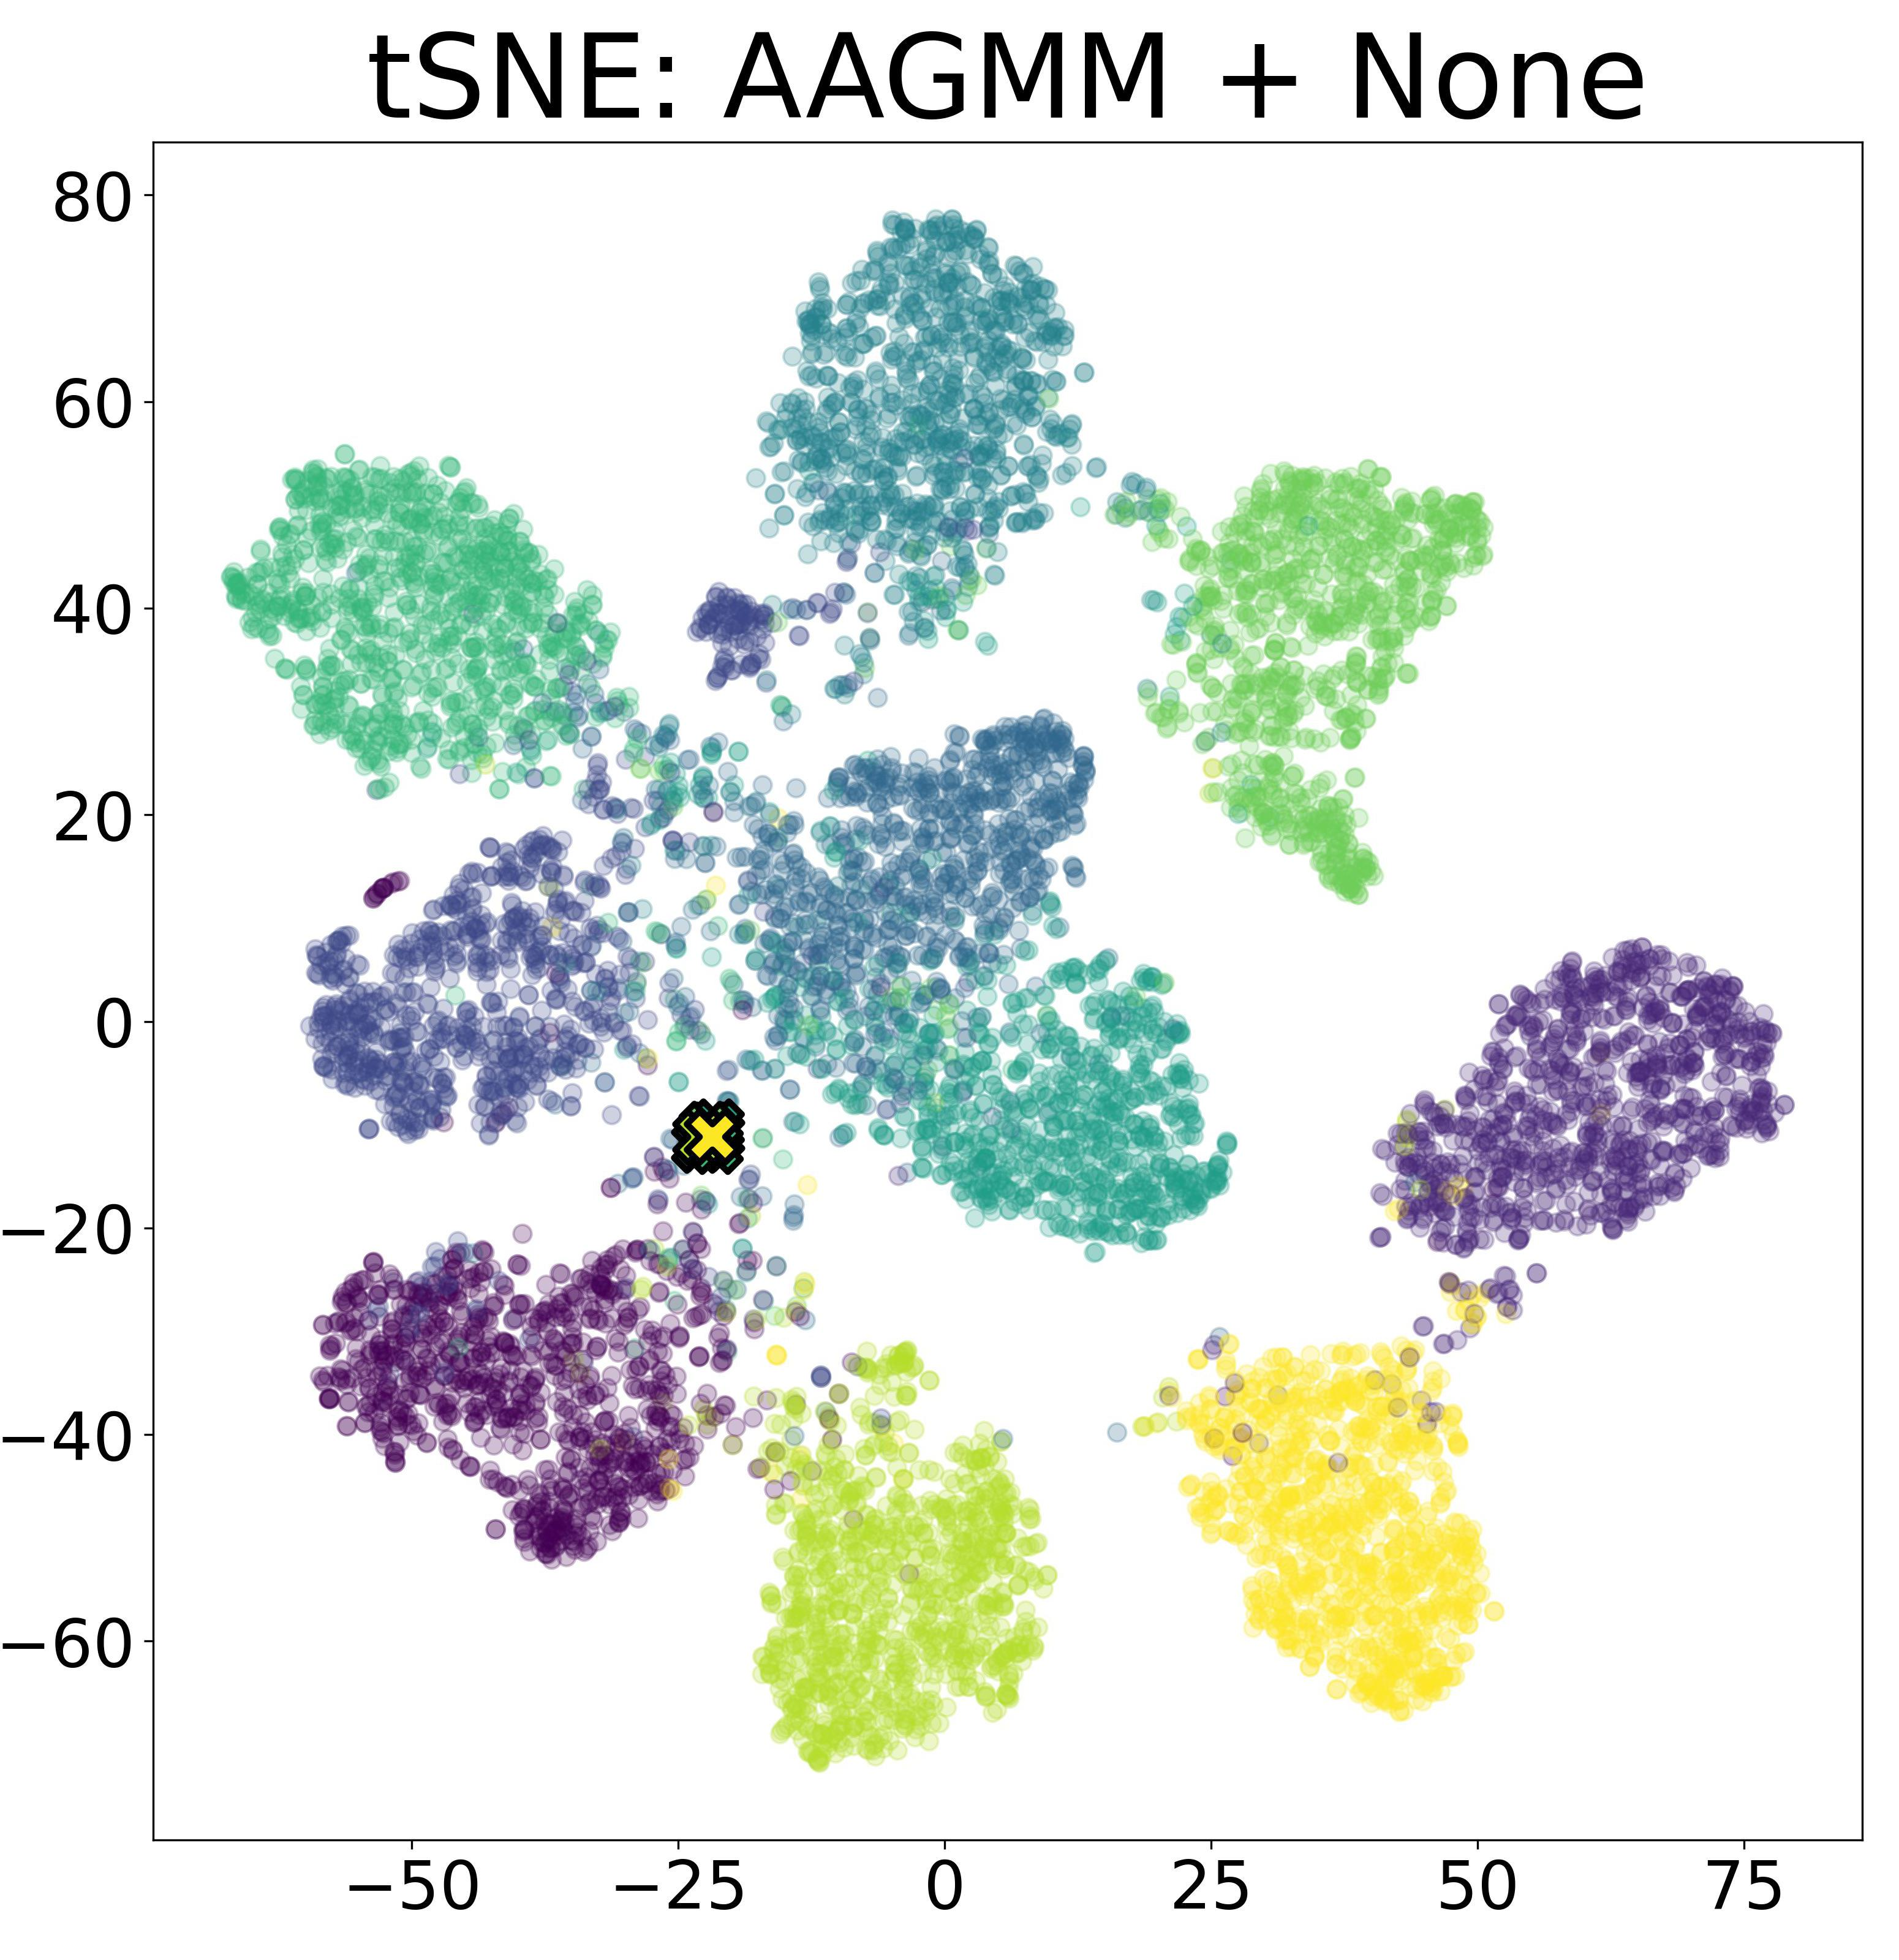
\includegraphics[width=.5\columnwidth]{figures/id-00000132-tsne.jpg}}
	%	\subfloat{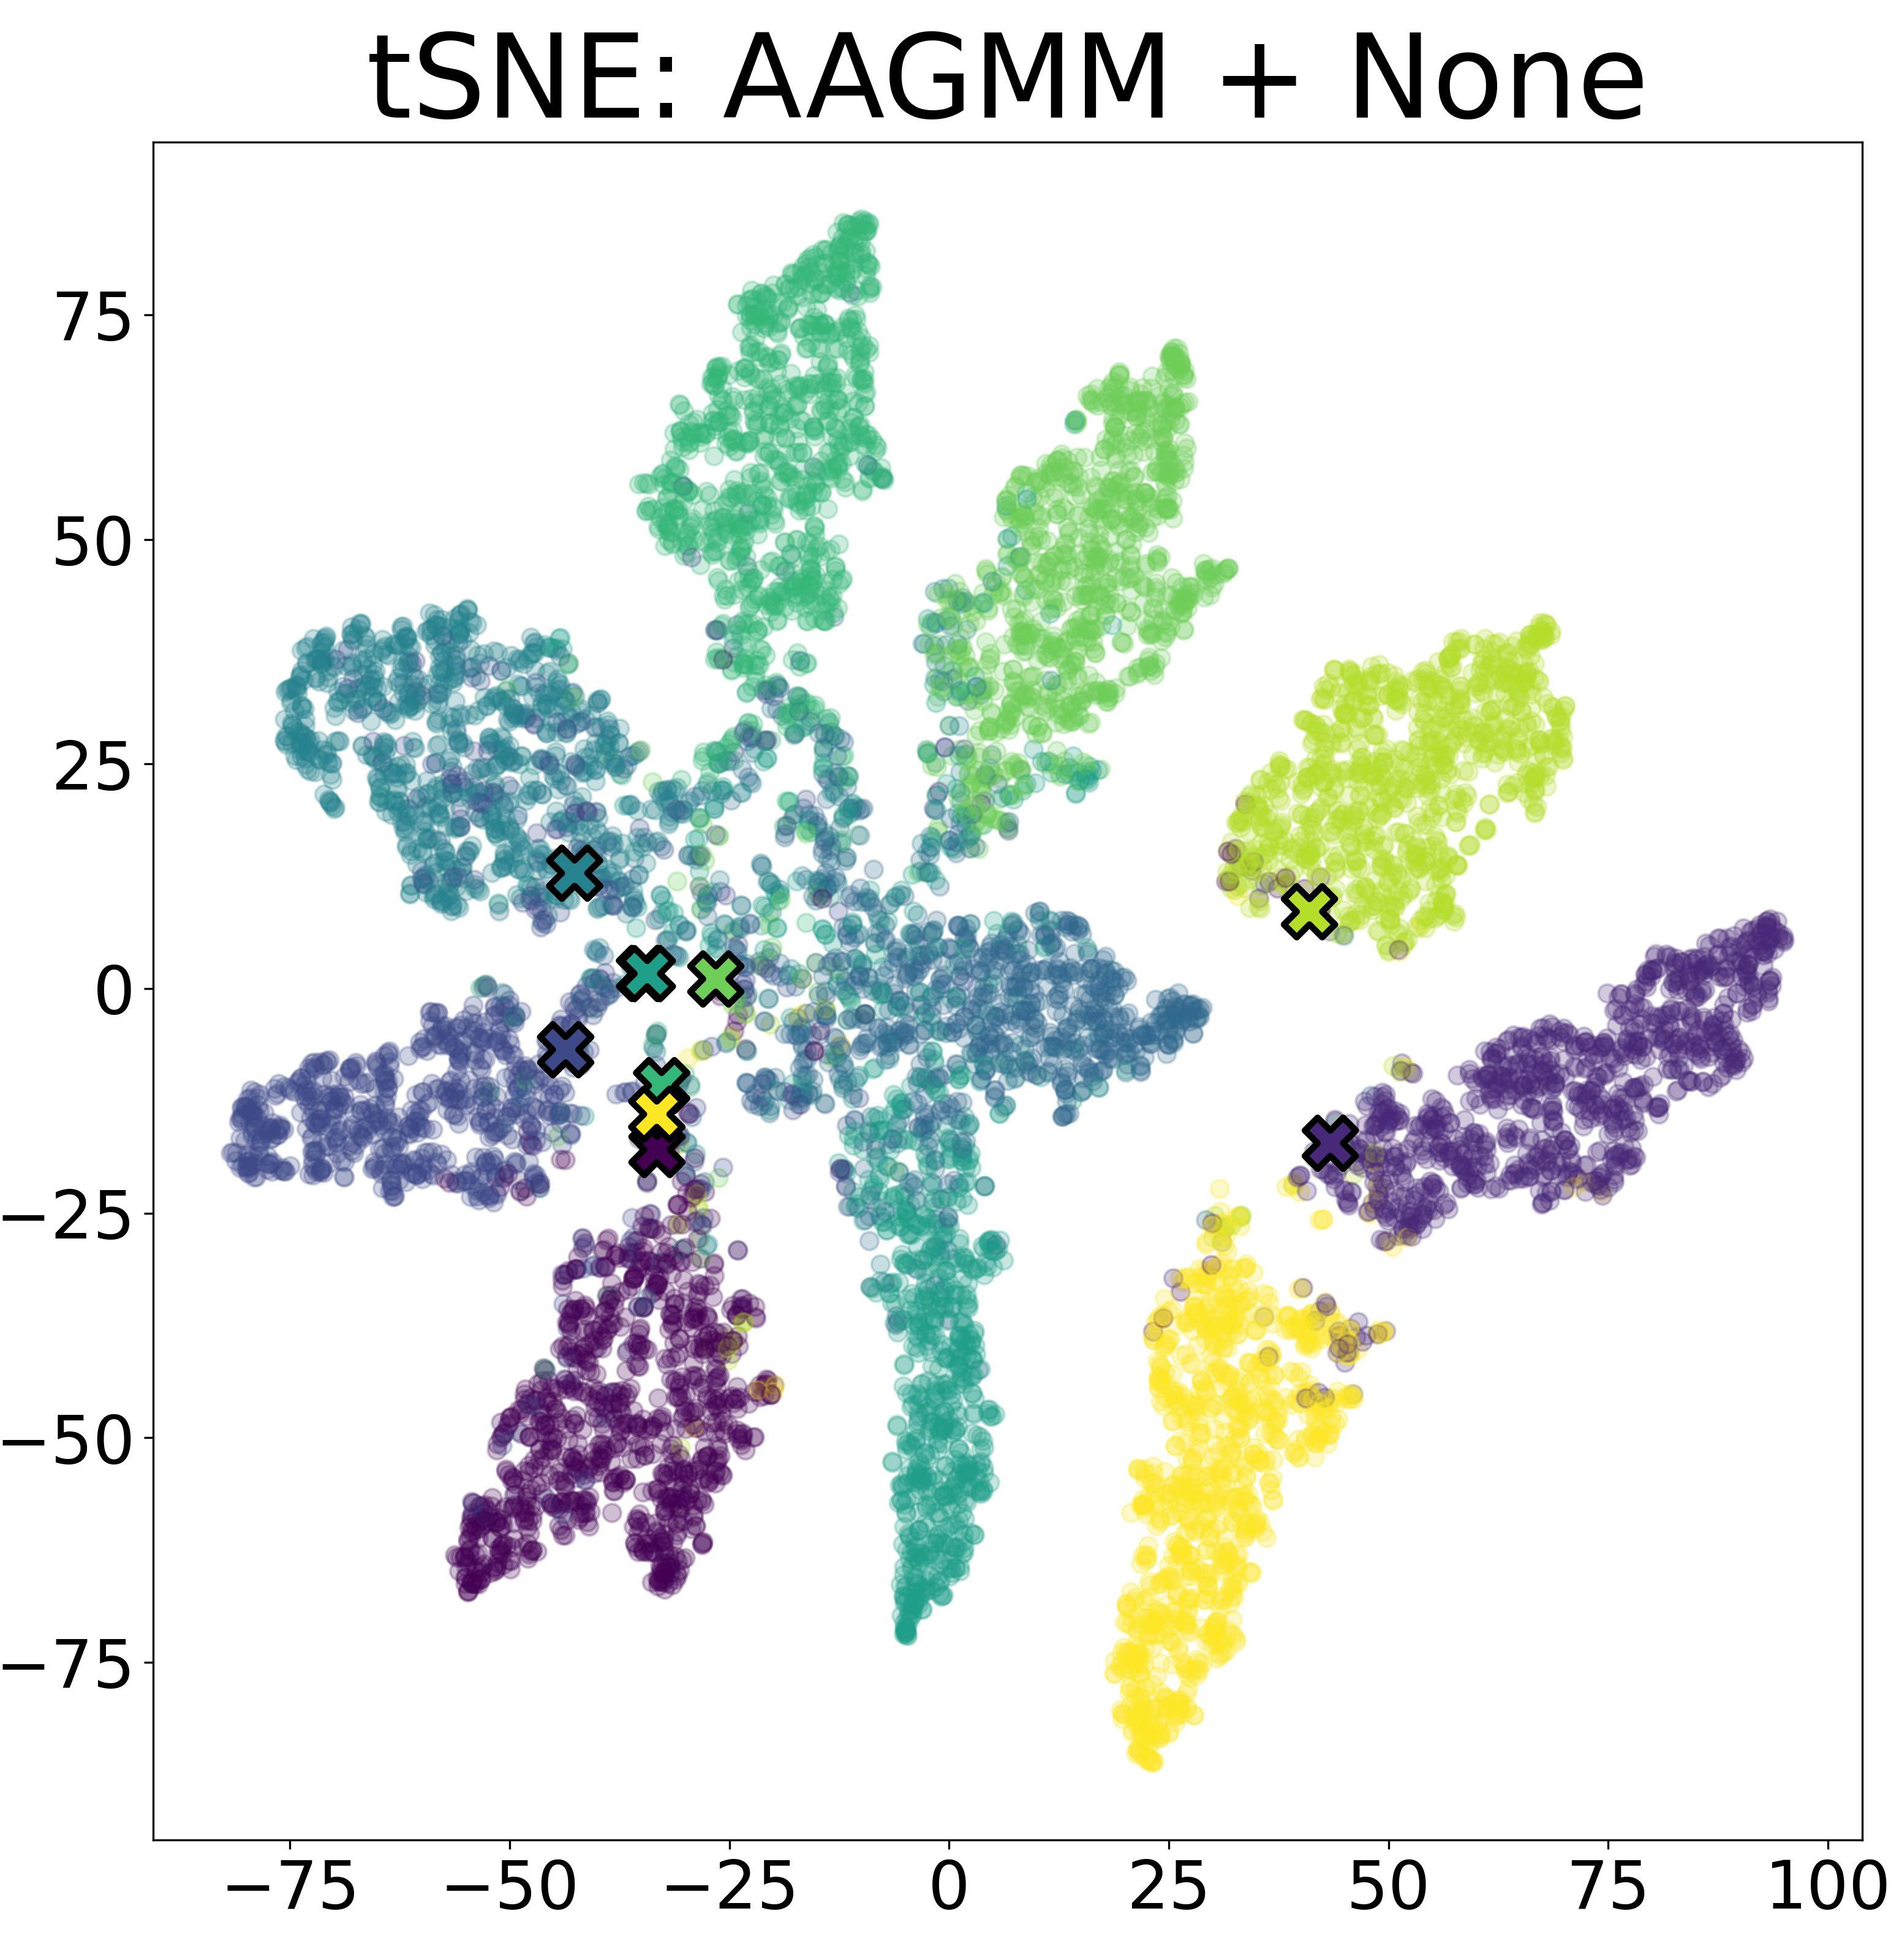
\includegraphics[width=.5\columnwidth]{figures/id-00000020-tsne.jpg}}
	%	\\
	%	\subfloat{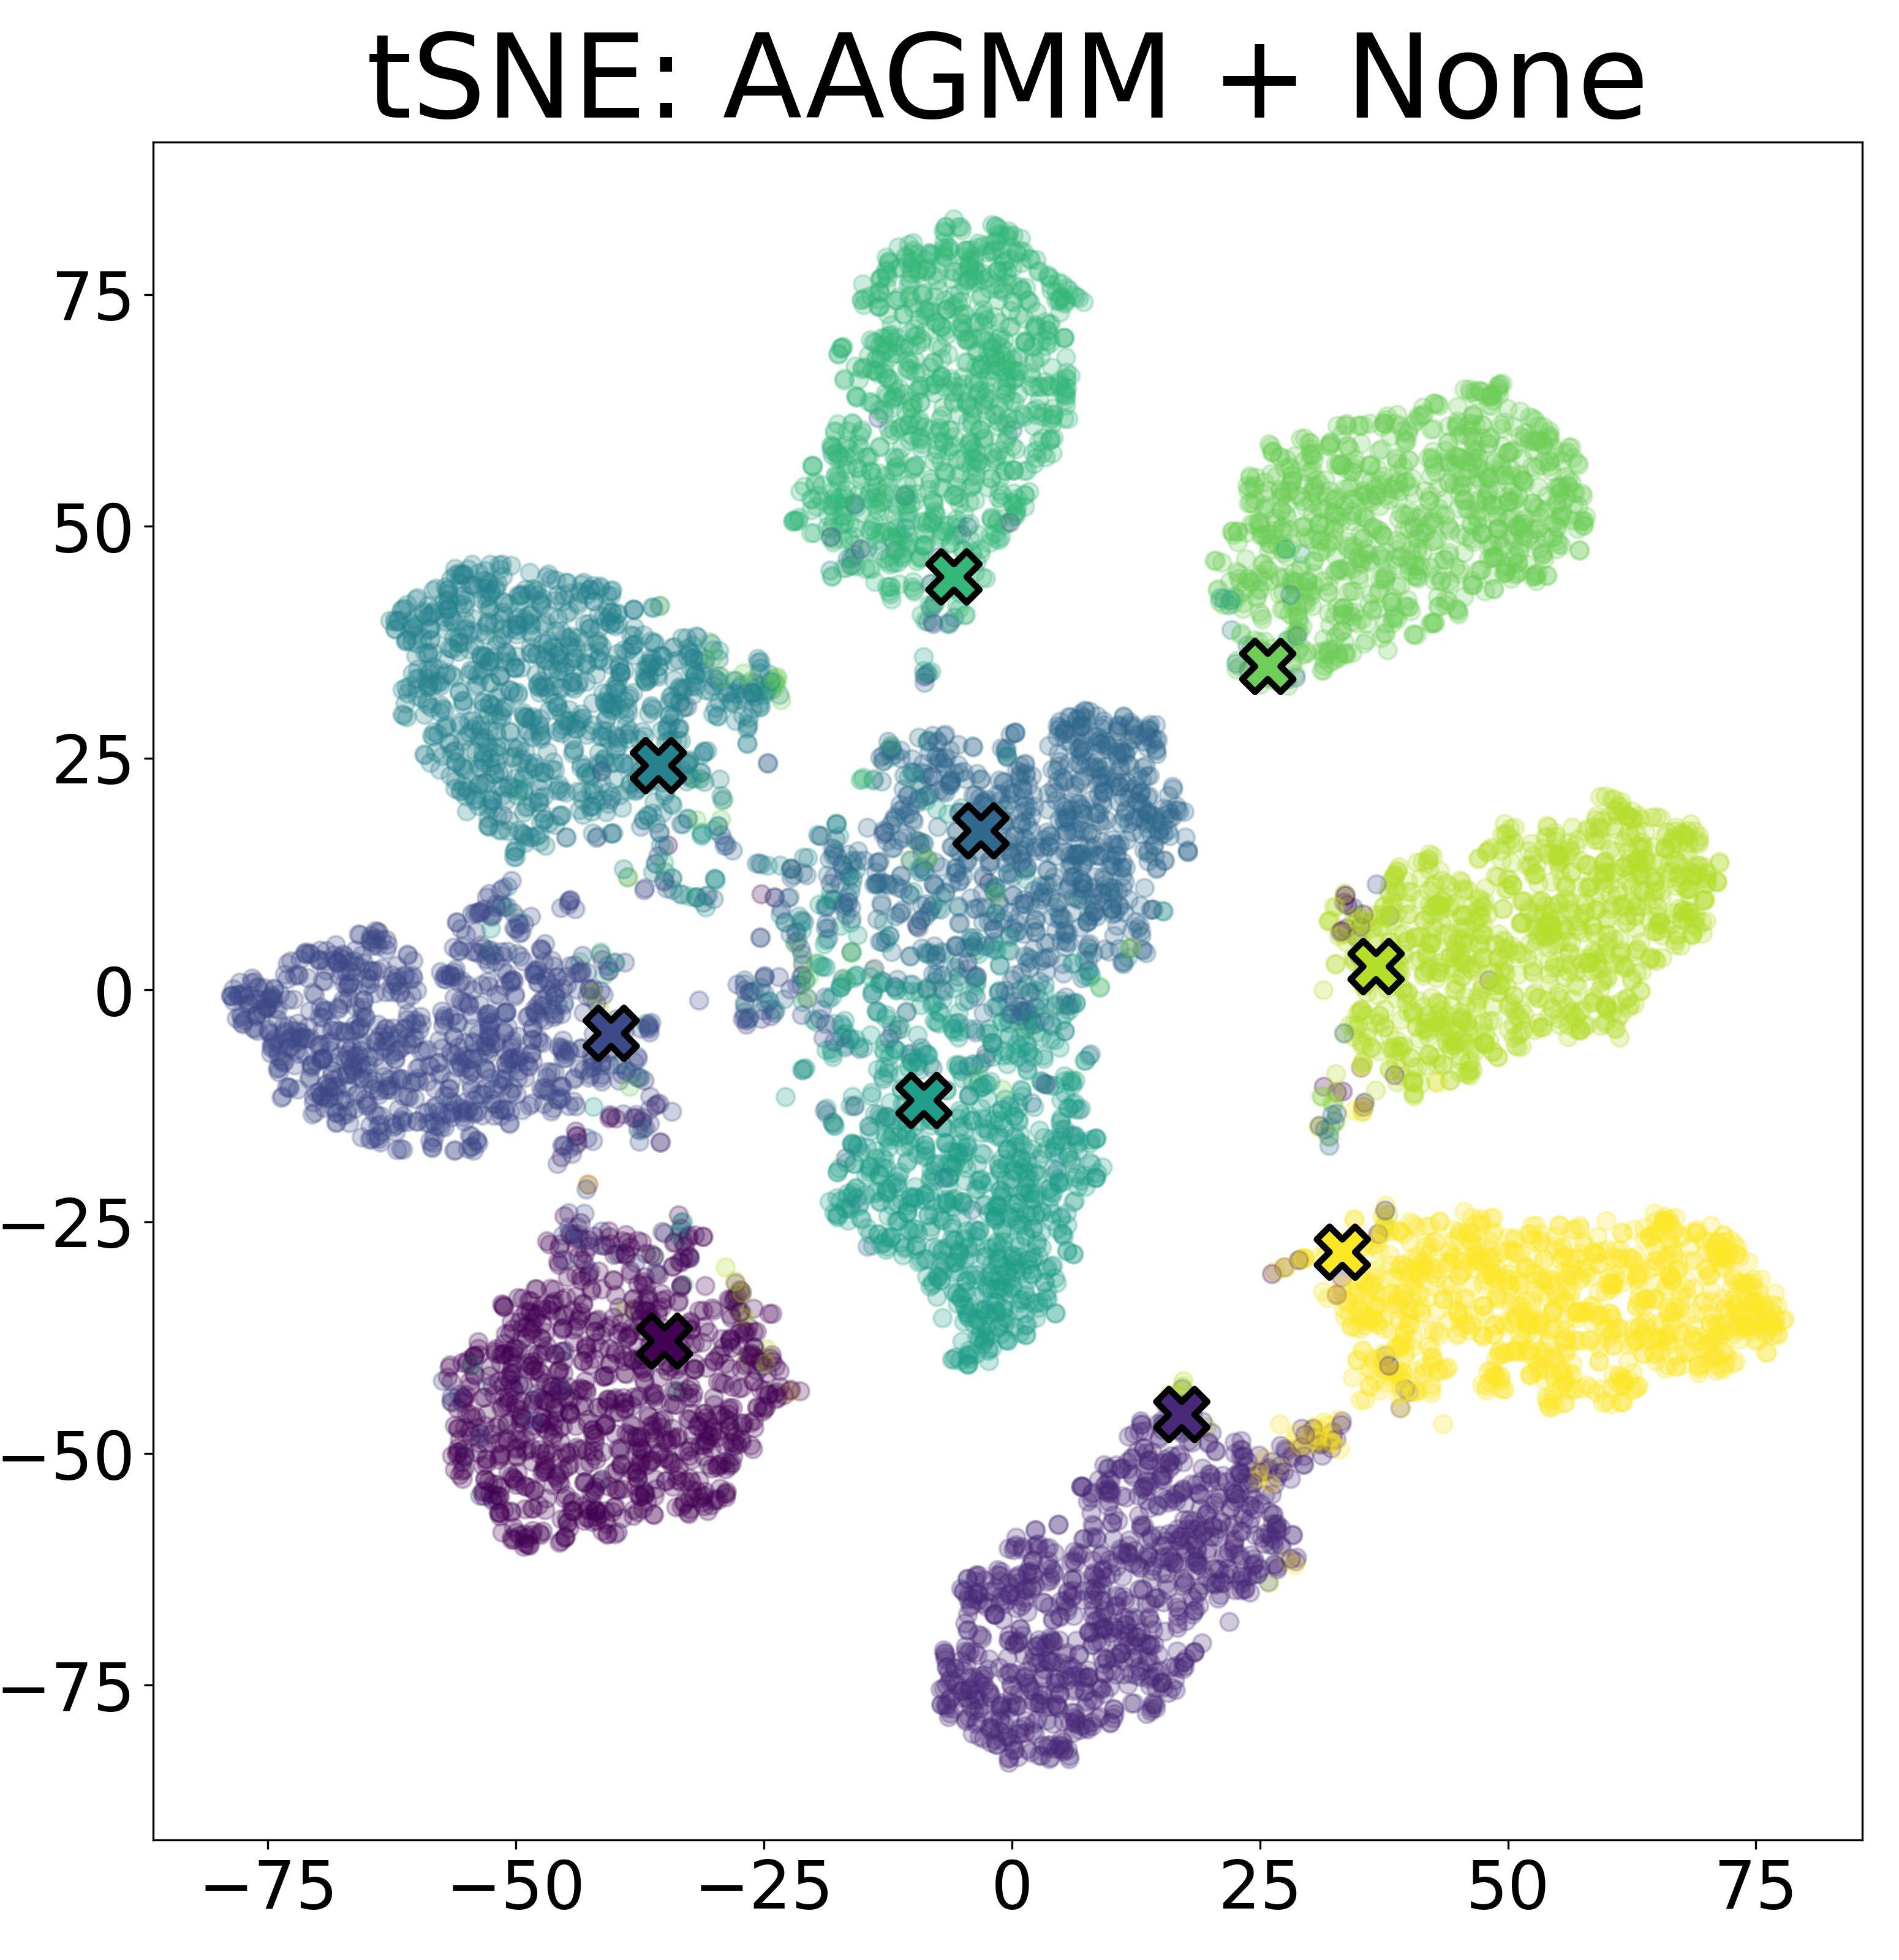
\includegraphics[width=.5\columnwidth]{figures/id-00000120-tsne.jpg}}
	%	\subfloat{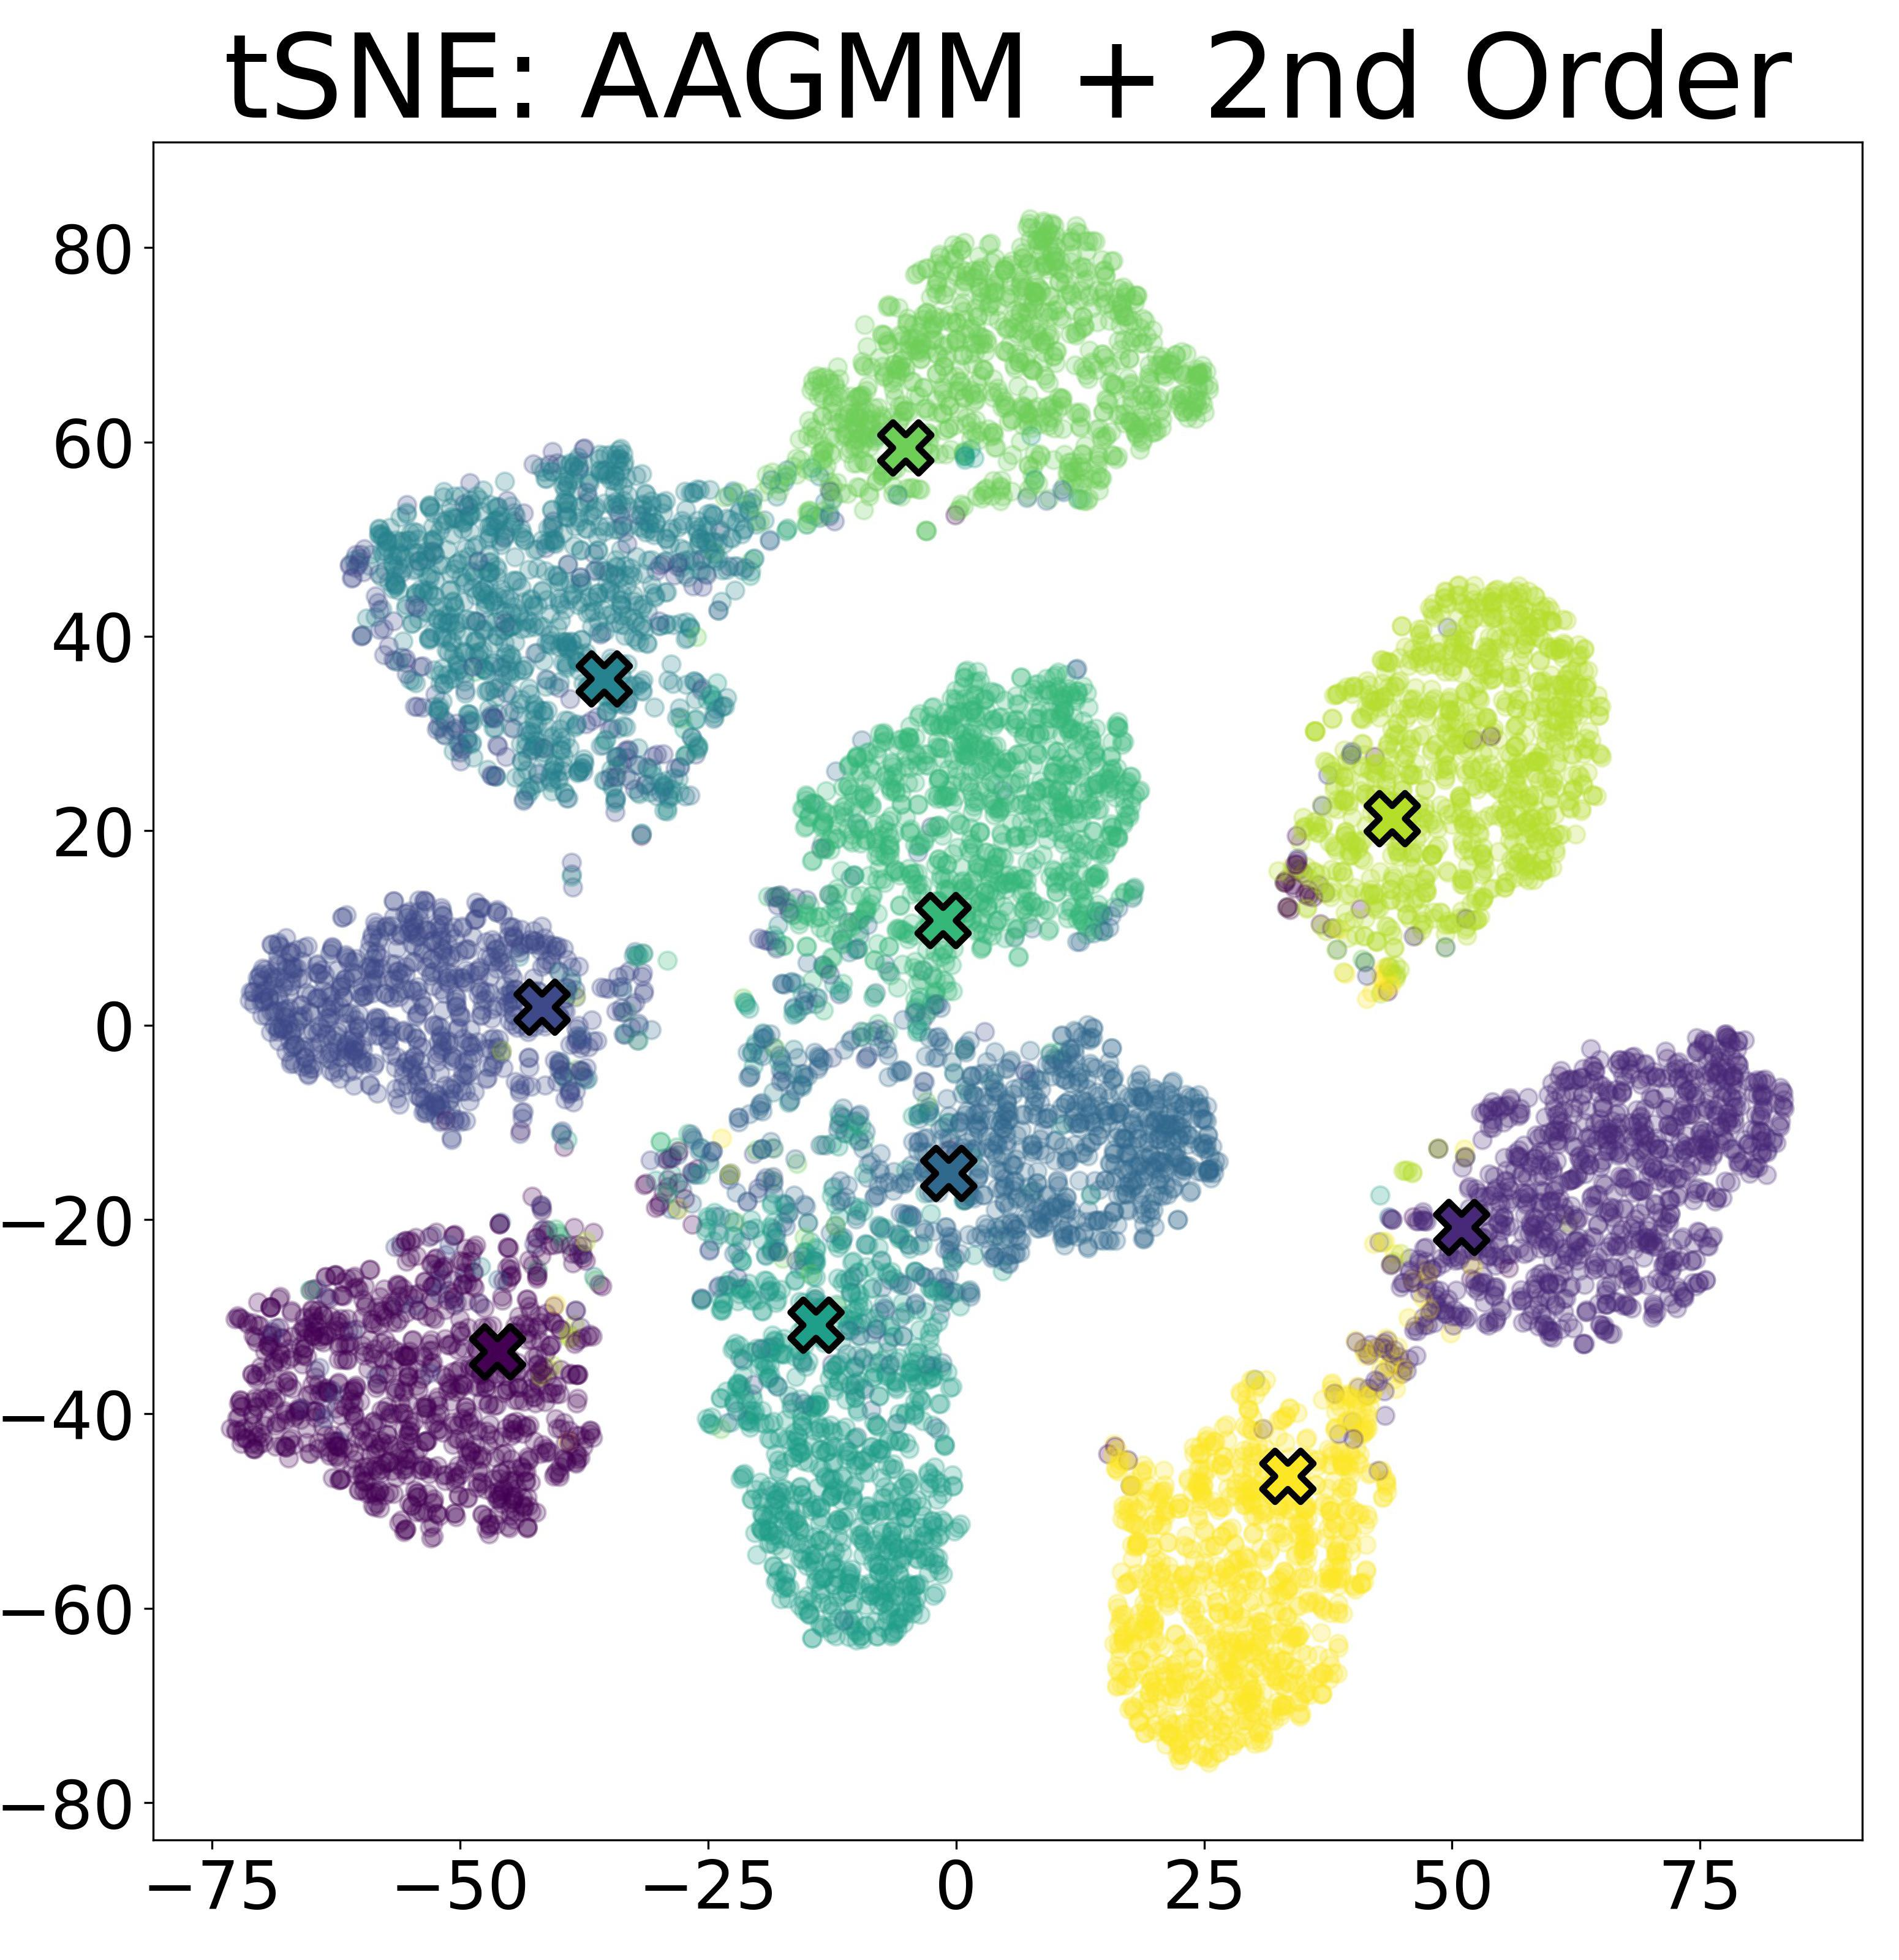
\includegraphics[width=.5\columnwidth]{figures/id-00000054-tsne.jpg}}
	\begin{subfigure}[t]{.49\columnwidth}
		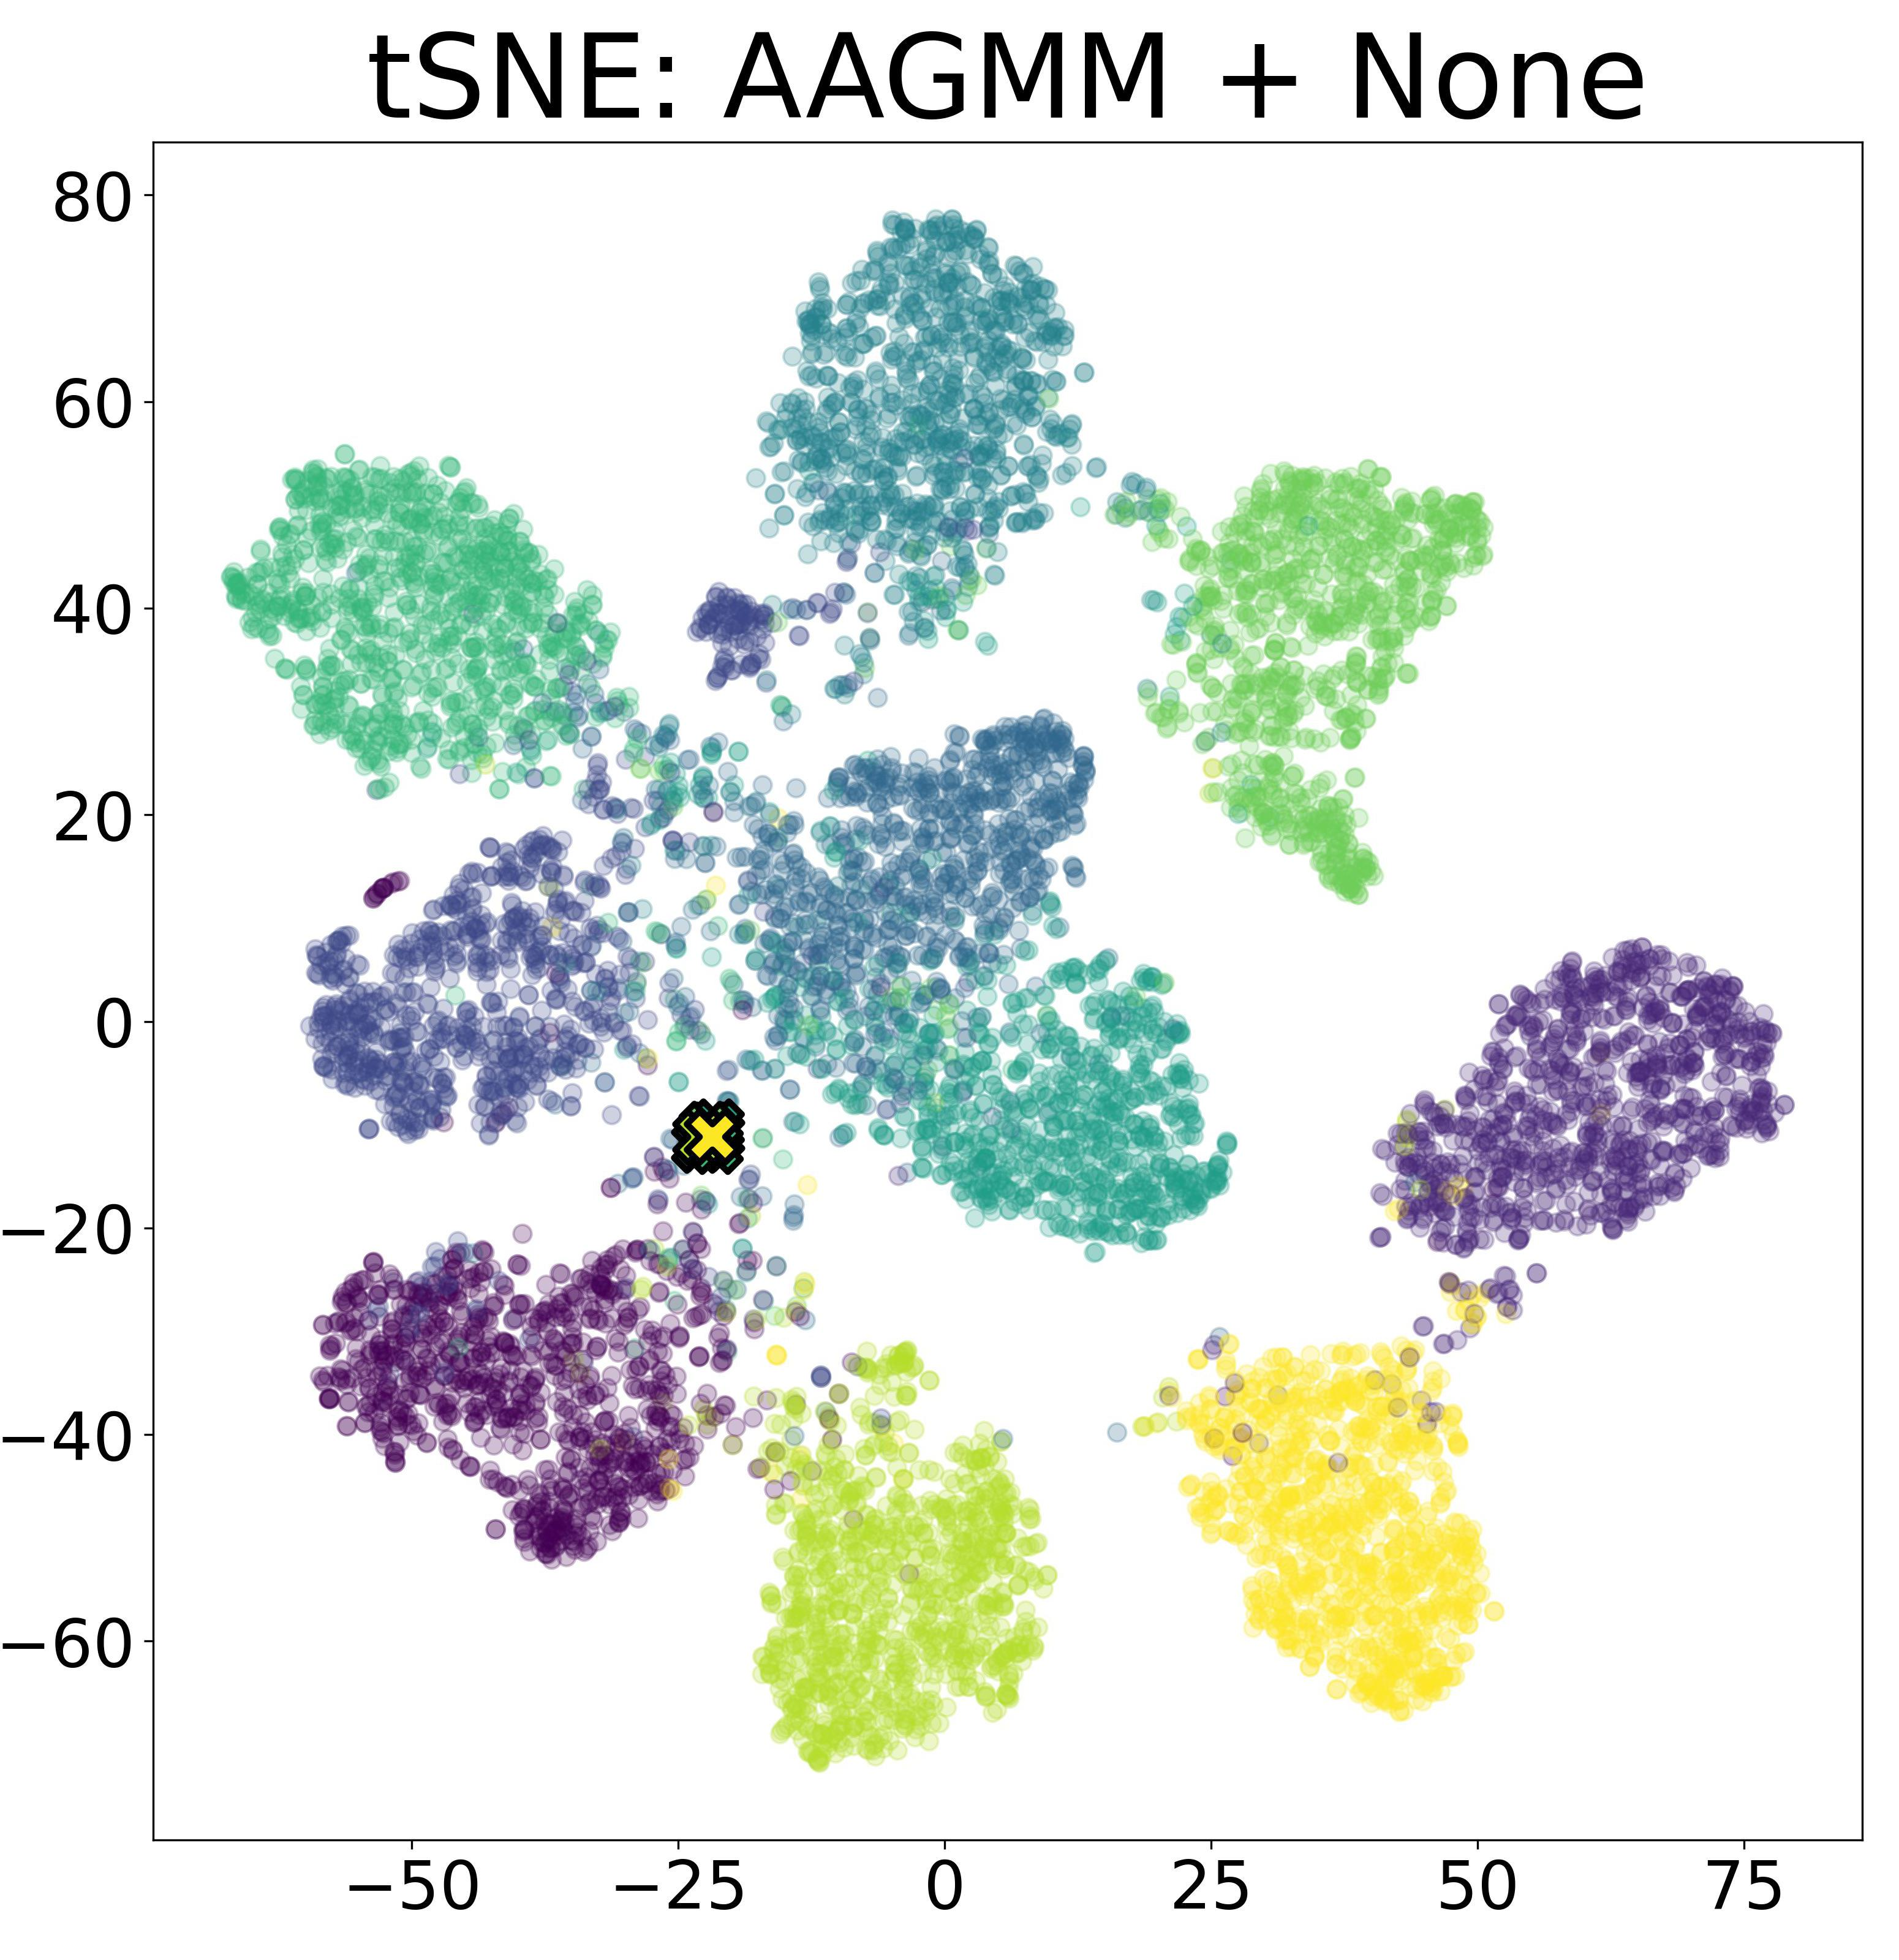
\includegraphics[width=\textwidth]{figures/id-00000132-tsne.jpg}
		\subcaption{}
	\end{subfigure}
	\begin{subfigure}[t]{.49\columnwidth}
		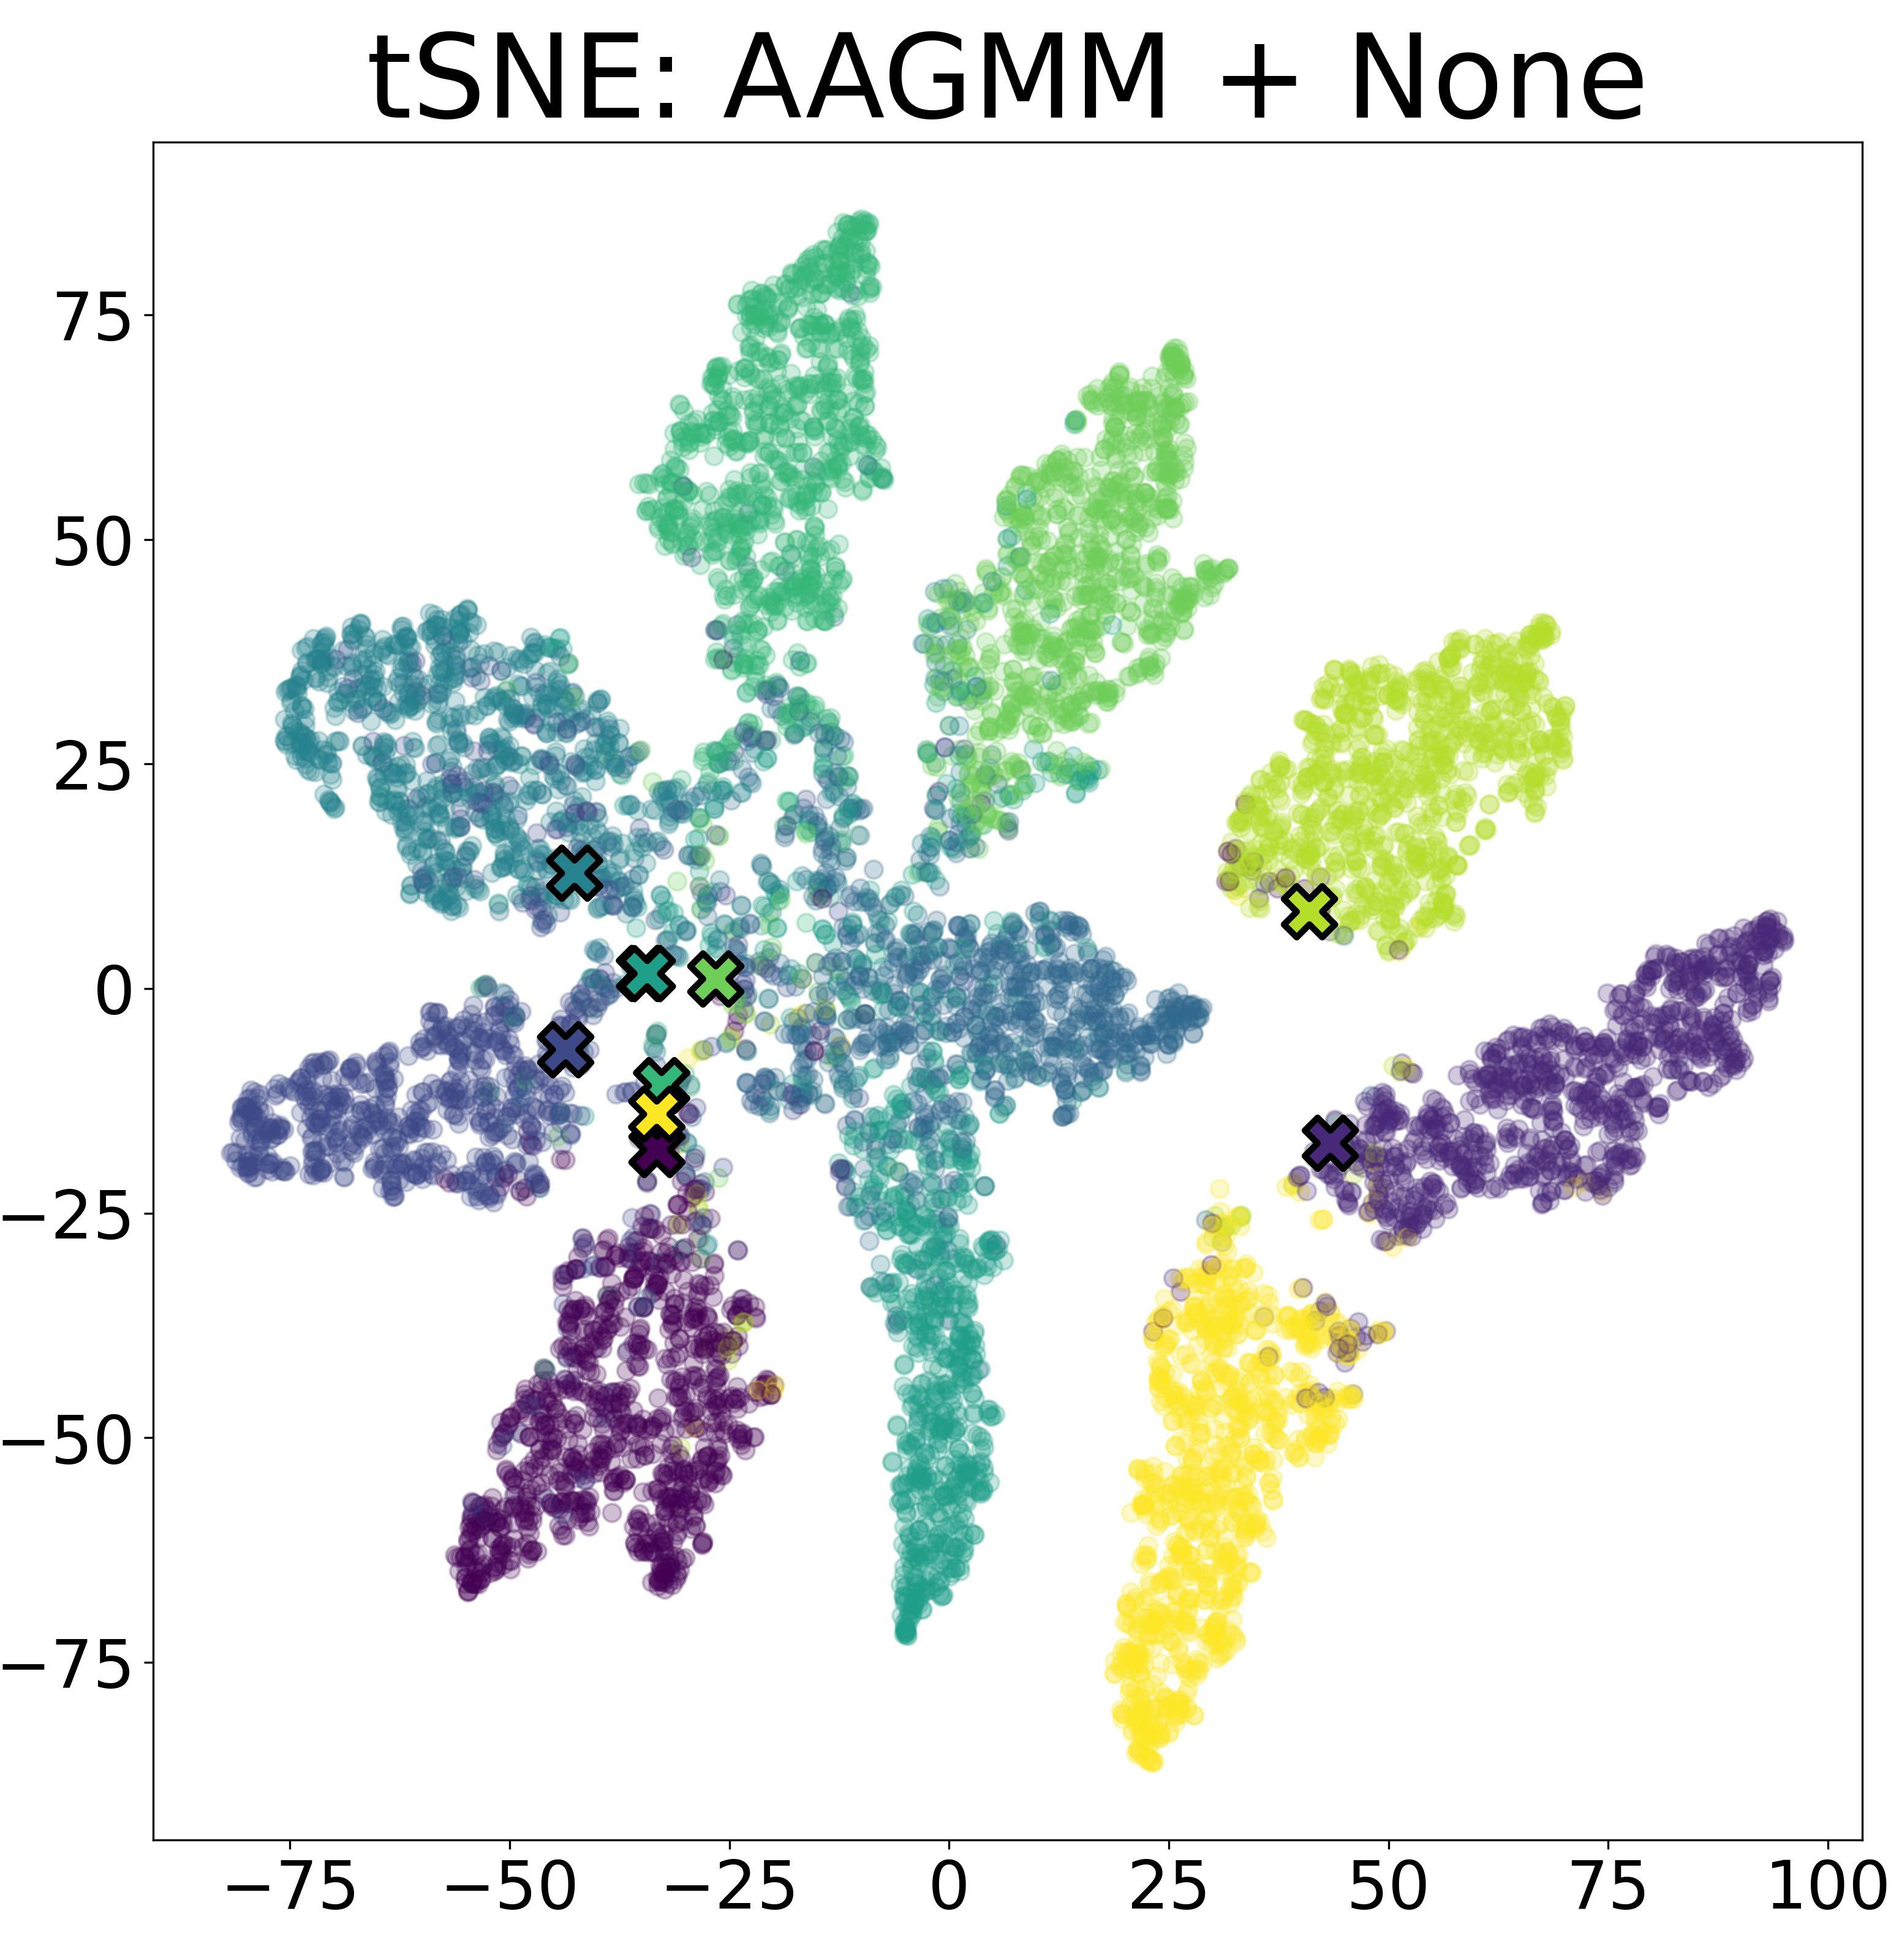
\includegraphics[width=\textwidth]{figures/id-00000020-tsne.jpg}
		\subcaption{}
	\end{subfigure}
	\begin{subfigure}[t]{.49\columnwidth}
		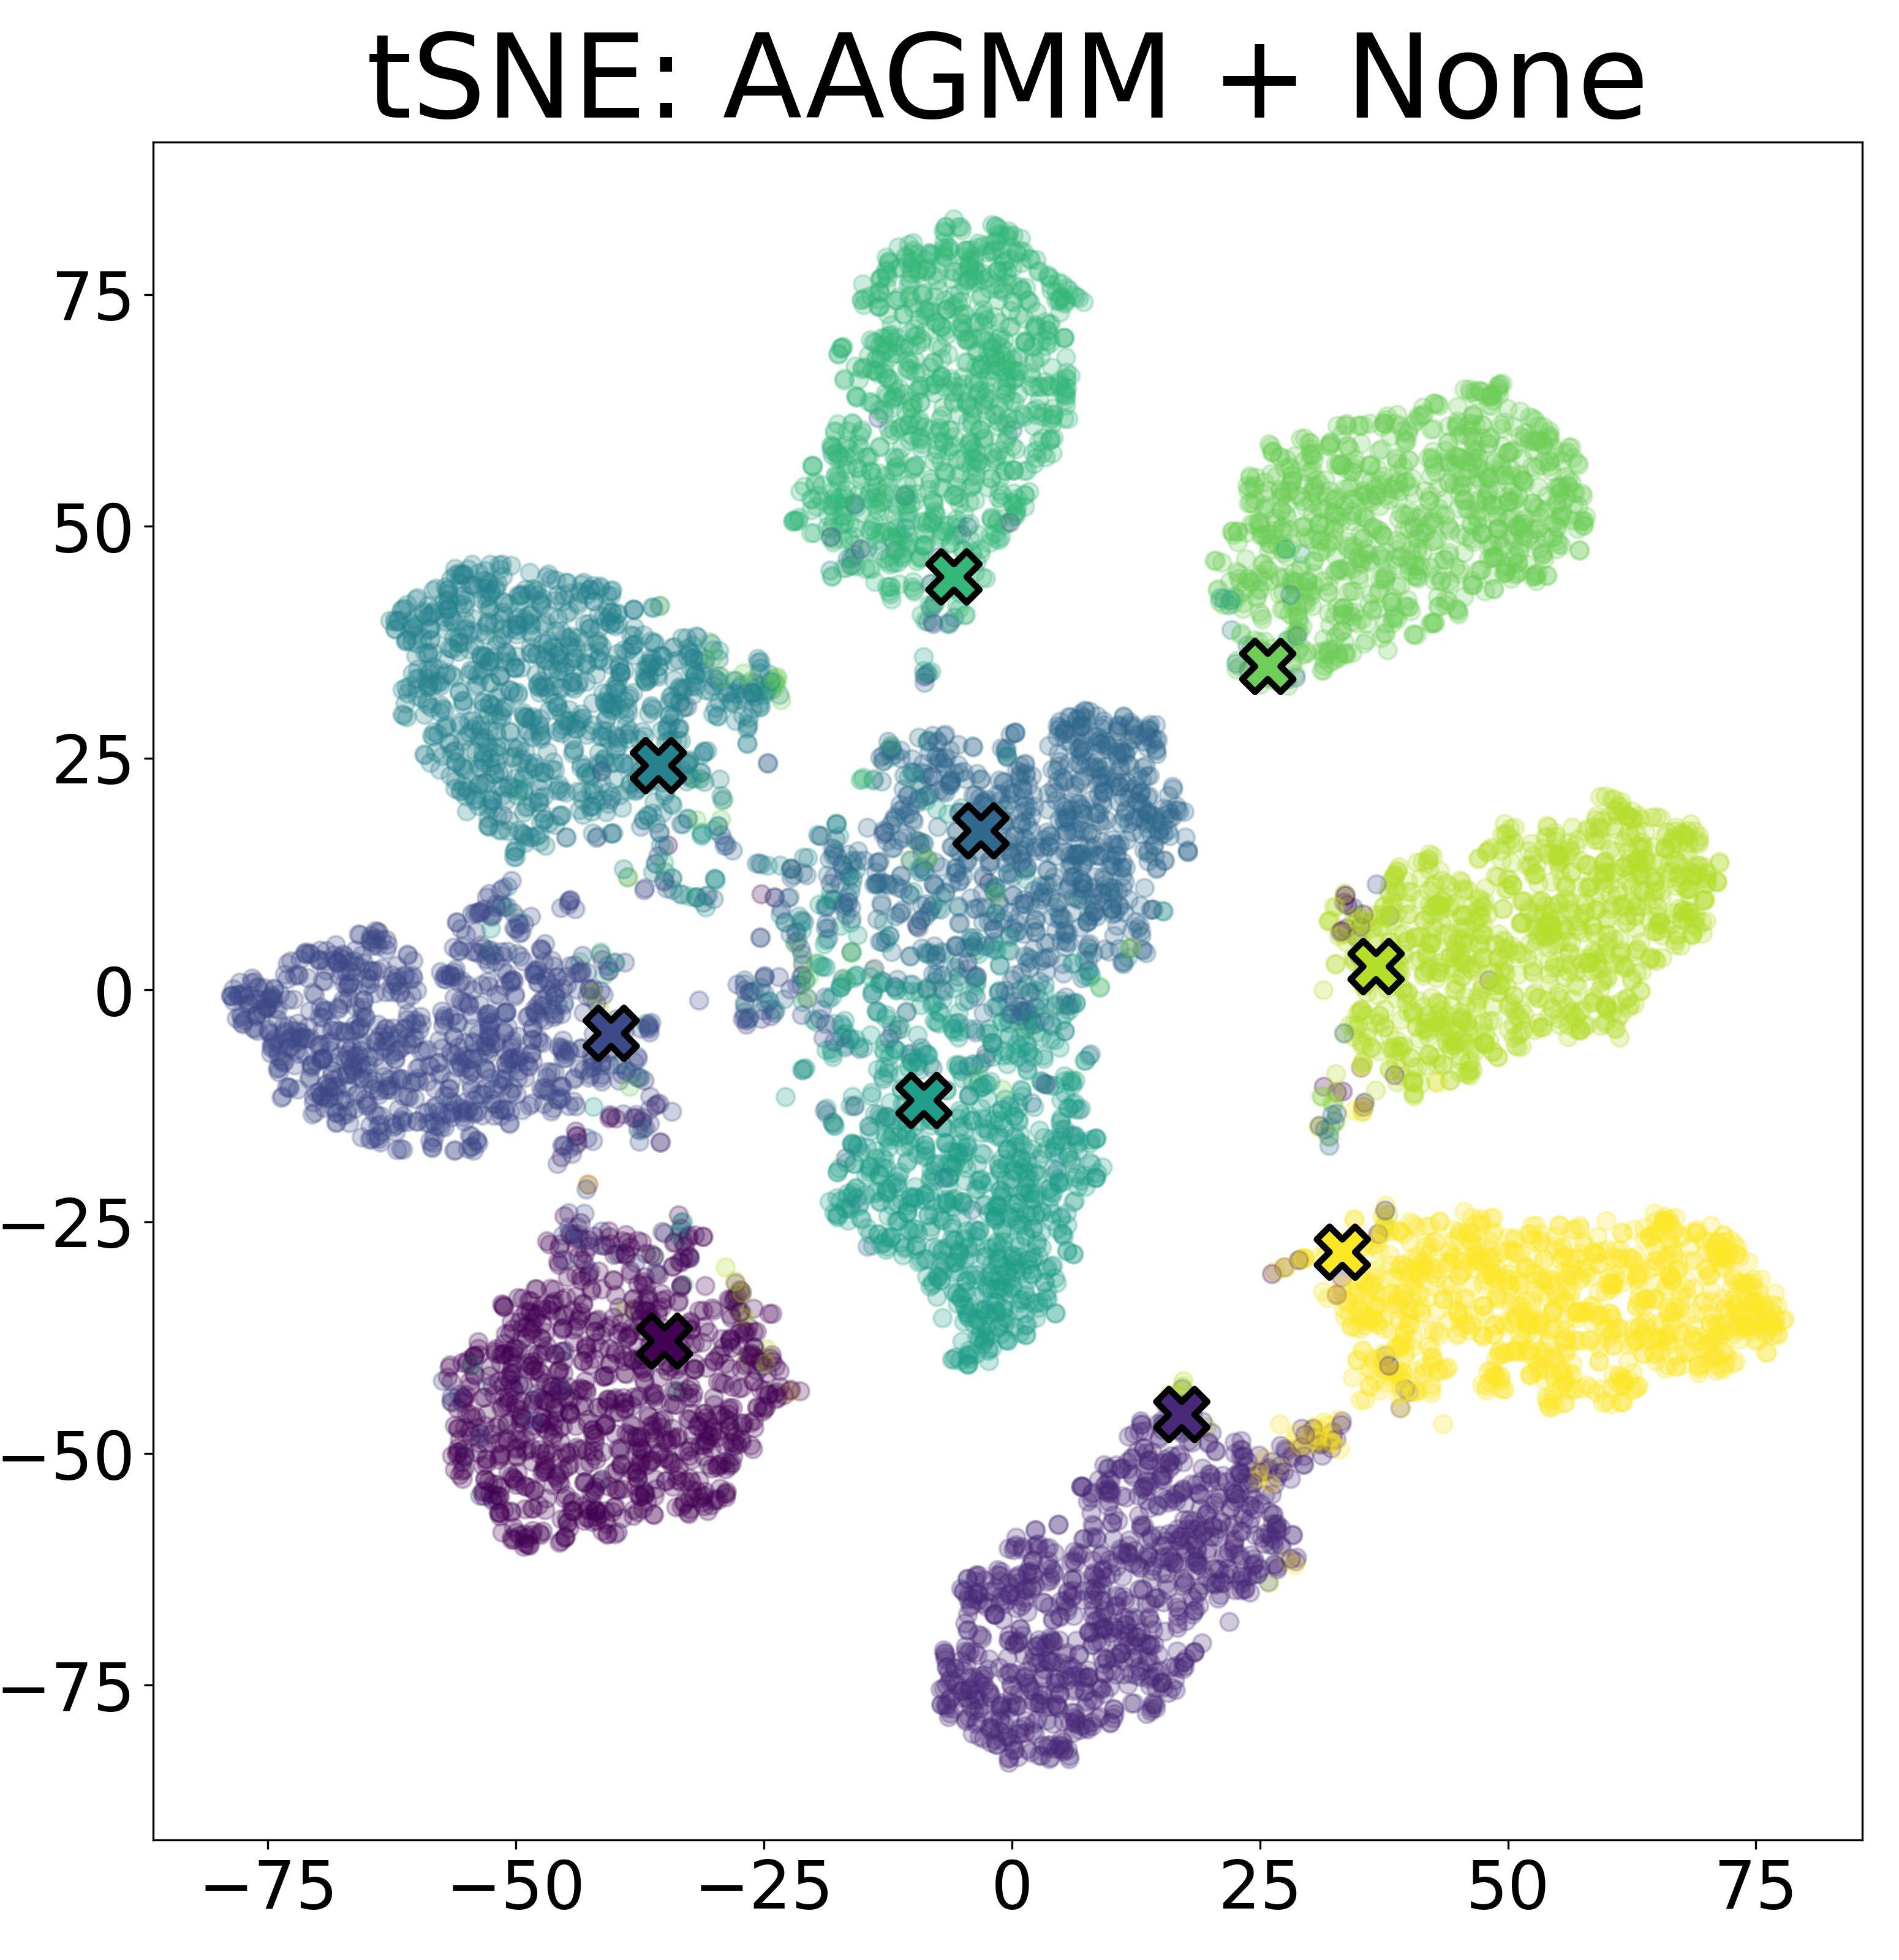
\includegraphics[width=\textwidth]{figures/id-00000120-tsne.jpg}
		\subcaption{}
	\end{subfigure}
	\begin{subfigure}[t]{.49\columnwidth}
		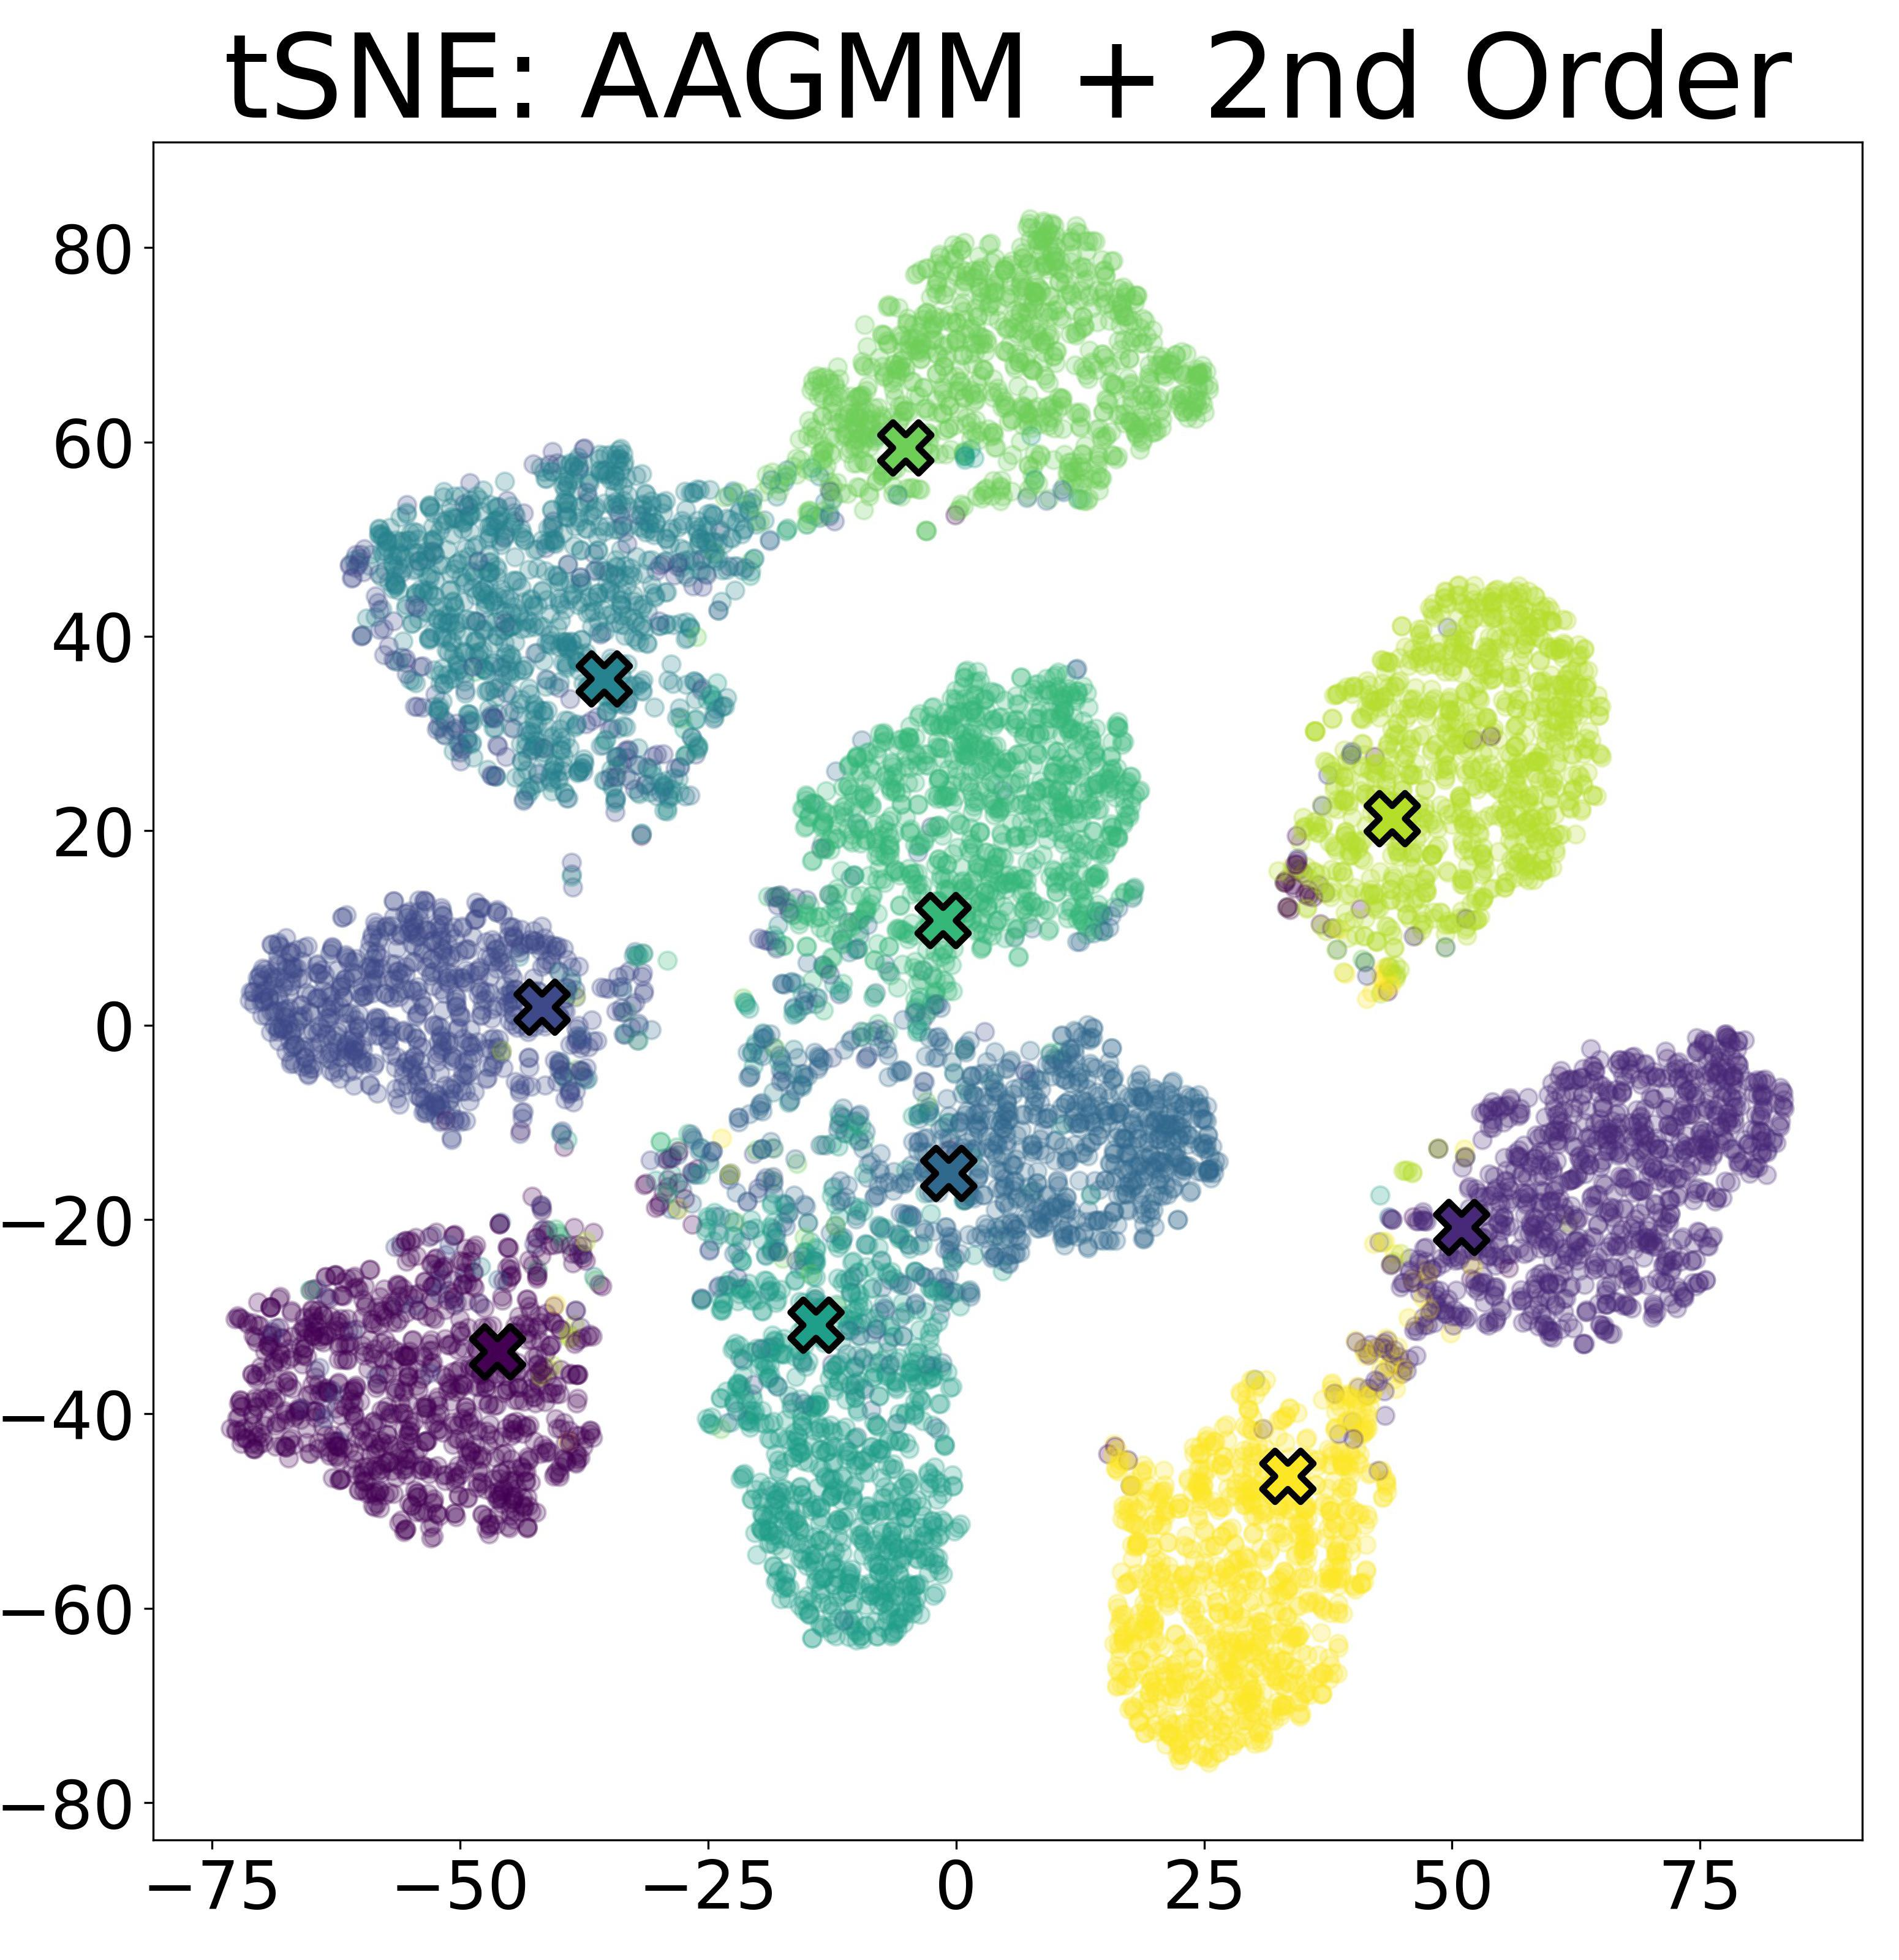
\includegraphics[width=\textwidth]{figures/id-00000054-tsne.jpg}
		\subcaption{}
	\end{subfigure}
	
	%	\includegraphics[width=0.9\linewidth]{example-image-a}
	\caption{t-SNE plot of fully trained and reasonably accuracy AAGMM model's latent embedding space (with the learned cluster centers marked with X's). Depending on the run, the AAGMM cluster centers will be degenerate (top left), non-degenerate but still mis-aligned with the clusters (top right), acceptably aligned (bottom left), or well aligned with the underlying clusters when a 2nd order constraint is employed (bottom right).} 
	\label{fig:cifar10tsneaagmmnone}
\end{figure}


Table \ref{sslcifar10} puts these results in context with the current SSL SOTA for CIFAR-10 at 40 labels and demonstrates that this methodology still requires improvement before it is competitive with the latest methods. 

\begin{table}[htbp]
	\begin{tabular}{c|cc}
		Method          & \multicolumn{2}{c}{CIFAR-10} \\ \hline
		Label Count     & 40            & 250           \\
		%Supervised & $77.18$ \scriptsize{$\pm1.32$}   & $56.24$ \scriptsize{$\pm3.41$}   \\ 
		\hline
		FixMatch\cite{sohn2020fixmatch}   & $13.81$ \scriptsize{$\pm3.37$}   & $5.07$ \scriptsize{$\pm0.65$}     \\
		FlexMatch\cite{zhang2021flexmatch}  & $4.97$ \scriptsize{$\pm0.06$}    & $4.98$ \scriptsize{$\pm0.09$}    \\
		FreeMatch\cite{wang2022freematch}  & $4.90$ \scriptsize{$\pm0.29$}    & $4.98$ \scriptsize{$\pm0.09$}    \\
		SimMatchV2\cite{zheng2023simmatchv2} & $4.90$ \scriptsize{$\pm0.04$}    & $5.04$ \scriptsize{$\pm0.09$}    \\ \hline
		Ours (AAGMM+None)    & $8.77$ \scriptsize{$\pm 2.89$}           & $5.91$ \scriptsize{$\pm 0.34$}  \\
		Ours (KMeans+2ndOrder)    & $10.11$ \scriptsize{$\pm 2.79$}           & $6.84$ \scriptsize{$\pm 1.25$}  
		
	\end{tabular}
	\caption{Error rate \% for CIFAR-10 SSL benchmark comparing to state of the art results. Results for previously published methods are drawn from USB \cite{wang2022usb} except for FreeMatch\cite{wang2022freematch} and SimMatchV2\cite{zheng2023simmatchv2} publications.}
	\label{sslcifar10}
\end{table}



\section{Discussion}

The proposed MoM embedding constraint has at least one significant downside, it requires exponentially increasing amounts of GPU memory for each successive moment penalty included.
This limits the current practicality of these MoM constraints. 
Additional optimization and/or avoiding the explicit creation of both the $nth$ order moment and its target value on device would likely improve the usability.

Semi-supervised learning is highly sensitive to both which samples are selected for the labeled population \cite{sohn2020fixmatch} and the stochasticity of the training process itself.
Given identical starting random seeds, and identical labeled samples, training stochasticity will quickly cause models to diverge, resulting in vastly different final results.
Anecdotally its appears worse in semi-supervised methods than fully supervised models.
To characterize this variance, and hence how much one can trust the error bars for Table \ref{table1} and \ref{tablemaxcf10}, we took a few final layer configurations and ran them $N=5$ times with the same seed.
Table \ref{tab:runseedvariability} showcases the run-to-run variances for models that started out identical.
Interestingly enough, the AAGMM models converge with much lower variance than the KMeans models.
This contrasts with the KMeans layer being significantly simpler than AAGMM, both mathematically and implementation-wise.

\begin{table}[h!]
	\begin{tabular}{r|c|c|c|c}
		\multicolumn{5}{c}{Identical Seed Runs on CIFAR-10 at 40 Labels}\\
		\hline
		& \small{\makecell{AAGMM\\+2nd Order}} & \small{\makecell{KMeans\\+2nd Order}} & \small{\makecell{AAGMM\\+None}} & \small{\makecell{KMeans\\+None}} \\
		\hline
		Run 1 & $87.5$ & $86.9$ & $71.2$ & $86.5$ \\
		Run 2 & $85.6$ & $91.2$ & $67.9$ & $85.4$ \\
		Run 3 & $84.8$ & $77.7$ & $75.8$ & $86.0$ \\
		Run 4 & $85.3$ & $87.6$ & $69.5$ & $87.6$ \\
		Run 5 & $85.2$ & $83.7$ & $78.9$ & $85.7$ \\
	\end{tabular}
	\caption{Test accuracy for independent training runs with the same random seed for various final layer configurations. All runs use the 128D (baseline) model latent embedding dimensionality. All runs use the same labeled samples.}
	\label{tab:runseedvariability}
\end{table}

Future work in this area should explore both accuracy improvements as well as implementation optimization to ensure the proposed novel final layers are not prohibitively memory expensive.
Additionally, one should explore how to best take advantage of the better behaved latent embedding space to improve data efficiency for model training. 

We demonstrate a novel fully differentiable Axis-Aligned Gaussian Mixture Model with Method of Moments based latent embedding space constraints to improve the generative inlier/outlier performance of image classification deep learning models. 
This preliminary work constructs those novel layers with the associated constraints, and demonstrates reasonable performance on challenging benchmark semi-supervised learning tasks.



{
	\small
	\bibliographystyle{ieeenat_fullname}
	\bibliography{refs}
}


\end{document}